%For two sided printing
% \documentclass[a4paper,12pt,twoside,onecolumn,openright,final]{memoir} %for printing two sided

%For one sided printing
\documentclass[a4paper,12pt,oneside,onecolumn,final]{memoir} %for electronic viewing and one-sided printing

%Memoir class geometry, stole it from online manual
\settrimmedsize{297mm}{210mm}{*}
\setlength{\trimtop}{0pt}
\setlength{\trimedge}{\stockwidth}
\addtolength{\trimedge}{-\paperwidth}
\settypeblocksize{634pt}{448.13pt}{*} %original is 634
\setulmargins{4cm}{*}{*} %original is 4 lol
\setlrmargins{*}{*}{1.5}
\setmarginnotes{17pt}{51pt}{\onelineskip}
\setheadfoot{\onelineskip}{2\onelineskip}
\setheaderspaces{*}{2\onelineskip}{*}
\checkandfixthelayout

\usepackage[nodate, 12hr]{datetime} %for time and date
\title{Brief Notes on Differential Geometry}
\author{Lim Kian Hwee}
\date{\small Last updated: \today, \currenttime} %leave blank if dont want date

%Packages for paper formatting, figures, hyperref, etc
\usepackage{microtype}
\usepackage{xcolor}
\usepackage{parskip} %package to tweak paragraph skipping
\usepackage{graphicx}
\usepackage[space]{grffile} %For file names with spaces
\graphicspath{{./Figures/}}
\usepackage{chngcntr}
\counterwithin{figure}{chapter}
\counterwithin{footnote}{chapter}
\usepackage{float}
\usepackage{comment} 
\usepackage{wrapfig}
\setcounter{tocdepth}{1} %stops TOC numbering at sections
\setsecnumdepth{subsection} %numbers subsections
\PassOptionsToPackage{hyphens}{url}
\usepackage[hidelinks]{hyperref}
\hypersetup{
    colorlinks,
    linkcolor={blue!50!black},
    citecolor={blue!50!black},
    urlcolor={blue!80!black}
}
%For quotation marks to behave well
\usepackage{csquotes}
% \MakeOuterQuote{"}

%Blind text
\usepackage[english]{babel}
\usepackage{blindtext}
\blindmathtrue

%Math packages
\usepackage{amsmath}
\usepackage{amssymb}
\usepackage{mathtools}
\numberwithin{equation}{chapter} %numbers equations according to chapters
%\allowdisplaybreaks %equations in environment can page break
\usepackage{physics}
\usepackage{amsthm}
\theoremstyle{plain}
\newtheorem{theorem}{Theorem}[chapter]
\theoremstyle{remark}
\newtheorem{corollary}{Corollary}[theorem]
\theoremstyle{plain}
\newtheorem{lemma}[theorem]{Lemma}
\theoremstyle{definition}
\newtheorem{definition}{Definition}[chapter]
\theoremstyle{remark}
\newtheorem*{remark}{Remark}
% \usepackage{coloremoji}

%Alternate fonts 
\usepackage{newtxtext,newtxmath} %this is good
% \usepackage{fourier} %this is good
% \usepackage{newpxtext,newpxmath} %this is good

%The rest are...meh
% \usepackage{libertine,libertinust1math} %this is quite good
% \usepackage{fouriernc} %this is quite good
% \usepackage{mathptmx} %looks quite bad

%For new look
% \usepackage{newpxtext} \usepackage[euler-digits]{eulervm} %looks disgusting

\begin{document}
  \frontmatter
  \maketitle
  \begin{KeepFromToc}
    \tableofcontents %optional
  \end{KeepFromToc}
  \chapter{Foreword}
    This set of notes is a summary of the NUS Physics module "Mathematical
    Methods in Physics 3" (or MM3 for short) taken in my fourth year of study
    in NUS. Naturally, the references for this set of notes would be:
    \begin{enumerate}
      \item{PC4274 Lecture Notes and tutorials, Kuldip}
      \item{PC4274 Lecture Notes, Edward Teo (to a small extent)}
    \end{enumerate}
    The purpose of this set of notes is to summarise the key ideas of
    Differential Geometry as I understand it, so that in the future I can
    quickly reference this to get a brief idea of the topic. For more
    detailed treatments, there are textbooks like Frankel, Nakahara, or just
    the lecture notes themselves that are listed above. Unless absolutely
    necessary, no examples will be given.

    Also, Einsten summation convention will be used throughout. I.e, for
    tensors, repeated upper and lower indices are summed over. Sometimes we
    will sum over repeated indices for things that are not tensors, in which case we might sometimes sum over two repeated upper indices, or two repeated lower indices (sloppy notation, I know).

    Lastly, most importantly, \emph{Soli Deo Gloria!}.

  \mainmatter
    \chapter{Basic Topology}
  \label{chapter:Basic Topology}
    \section{Quick recap on Sets, Maps, and Equivalence classes}
      \subsection*{Set theory}
        A set is a well-defined collection of objects. The cardinality of a
        set $A$, denoted as $|A$, is the number of elements in the set. The
        elements in a set are unique, and the ordering of elements in a set
        doesn't matter. The set with no elements at all is known as the null
        set, denoted as $\phi$ or $\{\}$. Given a set $A$, we also have $A^c$
        as another set that contains all other elements that are not in $A$.
        $A^c$ is known as "$A$ complement".

        Given two sets $A$ and $B$, we can produce new sets from $A$ and $B$
        using the following operations \[\cap \quad \cup \quad \backslash \]
        known as the intersection, the union and the complement respectively.
        \begin{enumerate}
          \item{$A\cap B$: is a new set that contains elements that are in
          both $A$ and $B$.}
          \item{$A\cup B$: is a new set that contains elements that are in
          either $A$ or $B$.}
          \item{$A \backslash B$: is a new set that contains elements that
          are in $A$ but not in $B$. The complement is also sometimes written
          as $A - B$.}
        \end{enumerate}
        These operations obey De Morgan's laws. The two more important ones
        are: $(A \cup B)^c = A^c \cap B^c$ and $(A \cap B)^c = A^c \cup B^c$.
        There is also a very important theorem known as the
        "inclusion-exclusion" principle, which is only stated in name here
        but can be found in any introductory mathematics books.

        Suppose we have two sets $A$ and $B$. If $\forall b \in B,\, b \in
        A$, we say that $B \subset A$, or that $B$ is a subset of $A$. For a
        set $A$, the set of all its subsets is known as the power set of $A$,
        denoted as $\mathcal{P}(A)$. E.g, if $A = \{1,2,3\}$, then
        $\mathcal{P}(A) =$ $\{ \{\}, \{1\}, \{2\}, \{3\}, \{1,2\},
        \{2,3\},\{1,3\},\{1,2,3\}\}$. We can easily prove that
        $|\mathcal{P}(A)|=2^{|A|}$.

        Two sets $A$ and $B$ are defined to be equal if $A \subset B$ and $B \subset A$.

        Relationships between sets can be illustrated very easily by a Venn
        diagram, as shown in Figure~\ref{fig: set relations}.
        \begin{figure}
          \centering
          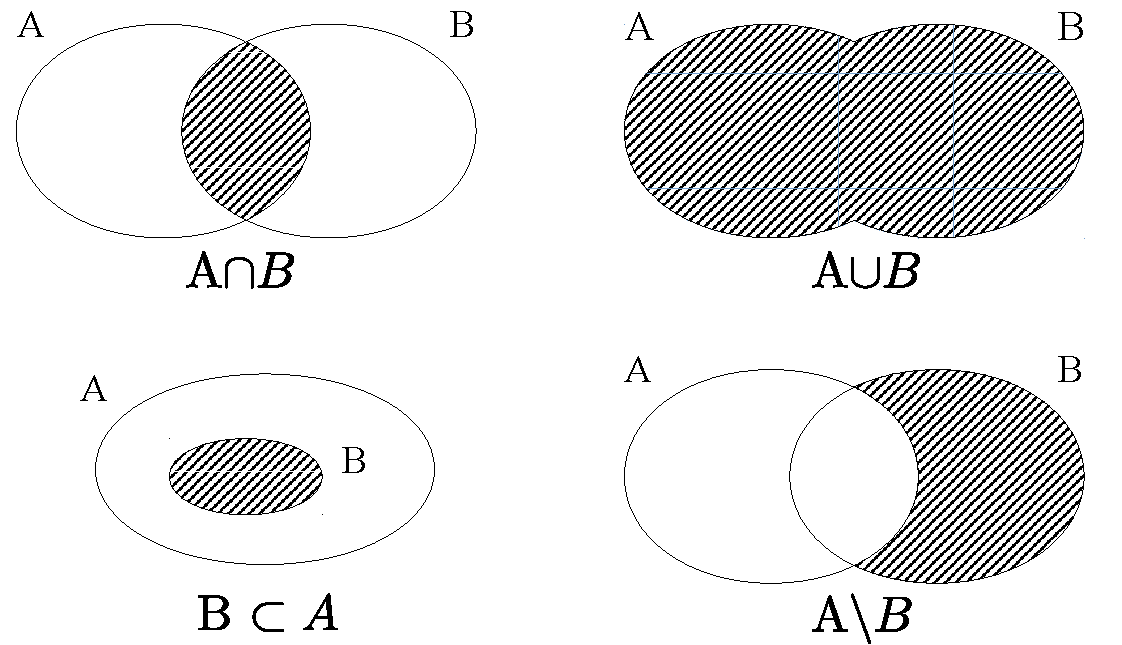
\includegraphics[width=0.7\textwidth, trim={0cm 0cm 0cm
          0cm},clip]{setRelations}
          \caption[]{}
          \label{fig: set relations}
        \end{figure}
      \subsection*{Maps}
        \begin{definition}[Maps between sets]
          Let $A$ and $B$ be two sets. A map $f$ is a many-to-one or
          one-to-one relation between elements in set $A$ and elements in set
          $B$. I.e, $\forall a \in A$, we have a corresponding element $f(a)
          \in B$. We denote a map in one of these two ways:
          \[A \xrightarrow{f} B \quad \quad f: A \rightarrow B\]
        \end{definition}
        \begin{definition}[Images and pre-images]
          Suppose we have $f: A\rightarrow B$. We say that $f(A)$ is the
          image of $A$ under $f$.\\
          We can also define a concept known as the pre-image of a map $f$,
          which we denote as $f^{-1}$. I.e, $\forall b \in B$, we have:
          $f^{-1}(b) = \{a \in A \,|f(a) = b\}$. Note that $f^{-1}$ is not necessarily a map, because $f^{-1}$ can be one-to-many.
        \end{definition}
        \begin{definition}(Injective, Surjective and Bijective)
          \begin{itemize}
            \item{A map $f: A \rightarrow B$ is one-to-one, or injective, if
            $\forall a,b \in A$, $f(a) = f(b) \Leftrightarrow a=b$.}
            \item{A map $f: A \rightarrow B$ is onto, or surjective, if
            $\forall b \in B$, $\exists a \in A$ such that $f(a) = b$. In other words, $f(A) = B$.}
            \item{A map $f: A \rightarrow B$ is bijective if and only if it is both surjective and injective.}
          \end{itemize}
        \end{definition}
        \subsubsection*{Inverse maps and composition of maps}
          Notice that if $f$ is bijective, then $\forall b \in B$, $f^{-1}(b)
          \equiv a \in A$ is a unique element such that $f(a) = b$. In other
          words, if $f$ is a bijective map from $A \rightarrow B$, then
          $f^{-1}$ is a map from $B \rightarrow A$ such that $f \circ f^{-1}$
          is the identity map from $B \rightarrow B$ and $f^{-1} \circ f$ is
          the identity map from $A \rightarrow A$. We call $f^{-1}$ the inverse
          map of $f$.

          Here we have also introduced the composition of two maps, denoted
          by $\circ$. I.e, if \[A \xrightarrow{f} B, B \xrightarrow{g} C\]
          then $g \circ f$ is a map from $A \rightarrow C$.
        \subsubsection*{Useful rules for maps}
          For maps in general, there are some useful rules which are listed below:
          \begin{enumerate}
            \item{Let $f: X\rightarrow Y$ be a map between two sets $X$ and
            $Y$. Then for any subsets $A,B$ of $X$, we can show that:
            \begin{itemize}
              \item{$f(A \cup B) = f(A) \cup f(B)$}
              \item{$f(A \cap B) \subset f(A) \cap f(B)$}
              \item{$f(A \backslash B) \supset f(A) \backslash f(B)$}
            \end{itemize}}
            \item{Let $f: X\rightarrow Y$ be a map between two sets $X$ and
            $Y$. Then for any subsets $A,B$ of $Y$, we can show that:
            \begin{itemize}
              \item{$f^{-1}(A \cup B) = f^{-1}(A) \cup f^{-1}(B)$}
              \item{$f^{-1}(A \cap B) = f^{-1}(A) \cap f^{-1}(B)$}
              \item{$f^{-1}(A \backslash B) = f^{-1}(A) \backslash f^{-1}(B)$}
            \end{itemize}}
          \end{enumerate}
          \begin{proof}
            \textcolor{red}{Coming soon! For now, see Kuldip's tutorial 1.
            This question is quite a standard math question in introductory
            math books...}
          \end{proof}
      \subsection*{Equivalence classes}
      Given a set $A$, we can define an equivalence relation $~$ between
      elements of the set like this: $\forall x,y \in A$, we write $x~y$ if
      $~$ satisfies the following three properties:
      \begin{enumerate}
        \item{Reflexive: $x\sim x$}
        \item{Symmetric: if $x\sim y$ then $y\sim x$}
        \item{Transitive: if $x\sim y$ and $y\sim z$ then $x\sim z$}
      \end{enumerate}
      \begin{theorem}[Fundamental theorem of equivalence relations]
        Let $\sim$ be an equivalence relation on the set $A$. If for every $x
        \in A$ we form the subsets \[B_x = \{y\in A \,|y\sim x\}\] then the
        family of subsets $B_x$ is a partition of $A$. The set $B_x$ is
        called an equivalence class with representative $x$. By partition, we
        mean that:
        \begin{enumerate}
          \item{$A = \bigcup\limits_{x\in A} B_x$}
          \item{If $B_x \cap B_y \neq \phi$ then $B_x = B_y$}
        \end{enumerate}
      \end{theorem}
      \begin{remark}
        By the way, we call the set of all equivalence classes,
        $\{B_x\}_{x\in A}$, denoted by $A\backslash \sim$, the quotient set.
      \end{remark}
      \begin{proof}
        \textcolor{red}{Will fill in soon. For now, just refer to any
        introductory math textbook... (Proof by reference)}
      \end{proof}
    \section{Basics of point-set Topology}
      \begin{definition}[Topology]
        \label{defn: defn of topology}
        A topological structure, or more briefly a topology, on a set $X$ is
        a structure given by a set $\mathcal{D}$ of subsets of $X$ having the
        following properties (called axioms of topological structures):
        \begin{enumerate}
          \item{Every union of sets of $\mathcal{D}$ is a set of
          $\mathcal{D}$}
          \item{Every finite intersection of sets of $\mathcal{D}$ is a set
          of $\mathcal{D}$ \label{item: topology defn axiom 2}}
        \end{enumerate}
      \end{definition}
      \begin{remark} A few remarks are in order:
        \begin{itemize}
          \item{When the cardinality of $X$ is countably/uncountably
          infinite, there might be some difficuly with axiom \ref{item:
          topology defn axiom 2}. This is a technical detail, not that
          important.}
          \item{It is easy to prove that $\phi$ and $X$ are always elements of
          $\mathcal{D}$.}
          \item{The power set $\mathcal{P}(X)$ of $X$ is an example of a
          topology on $X$. The trivial topology $\mathcal{D} = \{\phi, X\}$
          is also a topology on $X$. We can prove this by checking that both
          the power set and the trivial topology satisfies
          defintion~\ref{defn: defn of topology}.}
          \item{The set $X$ together with $\mathcal{D}$ is known as a
          topological space. The elements of $\mathcal{D}$ are known as the
          open sets of this topological space.}
        \end{itemize}
      \end{remark}
    \begin{definition}[Closed sets]
      Given a topological space $(X, \mathcal{D})$, closed sets are the
      complements of open sets.
    \end{definition}
    The above definition of closed sets is if we use definition~\ref{defn:
    defn of topology} as the definition of a topology. If we use
    definition~\ref{defn: alternate defn of topology} instead, then we will
    start with closed sets. Then, open sets would be defined as the
    complements of closed sets.
    \begin{definition}[Alternate definition of a topology]
      \label{defn: alternate defn of topology}
      An alternate definition of a topology can also be given in terms of
      closed sets: Consider the set $\mathcal{D}^\prime$ of subsets of $X$ with
      the following properties:
      \begin{enumerate}
        \item{Every finite union of sets in $\mathcal{D}^\prime$ is a set in
        $\mathcal{D}^\prime$}
        \item{Every intersection of sets in $\mathcal{D}^\prime$ is a set in
        $\mathcal{D}^\prime$}
      \end{enumerate}
      Note that here, $\phi$ and $X$ are also elements of
      $\mathcal{D}^\prime$. Elements of $ \mathcal{D}^\prime$ are known as
      closed sets, and then open sets can be defined as the complement of
      closed sets.
    \end{definition}
    \begin{definition}[Interior points, Exterior points, Boundary points]
      Consider a subset $A$ of a topological space $X$. We can characterise
      $x \in X$ as being either an interior point, exterior point or boundary
      point
      \textcolor{red}{Coming soon!}
    \end{definition}
    \subsection{Metric topology}
      \textcolor{red}{Coming soon!}
    
    \chapter{Manifolds and Coordinates}
  \begin{definition}[$C^k$ Functions]
    A function $f: \mathbb{R}^n\rightarrow \mathbb{R}^n$ is said to be in $C^k$ if all its partial derivatives up to and including order $k$ exist and are continuous.
  \end{definition}
  \begin{remark}
    When $k\rightarrow \infty$, the function $f: \mathbb{R}^n\rightarrow \mathbb{R}^n$ is said to be smooth, or in $C^{\infty}$.
  \end{remark}
  \section{Topological and Differentiable Manifolds}
    \begin{definition}[Topological Manifold\footnote{For a precise meaning
    of the terms "Hausdorff","Neighbourhood", "Homeomorphic", wait for
    chapter \ref{chapter:Basic Topology} to be done.}]
      A topological manifold is a Hausdorff space such that every point has a
      neighbourhood homeomorphic to $\mathbb{R}^n$.
    \end{definition}
    \begin{remark}
      A manifold that is locally homeomorphic to $\mathbb{R}^n$ is said to have dimension $n$.
    \end{remark}
    Since every point on the manifold has a neighbourhood homeomorphic to
    $\mathbb{R}^n$, locally the neighbourhood on the manifold "inherits"
    the metric topology of $\mathbb{R}^n$. I.e, the local homeomorphism to
    $\mathbb{R}^n$ implies the existence of open sets on the manifold, and
    because a homeomorphism is by definition bijective, there is a
    one-to-one correspondence between open sets in the neighbourhood and
    open sets in $\mathbb{R}^n$.

    In short, "locally" (in the neighbourhood of a point), the manifold has
    the same topology as $\mathbb{R}^n$.

    By the way, the manifold "inheriting" the metric topology of
    $\mathbb{R}^n$ locally is a very different concept from the idea of a
    metric tensor. So far, no metric has been defined on the manifold yet!

  \section{Charts}
    \begin{definition}[Chart]
      A chart $(U, \phi)$ of a manifold $\mathcal{M}$ is an open set U of $\mathcal{M}$, called the domain of the chart, together with a homeomorphism $\phi: U \rightarrow V$ of $U$ onto an open set $V$ in $\mathbb{R}^n$
    \end{definition}
    I.e, for an arbitrary $p\in U \subset \mathcal{M}$, we have $\phi(p) =
    \left(x^1(p), x^2(p),...,x^n(p)\right) \in \mathbb{R}^n$. We say that
    $p \in U$ has coordinates $\phi(p)$ in the chart $(U, \phi)$.

    In Physics terms, we would call $\left\{x^i(p)\right\}_{i = 1,...n}$
    the coordinate functions, and we would call the chart $(U, \phi)$ a
    local coordinate system.
  \section{Atlas}
    \begin{definition}[Atlas]
      \label{defn: Atlas definiton}
      An atlas of class $C^k$ on a manifold $\mathcal{M}$ is a set (i.e
      family) $\{(U_\alpha,\phi_\alpha)\}_{\alpha \in I}$\footnote{Note
      that $I\subset \mathbb{R}$} of charts of $\mathcal{M}$ such that the
      following holds:
      \begin{enumerate}
        \item{M is covered by the family in the sense that
          \begin{equation*}
            \mathcal{M} = \bigcup_{\alpha\in I} U_\alpha
          \end{equation*}}
        \item{\label{item:atlas defn}The maps $\phi_\beta \circ
        \phi_\alpha^{-1}: \phi_\alpha(U_\alpha \cap U_\beta) \rightarrow
        \phi_\beta(U_\alpha \cap U_\beta)$ are maps of open sets of
        $\mathbb{R}^n$ into $\mathbb{R}^n$ of class $C^k$.}
      \end{enumerate}
    \end{definition}
      Let's spend more time looking at property \ref{item:atlas defn} of
      defintion \ref{defn: Atlas definiton}.
      \begin{figure}[ht]
        \centering
        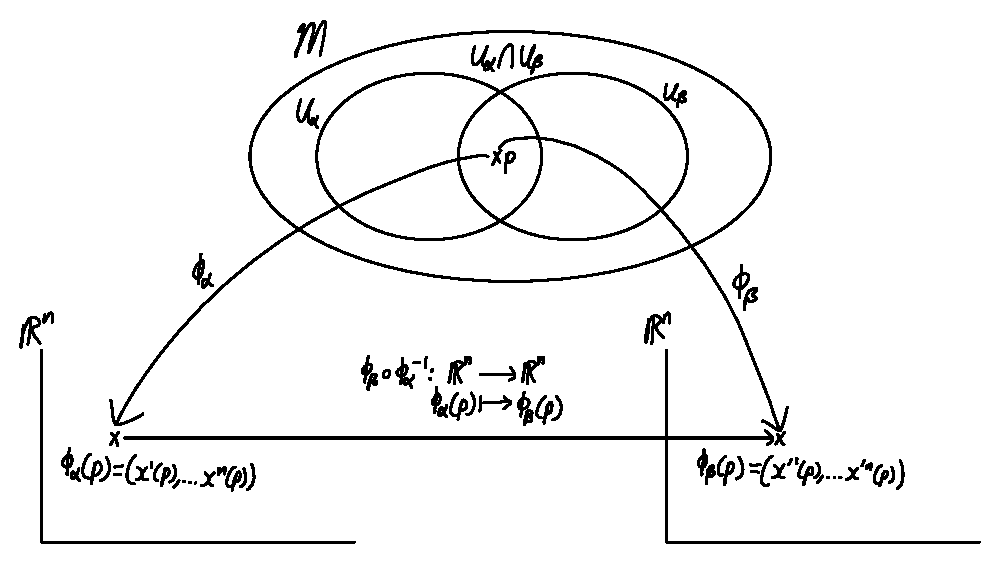
\includegraphics[width=0.7\textwidth, trim={0cm 0cm 0cm 0cm},clip]{Atlas defn}
        \caption[]{}
        \label{fig:atlas defn}
      \end{figure}
      With reference to Figure~\ref{fig:atlas defn}, consider a point $p
      \in U_\alpha \cap U_\beta$. $p$ has coordinates $\phi_\alpha(p)$ in
      the chart $(U_\alpha,\phi_\alpha)$, but has coordinates
      $\phi_\beta(p)$ in the chart $(U_\beta,\phi_\beta)$. These two charts
      induce a map\footnote{$\phi_\alpha^{-1}$ exists because $\phi_\alpha$ is a homeomorphism.} $\phi_\beta \circ \phi_\alpha^{-1}$ from
      $\phi_\alpha(U_\alpha \cap U_\beta) \subset \mathbb{R}^n$ to
      $\phi_\beta(U_\alpha \cap U_\beta) \subset \mathbb{R}^n$. Now, the
      map $\phi_\beta \circ \phi_\alpha^{-1}$ is actually $n$ coordinate
      transformation functions $\{x^{\prime i} = x^{\prime
      i}(x^1,...,x^n)\}_{i=1,...n}$. Thus, when we say that the map
      $\phi_\beta \circ \phi_\alpha^{-1}$ is of class $C^k$, we are saying
      that those $n$ coordinate transformation functions are also of class
      $C^k$.

      Two charts $(U_\alpha,\phi_\alpha)$, $(U_\beta,\phi_\beta)$ that satisfy the property are said to be $C^k$ compatible.

      \begin{definition}[Equivalent Atlases]
        Two $C^k$ atlases $\mathcal{F} = \{(U_\alpha,\phi_\alpha)\}_{\alpha
        \in I}$ and $\mathcal{G} =
        \{(U_{\alpha^\prime},\phi_{\alpha^\prime})\}_{\alpha^\prime \in I}$
        are equivalent\footnote{"Equivalent" here refers to equivalence relation, so we can form equivalence classes.} if every pair of charts $(U_\alpha,\phi_\alpha) \in
        \mathcal{F}$ and $(U_{\alpha^\prime},\phi_{\alpha^\prime}) \in
        \mathcal{G}$ are $C^k$ compatible.
      \end{definition}
      \begin{remark}
        An equivalent definiton (can be proved) is: Two $C^k$ atlases $\mathcal{F} = \{(U_\alpha,\phi_\alpha)\}_{\alpha
        \in I}$ and $\mathcal{G} =
        \{(U_{\alpha^\prime},\phi_{\alpha^\prime})\}_{\alpha^\prime \in I}$
        are equivalent if their union $\mathcal{F} \cup \mathcal{G}$ is a $C^k$ atlas.
      \end{remark}
  \section{Differentiable Manifold}
    \begin{definition}[Differentiable Manifold]
      A topological manifold $\mathcal{M}$ together with an equivalence
      class of $C^k$ atlases is a $C^k$ structure on $\mathcal{M}$; we say
      that $\mathcal{M}$ is a $C^k$ manifold or a differentiable manifold.
    \end{definition}
    \begin{remark}
      Very often, we want $k \rightarrow \infty$, so we can define tensor
      fields on $\mathcal{M}$. In this case, the manifold is called a smooth manifold.
    \end{remark}
  \section{Key Idea Behind Differential Geometry}
    In Physics, most of the time the variables that we are concerned with
    such as time, position, etc are all either elements of $\mathbb{R}$
    or $\mathbb{C}$, and our physical laws themselves are usually
    differential equations. Yet we know that the laws of Physics are
    independent of the choice of coordinates used. Thus, differential
    geometry is a natural language for expressing the laws of Physics.
    When we model our physical system with a differentiable manifolds, we
    can do calculus because locally the manifold looks like
    $\mathbb{R}^n$. But our results are also coordinate independent,
    because we can freely switch between coordinates due to the $C^k$
    structure; we just have to use the chain rule to do so.

    By the way, from here on, we deal strictly with differentiable or smooth manifolds.
  \section{Diffeomorphisms}
    \label{sec: Diffeomorphism}
    \begin{definition}[Differentiable Maps between Manifolds]
      \label{defn: differentiable map}
      Let $\mathcal{M}$, $\mathcal{N}$ be two $C^k$ differentiable
      manifolds of dimensions $m$ and $n$ respectively. Let $\mathcal{M}$
      have an atlas $\{(U_\alpha, \phi_\alpha)\}_{\alpha\in I}$\footnote{We
      will slowly drop the $"\alpha\in I"$ label for ease of notation...},
      and $\mathcal{N}$ have an atlas $\{(V_\beta, \psi_\beta)\}_{\beta\in
      I}$. Let $f$ be a map from $\mathcal{M}$ to $\mathcal{N}$.
      
      The map $f$ is said to be $C^r$ differentiable at $p\in\mathcal{M}$,
      $r\leq k$ if the $n$ coordinate transforms induced by $F \equiv \psi
      \circ f \circ \phi^{-1}$ are $C^r$ differentiable at $\phi(p)$, where
      $(U,\phi) \in \{(U_\alpha, \phi_\alpha)\}$ is a chart such that $p
      \in U$ and $(V,\psi) \in \{(V_\beta, \psi_\beta)\}$ is a chart such
      that $f(p) \in V$.
      
      If $f$ is differentiable $\forall p \in \mathcal{M}$, then $f$ is a
      differentiable map.
    \end{definition}
    \begin{remark}
      In definition~\ref{defn: differentiable map}, two particular charts
      $(U,\phi)$, $(V,\psi)$ are chosen. Yet it doesn't matter which charts
      we choose. Consider two other charts $(U^\prime,\phi^\prime)$ and
      $(V^\prime,\psi^\prime)$ such that $p \in U^\prime$, $f(p) \in
      V^\prime$. Consider $F^\prime = \psi^\prime \circ f \circ
      \phi^{\prime -1}$. Note that we can write\footnote{This trick of
      inserting an identity map $(\psi^{-1} \circ \psi)$ is a very useful
      trick, especially in proofs.} $F^\prime = \psi^\prime \circ
      (\psi^{-1} \circ \psi) \circ f \circ (\phi^{-1} \circ \phi) \circ
      \phi^{\prime -1} = (\psi^\prime \circ \psi^{-1}) \circ F \circ (\phi
      \circ \phi^{\prime -1})$, and because of the $C^k$ structure of the
      differentiable manifold, both $(\psi^\prime \circ \psi^{-1})$ and
      $(\phi \circ \phi^{\prime -1})$ are both $C^k$ functions. Thus, if
      $F$ is a $C^r$ function, then $F^\prime$ is also a $C^r$ function.
    \end{remark}
    \begin{figure}[h]
      \centering
      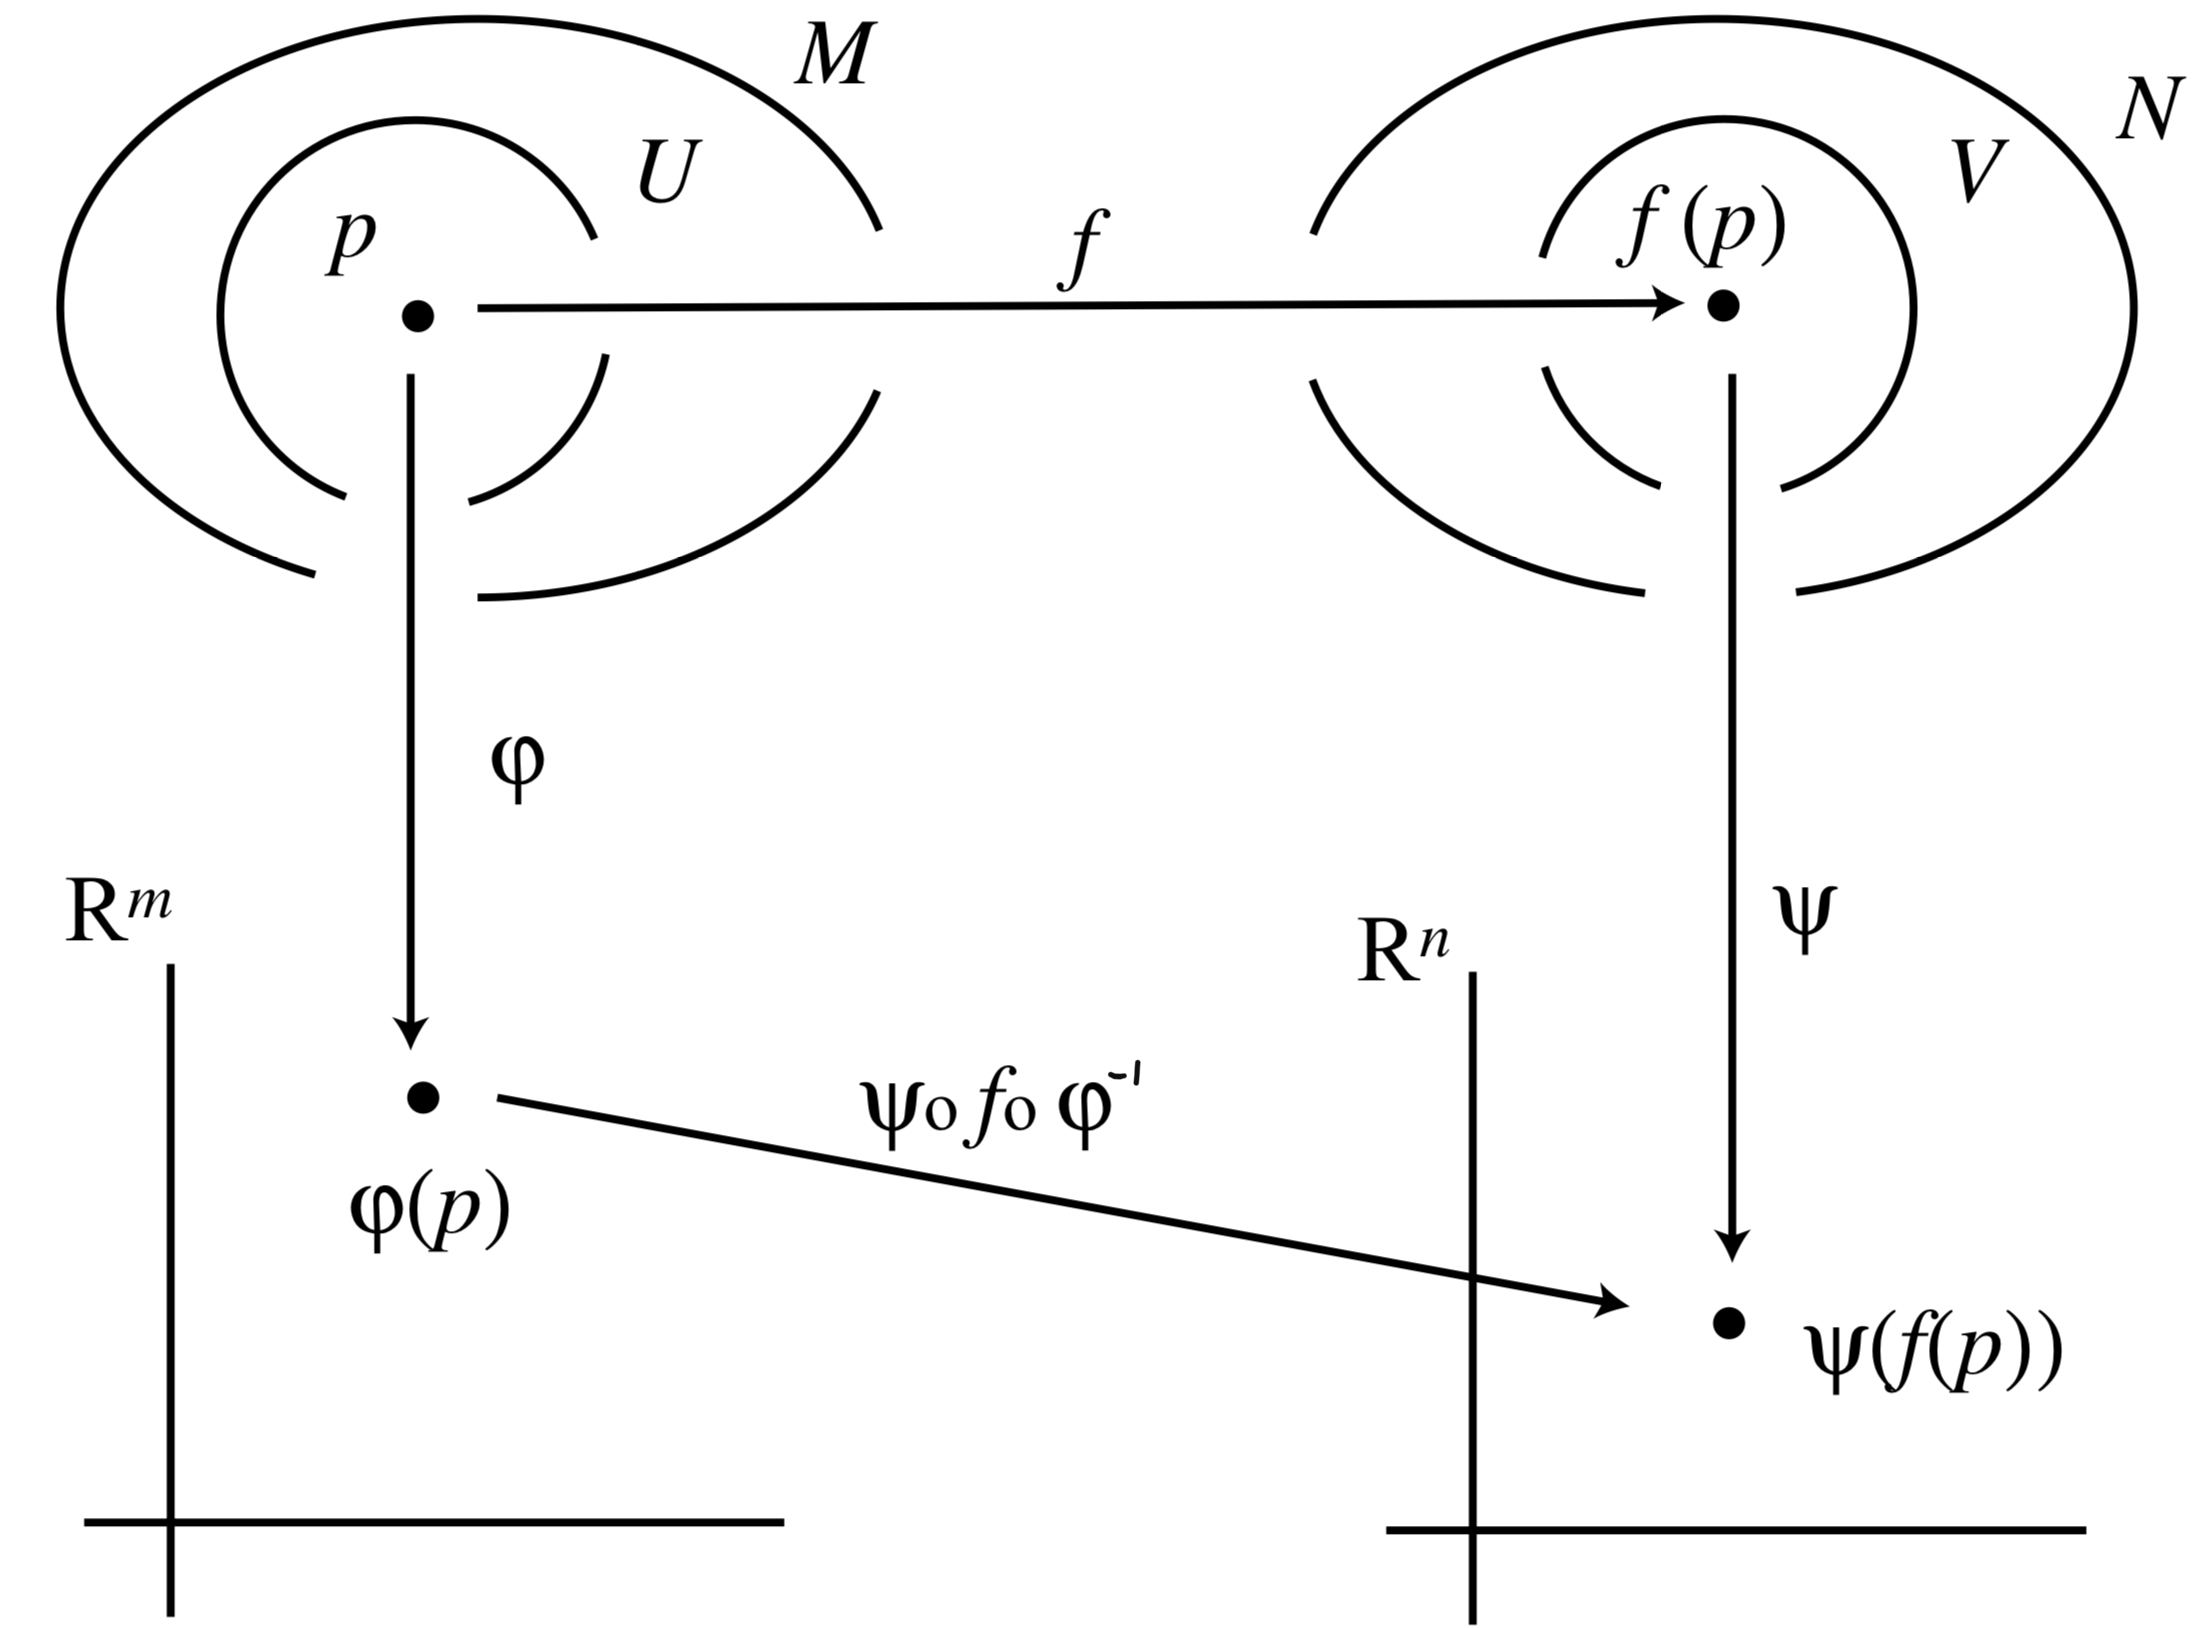
\includegraphics[width=0.6\textwidth, trim={0cm 0cm 0cm 0cm},clip]{Differentiable Map defn}
      \caption[]{Figure copied from Nakahara}
      \label{fig: differentiable map defn}
    \end{figure}
    Let's try to make sense of the above definition. With reference to
    Figure~\ref{fig: differentiable map defn}, consider a point $p\in
    \mathcal{M}$ and its image under $f$, i.e $f(p) \in \mathcal{N}$.
    Consider two charts, $(U,\phi) \in \{(U_\alpha, \phi_\alpha)\}$ and
    $(V,\psi) \in \{(V_\beta, \psi_\beta)\}$ such that $p \in U$ and $f(p)
    \in V$. Then, $F = \psi \circ f \circ \phi^{-1}$ is a map from $\phi(U)
    \subset \mathbb{R}^n$ to $\psi(V)\subset \mathbb{R}^m$. In fact, we see
    that $F$ induces $n$ coordinate transformation functions; if we let
    $\phi(p) = \left(x^1,...,x^m\right)$, then $\psi(f(p)) =
    \left(x^{\prime 1},...x^{\prime n}\right) = \left(x^{\prime
    1}(x^1,...,x^m),...x^{\prime n}(x^1,...,x^m)\right)$. Then, for $f$ to be a differentiable map, these $n$ coordinate functions have to be $C^r$.
    \begin{definition}[Diffeomorphism]
      A map $f:\mathcal{M} \rightarrow \mathcal{N}$, where $\mathcal{M}$ and
      $\mathcal{N}$ are $C^k$-differentiable manifolds of dimensions $m$ and
      $n$ respectively, is said to be a diffeomorphism if:
      \begin{enumerate}
        \item{$f$ is bijective $(\implies m = n)$.}
        \item{$f$ and $f^{-1}$ are both $C^r$ functions.}
      \end{enumerate}
    \end{definition}
    \chapter{Tangent Spaces}
  \section{Curves and Functions on a Manifold}
    \begin{definition}[Curve on a Manifold]
      A (parametrized) curve $\sigma$ on a m-dimensional manifold
      $\mathcal{M}$ is an injective map from $I\subset \mathbb{R}$ into
      $\mathcal{M}$ by:
      \begin{equation*}
        t\in I \rightarrow \sigma(t) \in \mathcal{M}
      \end{equation*}
    \end{definition}
      The curve is also said to be differentiable if the map $\sigma$ is
      differentiable.
    \begin{definition}[Differentiable Curve on a Manifold]
      The idea of $\sigma$ being differentiable is defined as follows:
      Consider a chart $(U, \phi)$ that covers the entire curve, i.e
      $\sigma(I) \subset U$. Then, $\sigma$ being differentiable is defined
      as the map $\bar{\sigma} \equiv \phi \circ \sigma$ from $I$ to
      $\mathbb{R}^m$ being differentiable.

      Note that $\bar{\sigma}(t) = \left(x^1(t),...x^m(t)\right)$, thus
      $\bar{\sigma}$ being differentiable means that the $m$ coordinate
      functions ${x^i(t)}$ are differentiable with respect to $t$. 

      Note also that the differentiability of $\sigma$ is coordinate
      independent, as can be easily proved by considering another chart
      $(V,\psi)$ that covers the entire curve, and noting that if $\phi
      \circ \sigma$ is differentiable, then so is $\psi \circ \sigma$
      because:
      \begin{equation}
        \label{eqn: cheap trick coordinate independence}
        \psi \circ \sigma = \underbrace{\psi \circ \phi^{-1}}_{\in C^k}
        \circ  \, \, \phi \circ \sigma
      \end{equation}
    \end{definition}
    \begin{remark}
      Equation~\ref{eqn: cheap trick coordinate independence} is an example
      of a really useful trick, where we insert an identity map $\phi^{-1}
      \circ \phi$ or $\phi \circ \phi^{-1}$ to show that certain things are
      independent of the chart chosen. In fact, we have seen something like
      this in section~\ref{sec: Diffeomorphism}. We will use this trick
      frequently, but from now on, we will not show the explicit calculation, but only make a brief comment.
    \end{remark}
    \begin{definition}[Function on a Manifold]
      A function $f$ on a manifold $\mathcal{M}$ is the map $f:\mathcal{M}
      \rightarrow \mathbb{R}$.
    \end{definition}
    \begin{definition}[$C^r$Function on a Manifold]
      A function $f$ on a manifold $\mathcal{M}$ is said to be $C^r$ at $p
      \in \mathcal{M}$ if in a chart $(U,\phi)$ such that $p\in U$,
      $\bar{f} \equiv f \circ \phi^{-1}$ is a $C^r$ function from
      $\mathbb{R^m}$ to $\mathbb{R}$.

      Note that the above defintion can be shown to be independent of the
      choice of chart $(U,\phi)$; we can consider another chart $(V, \psi)$
      and do the insertion of identity trick as was done in
      equation~\ref{eqn: cheap trick coordinate independence}.

      If $f$ is $C^r \,\, \forall p \in \mathcal{M}$, then we say that $f \in
      C^r(\mathcal{M})$, or that $f$ is a $C^r$ function on the manifold
      $\mathcal{M}$.
    \end{definition}
    \subsection{Useful notation: Overbar}
      The astute reader might have noticed by now that we have been quite
      consistent in our notation, in where we place an overbar.
      Specifically, for some chart $(U,\phi)$ we have done:
      \begin{itemize}
        \item{$f:\mathcal{M}\rightarrow \mathbb{R}$ leads to $\bar{f} \equiv f \circ \phi:\mathbb{R}^m \rightarrow \mathbb{R}$}
        \item{$\sigma:I \subset \mathbb{R} \rightarrow \mathcal{M}$ leads to
        $\bar{\sigma}\equiv \phi \circ \sigma: \mathbb{R} \rightarrow \mathbb{R}^m$}
      \end{itemize}
      Thus, for any map that involves a manifold $\mathcal{M}$, we shall
      use the overbar to denote its representation in some local coordinate
      system (i.e, in some chart). Some examples (including those which we will see later):
      \begin{itemize}
        \item{$f:\mathcal{M}\rightarrow \mathcal{N}$ leads to $\bar{f} =
        \phi^{-1}\circ f \circ \psi: \mathbb{R}^m \rightarrow \mathbb{R}^n$
        where $(U,\phi)$ is some chart in $M$, $(V,\psi)$ is some chart in
        $N$.}
        \item{$X: C^\infty(\mathcal{M})\rightarrow C^\infty(\mathcal{M})$
        leads to $\bar{X}:C^\infty(\mathbb{R}^m)\rightarrow
        C^\infty(\mathbb{R}^m)$}
      \end{itemize}
  \section{Tangent Vectors}
    \begin{definition}[Tangent Vector to a Curve]
      The tangent vector to a curve $\sigma$ at some point $p\in
      \mathcal{M}$ is defined:
      \begin{equation*}
        V^{\sigma}_{p}(f) = \frac{d}{dt}(f\circ\sigma)(t)\Bigr|_{t=0},
        \quad \sigma(0) = p
      \end{equation*}
      $\forall f \in C^k(\mathcal{M})$.
    \end{definition}
    Note that $V^{\sigma}_{p}(f)$ is a number. Now, there could be multiple
    curves with the same tangent vector; for example in $\mathbb{R}^2$, the
    curves $\sigma_1(t) = (t,e^t)$ and $\sigma_2(t) = (t, 1 + t)$ are
    tangent at $p = (1,1)\in \mathbb{R}^2$. Let's extend this idea to a
    general manifold $\mathcal{M}$.
    \begin{definition}[Two curves being tangent at $p\in \mathcal{M}$]
      \label{defn: two curves being tangent}
      Two curves on the manifold $\mathcal{M}$, $\sigma_1(t)$ and
      $\sigma_2(t)$, are said to be tangent at $\sigma_1(0) = \sigma_2(0) =
      p \in \mathcal{M}$ if for all $f \in C^k(\mathcal{M})$, the following
      holds:
      \begin{equation*}
        \frac{d}{dt}(f\circ \sigma_1)(t)\Bigr|_{t=0} = \frac{d}{dt}(f\circ
        \sigma_2)(t)\Bigr|_{t=0}
      \end{equation*}
    \end{definition}
    \begin{remark}
      The $\sigma_1(0) = \sigma_2(0) = p \in \mathcal{M}$ condition is just
      saying that the two curves must intersect. Without loss of
      generality, if $\sigma_1(t_1) = \sigma_2(t_1) = p \in \mathcal{M}$
      and $\frac{d}{dt}(f\circ \sigma_1)(t)|_{t=t_1} =
      \frac{d}{dt}(f\circ \sigma_2)(t)|_{t=t_1}$ for some $t_1\in
      \mathbb{R}$, then we can just do a change of variables $t = t + t_1$
      to recover our original definition. I.e, definition \ref{defn: two
      curves being tangent} is general enough.
    \end{remark}
    \begin{remark}
      In other words, two curves $\sigma_1(t)$ and $\sigma_2(t)$ are said
      to be tangent at $p\in \mathcal{M}$ if they have the same tangent
      vector at point $p\in \mathcal{M}$, i.e $V_p^{\sigma_1} =
      V_p^{\sigma_2}$. We will see what this means in more detail when we
      go into a local chart $(U,\phi)$.
    \end{remark}
    \subsection{Tangent vectors to a curve in a local chart $(U,\phi)$}
      This concept is very important and thus deserves a section of its
      own. Consider $p\in \mathcal{M}$, and a local chart $(U,\phi)$ around
      $p$, i.e $p\in U$. Consider also a curve $\sigma$ such that
      $\sigma(0)= p$.
      Then, we have:
        \begin{align*}
          V^{\sigma}_{p}(f) &= \frac{d}{dt}(f\circ\sigma)(t)\Bigr|_{t=0} \\
          &= \frac{d}{dt}(f\circ\phi^{-1}\circ \phi \circ
          \sigma)(t)\Bigr|_{t=0} \\
          &= \frac{d}{dt}(\bar{f}\circ\bar{\sigma})(t)\Bigr|_{t=0}
        \end{align*}
      where $\bar{\sigma}(t) = \left(x^1(t),...,x^m(t)\right)$ is a curve
      in $\mathbb{R}^m$, and $\bar{f}$ is a map from $\mathbb{R}^m$ to
      $\mathbb{R}$. Continuing with our calculation, we have:
        \begin{align*}
          V^{\sigma}_{p}(f)
          &=\frac{d}{dt}(\bar{f}\circ\bar{\sigma})(t)\Bigr|_{t=0} \\
          &=\frac{d}{dt}\bar{f}(x^1(t),...,x^m(t))\Bigr|_{t=0}\\
          &=\frac{dx^i}{dt}\Bigr|_{t=0}\frac{\partial \bar{f}}{\partial
          x^i}\Bigr|_{\phi(p)} \\
          &=\frac{dx^i}{dt}\Bigr|_{t=0}\frac{\partial}{\partial x^i}(\bar{f})
        \end{align*}
      where in the last line, we write $\frac{\partial \bar{f}}{\partial
      x^i}\Bigr|_{\phi(p)}$ as $\frac{\partial \bar{f}}{\partial x^i}$ for
      ease of notation, as we will sometimes do in the future. Now, since
      the above calculations are true for all $f \in C^k(\mathcal{M})$, we
      have:
      \begin{equation}
        \label{eqn: tangent vector to a curve in local coords}
        V^{\sigma}_{p} \xrightarrow{\text{local chart}}
        \frac{dx^i}{dt}\Bigr|_{t=0}\frac{\partial}{\partial x^i}
      \end{equation}
      Equation~\ref{eqn: tangent vector to a curve in local coords} tells
      us what it means for two curves $\sigma_1(t)$ and $\sigma_2(t)$ to be
      tangent at $p\in\mathcal{M}$. In a local chart $(U,\phi)$,
      $\sigma_1(t)$ and $\sigma_2(t)$ are tangent at $p\in\mathcal{M}$ if and only if these two conditions hold:
      \begin{enumerate}
        \item{$\sigma_1(0) = \sigma_2(0) = p$}
        \item{\label{item: tangent condition}If we write $\bar{\sigma_1}(t)
        = \left(x^1(t),...,x^m(t)\right)$ and $\bar{\sigma_2}(t) =
        \left(x^{\prime 1}(t),...,x^{\prime m}(t)\right)$, then
        \begin{equation*}
          \frac{dx^i}{dt}\Bigr|_{t=0} = \frac{dx^{\prime i}}{dt}\Bigr|_{t=0}
        \end{equation*}}
        for all $i = 1,...,m$.
      \end{enumerate}
    By the way, it can be proven\footnote{Refer to Kuldip's tutorials, or
    Nakahara/Frankel} that if condition~\ref{item: tangent condition} is
    true in one local chart $(U,\phi)$, then it is true for all charts. 
    
    \subsection{Motivating the definition of a tangent vector at a point}
      So far, we have defined a tangent vector to a curve. However, the
      above calculation explicitly shows us that we cannot identify tangent
      vectors uniquely with curves, since there could be many different
      curves that give the same tangent vector.
      
      However, if we take the set of all curves that pass through a point
      $p\in \mathcal{M}$, and separate them into equivalence classes where
      the equivalence relation between two curves is that they are tangent
      at the point $p\in \mathcal{M}$, then we can uniquely identify
      different tangent vectors with different equivalence classes of
      curves. This is what we will do.

    \begin{definition}[Tangent Vector at a point $p \in \mathcal{M}$]
      \label{defn: Tangent vector at a point}
      A tangent vector at $p \in \mathcal{M}$, $V^{\sigma}_{p}$ is defined
      as \begin{equation*}
          V^{\sigma}_{p}(f) = \frac{d}{dt}(f\circ\sigma)(t)\Bigr|_{t=0},
          \quad \sigma(0) = p
        \end{equation*}
      $\forall f\in C^k(\mathcal{M})$, where $\sigma$ is any representative
      of an equivalence class of curves, denoted $[\sigma]_p$. The
      equivalence relation between two curves is that they are tangent at
      the point $p\in \mathcal{M}$.
    \end{definition}
    \begin{remark}
      Sometimes, we write $V^{\sigma}_{p} = [\sigma]_p$, i.e we identify
      the tangent vector directly with the equivalence class of curves that
      it is defined with. Recall: different equivalence class of curves
      $\implies$ different tangent vectors!

      In fact, we will do this a lot in this set of notes; this is a convention inherited from Kuldip.
    \end{remark}
    \subsection{Tangent vectors at a point $p\in\mathcal{M}$ in a local
    chart $(U,\phi)$}
      The local representation of a tangent vector at a point,
      $V^{\sigma}_{p}$, is exactly the same the local representation of a
      tangent vector to a curve, given in equation~\ref{eqn: tangent vector
      to a curve in local coords}. The only difference is that the term
      $\frac{dx^i}{dt}\Bigr|_{t=0}$ is now uniquely identified with an
      equivalence class of curves $[\sigma]_p$. Let's reproduce
      equation~\ref{eqn: tangent vector to a curve in local coords} here
      for convenience:
      \begin{equation*}
        V^{\sigma}_{p} \xrightarrow{\text{local chart}}
        \frac{dx^i}{dt}\Bigr|_{t=0}\frac{\partial}{\partial x^i}
      \end{equation*} Now, we can write $V^i \equiv
      \frac{dx^i}{dt}\Bigr|_{t=0}$, and call $V^i$ the components of the
      vector $V^{\sigma}_{p}$ in a local chart $(U,\phi)$. Then, we have:
      \begin{equation}
        \label{eqn: Tangent vector to a point local coord}
        V^{\sigma}_{p} \xrightarrow{\text{local chart}} V^i
        \frac{\partial}{\partial x^i} = V^i \partial_i
      \end{equation}
      From equation~\ref{eqn: Tangent vector to a point local coord}, we
      also see that $V^{\sigma}_{p}$ is associated with a directional
      derivative in a local coordinate chart. This is the breakthrough of
      modern differential geometry, to associate tangent vectors to a point
      in the manifold with a directional derivative in $\mathbb{R}^m$. Note
      that because $V^{\sigma}_{p}$ is associated with a directional
      derivative, we have the Leibniz product rule. We will revisit this idea again when we talk about derivations.

      Lastly, we shall call the $m$ objects $\{\partial_i\}_{i=1,...,m}$
      the coordinate basis vectors to the tangent space $T_p(\mathcal{M})$.
      But let's not get ahead of ourselves, and revisit this idea again
      later when we formally develop the tangent space.

      Note that from here on, whenever we say "tangent vector", we are
      referring to tangent vectors at a point. Also, from
      definiton~\ref{defn: Tangent vector at a point}, we see that a local
      chart is unnecessary to define a tangent vector; local charts are
      used just for our convenience, when we want to do computations.
    \subsection{Transformation properties of the components of a tangent
    vector when we switch local charts}
      Since tangent vectors exist independently of any local charts, lets
      see how the components of the tangent vector $V^\sigma_p$ in a local
      chart $(U,\phi)$ are related to the components in another local chart
      $(U^\prime, \phi^\prime)$.

      Consider $f\in C^k(\mathcal{M})$. Then, in the local chart
      $(U,\phi)$, we have:
      \begin{equation*}
        V^\sigma_p(f) = V^i \left(\frac{\partial}{\partial x^i}
        \bar{f}(x^1,...,x^m)\right)\Bigr|_{\phi(p)}
      \end{equation*}
      where $\bar{f} = f \circ \phi^{-1}$.
      On the other hand, in the other local chart $(U^\prime,\phi^\prime)$,
      we have:
      \begin{equation*}
        V^\sigma_p(f) = V^{\prime i} \left(\frac{\partial }{\partial x^{\prime
        i}}\bar{f^\prime}(x^{\prime 1},...,x^{\prime m})\right)\Bigr|_{\phi^\prime(p)}
      \end{equation*}
      where $\bar{f^\prime} = f \circ \phi^{\prime-1}$.
      Note that $\bar{f}(x^1,...,x^m) = \bar{f^\prime}(x^{\prime
      1},...,x^{\prime m}) = f(p)$.

      But $\phi^{\prime} \circ \phi^{-1}$, a map from $\phi(U\cap U^\prime)
      \subset \mathbb{R}^m$ to $\phi^\prime(U\cap U^\prime) \subset
      \mathbb{R}^m$, induces $m$ coordinate transformation functions
      $\left\{x^{\prime i}(x^1,...,x^m)\right\}_{i=1,...,m}$. Thus, using the chain rule, we have:
      \begin{align*}
        \left(\frac{\partial}{\partial x^i}
        \bar{f}(x^1,...,x^m)\right)\Bigr|_{\phi(p)} 
        &= \left(\frac{\partial}{\partial x^i} \bar{f^\prime}(x^{\prime
        1}(x^1,...,x^m),...,x^{\prime m}(x^1,...,x^m))\right)
        \Bigr|_{\phi(p)}\\
        &= \frac{\partial x^{\prime j}}{\partial x^i}\Bigr|_{\phi(p)}
        \left(\frac{\partial }{\partial x^{\prime
        j}}\bar{f^\prime}(x^{\prime 1},...,x^{\prime
        m})\right)\Bigr|_{\phi^\prime(p)}
      \end{align*}
      Thus, substituting the chain rule calculation above into the
      expression for $V_p^\sigma(f)$ in the local chart $(U,\phi)$, we
      have:
      \begin{equation*}
        V^\sigma_p(f) = V^i \frac{\partial x^{\prime j}}{\partial
          x^i}\Bigr|_{\phi(p)} \left(\frac{\partial }{\partial x^{\prime
          j}}\bar{f^\prime}(x^{\prime 1},...,x^{\prime
          m})\right)\Bigr|_{\phi^\prime(p)}
      \end{equation*}
      which, when we compare with the expression for $V_p^\sigma(f)$ in the
      local chart $(U^\prime,\phi^\prime)$, we get:
      \begin{equation}
        \label{eqn: Tangent vector component contravariant transformation}
        V^{\prime i} = V^i \frac{\partial x^{\prime j}}{\partial
        x^i}\Bigr|_{\phi(p)}
      \end{equation}
      Thus, we note that the components of the tangent vector in a local
      coordinate chart transforms contravariantly under a change of
      coordinates! This contravariant transformation is a direct
      consequence of the identification of tangent vectors with directional
      derivatives in a local coordinate chart.
    \subsection{Tangent vectors as derivations}
      From definiton~\ref{defn: Tangent vector at a point}, we see that
      $V_p^\sigma$ is really a map from $C^k(\mathcal{M}) \rightarrow
      \mathbb{R}$. In fact, since
      \[V_p^\sigma(f) = V^i \frac{\partial\bar{f}}{\partial x^i}\]
      in a local chart $(U,\phi)$, where $\bar{f} = f\circ \phi^{-1}$,we
      have the following few properties:
      \begin{enumerate}
        \item{$V_p^\sigma(f+g) = V_p^\sigma(f) + V_p^\sigma(g) \quad
        \forall f \in C^k(\mathcal{M})$}
        \item{$V_p^\sigma(\alpha f) = \alpha V_p^\sigma(f) \quad \forall
        \alpha\in\mathbb{R} \text{ and } \forall f \in C^k(\mathcal{M})$}
        \item{$V_p^\sigma(f\cdot g) = g(p)V_p^\sigma(f) + f(p)V_p^\sigma(g)
        \quad \forall f,g\in C^k(\mathcal{M})$}
      \end{enumerate}
      Thus, $V^\sigma_p$ is something we call a derivation, which is a
      fancy name for a generalised derivative operator that satisfies the
      three properties above (and especially Leibniz's product rule).
  \section{The Tangent Space \texorpdfstring{$T_p(\mathcal{M})$}{Tp(M)}}
    \subsection{Constructing the Tangent Space $T_p(\mathcal{M})$}
      Here, we want to show that the set of all tangent vectors at a point
      $p\in \mathcal{M}$, which we denote as $\{V_p^\sigma\}$, has a vector
      space structure. 

      To do so, we first need to define the addition between two tangent
      vectors $V^{\sigma_1}_p = [\sigma_1]$ and $V^{\sigma_2}_p =
      [\sigma_2]$. Since tangent vectors are identified uniquely with
      equivalence classes of curves, if we could take the two equivalence
      classes of curves and produce a third equivalence class of curves, then
      we would have produced another tangent vector. Note that it is possible
      for $[\sigma_1] = [\sigma_2]$, in which case our result will still be
      in the same equivalence class as $[\sigma_1]$ (i.e, adding of two
      parallel vectors will give a third parallel vector).

      In other words, given a two curves that pass through $\sigma_1$ and
      $\sigma_2$ that pass through $p \in \mathcal{M}$, we want a third curve
      $\sigma_3$ that passes through $p \in \mathcal{M}$ too. We will do so
      like this:
      \begin{enumerate}
        \item{Firstly, choose a local chart $(U,\phi)$ such that $p\in U$ and
        $\phi(p) = \vec{0}$, where $\vec{0}\in \mathbb{R}^m$.}
        \item{Secondly, make sure also that $\bar{\sigma_1}(0) =
        \bar{\sigma_2}(0) = \vec{0}$, where $\bar{\sigma_i} \equiv \phi \circ
        \sigma_i$.}
        \item{Since $\bar{\sigma_1}(t)$ and $\bar{\sigma_2}(t)$ are two
        curves in $\mathbb{R}^m$, and because $\mathbb{R}^m$ has a vector
        space structure, $\left(\bar{\sigma_1}(t) + \bar{\sigma_2}(t)\right)$
        is another curve in $\mathbb{R}^m$. Note that since
        $\left(\bar{\sigma_1}(0) + \bar{\sigma_2}(0)\right) = \vec{0} =
        \phi(p)$, this curve passes through $\phi(p)$.}
        \item{Since $\phi$ is a homeomorphism, $\phi^{-1}\circ
        \left(\bar{\sigma_1}(t) + \bar{\sigma_2}(t)\right)$ would be another
        curve in $\mathcal{M}$ that passes through $p$.}
      \end{enumerate}
      Thus, we shall define the addition operator between $V^{\sigma_1}_p$
      and $V^{\sigma_2}_p$ as follows:
      \begin{equation}
        \label{eqn: Tangent vector addition}
        V^{\sigma_1}_p + V^{\sigma_2}_p \equiv [\phi^{-1}\circ
        \left(\bar{\sigma_1}(t) + \bar{\sigma_2}(t)\right)]
      \end{equation}
      Next, we need to define the scalar multiplication of a tangent vector
      $V_p^\sigma$. We shall do so via:
      \begin{equation}
        \label{eqn: Tangent vector scalar multiplication}
        \alpha V^{\sigma}_p \equiv [\phi^{-1}\circ
        \left(\alpha\bar{\sigma}(t)\right)]
      \end{equation}
      In the cases of scalar multiplication, we have basiaclly mapped
      $\sigma(t)$ into $\mathbb{R}^m$ to give us a vector $\bar{\sigma}(t) \in
      \mathbb{R}^m$, then we multiplied $\alpha \in \mathbb{R}$ to
      $\bar{\sigma}(t)$ to give us another vector in $\mathbb{R}^m$, before mapping the result back to $\mathcal{M}$ through $\phi^{-1}$. This gives us another curve in $\mathcal{M}$ that passes through the point $p$.

      Now, to show that the equations~\ref{eqn: Tangent vector
      addition},\ref{eqn: Tangent vector scalar multiplication} do indeed
      endow the set $\{V_p^\sigma\}$ with a vector space structure, it suffices
      to show that:
      \begin{equation*}
        \left(\alpha V^{\sigma_1}_p+ \beta V^{\sigma_2}_p\right)(f)= \alpha
        V^{\sigma_1}_p(f) + \beta V^{\sigma_2}_p(f)
      \end{equation*}
      $\forall f\in C^k(\mathcal{M}),\,\,\forall \alpha,\beta \in \mathbb{R}$.
      \begin{proof}
        Let $\phi\circ\sigma_1 = \bar{\sigma_1}(t) =
        \left(x^1(t),...,x^m(t)\right)$, $\phi\circ\sigma_2 =
        \bar{\sigma_2}(t) = \left(y^1(t),...,y^m(t)\right)$ and $\bar{f} =
        f \circ \phi^{-1}$, where clearly $\bar{f}$ is a map from
        $\mathbb{R}^m$ to $\mathbb{R}$. By construction, $\bar{\sigma_1}(0)
        = \bar{\sigma_2}(0) = \phi(p) = \vec{0}$. We shall also define:
        \begin{align*}
          \alpha\bar{\sigma_1}(t) + \beta\bar{\sigma_2}(t) &= \alpha
          \left(x^1(t),...,x^m(t)\right) + \beta
          \left(y^1(t),...,y^m(t)\right) \\
          &\equiv (z^1(t),...,z^m(t))
        \end{align*}
        Now, 
        \begin{align*}
          \left(\alpha V^{\sigma_1}_p+ \beta V^{\sigma_2}_p\right)(f) 
          &= \frac{d}{dt}\big[\underbrace{f\circ\phi^{-1}}_{\bar{f}}\circ
          \left(\alpha\bar{\sigma_1}(t) +
          \beta\bar{\sigma_2}(t)\right)\big]\Bigr|_{t=0} \\
          &= \frac{d}{dt}\big[\bar{f}(z^1(t),...,z^m(t))\big] \\
          &= \frac{\partial}{\partial z^i}
          \bar{f}(z^1,...,z^m)\Bigr|_{\phi(p)} \frac{dz^i}{dt}\Bigr|_{t =
          0}\\
          &= \frac{\partial}{\partial z^i}
          \bar{f}(z^1,...,z^m)\Bigr|_{\vec{0}} \left(\alpha
          \frac{dx^i}{dt}\Bigr|_{t = 0} + \beta \frac{dy^i}{dt}\Bigr|_{t =
          0}\right) \\
          &= \alpha \frac{dx^i}{dt}\Bigr|_{t = 0}\frac{\partial}{\partial
          z^i} \bar{f}(z^1,...,z^m)\Bigr|_{\vec{0}} + \beta
          \frac{dy^i}{dt}\Bigr|_{t = 0}\frac{\partial}{\partial z^i}
          \bar{f}(z^1,...,z^m)\Bigr|_{\vec{0}} \\
          &= \alpha \frac{dx^i}{dt}\Bigr|_{t = 0}\frac{\partial}{\partial
          x^i} \bar{f}(x^1,...,x^m)\Bigr|_{\vec{0}} + \beta
          \frac{dy^i}{dt}\Bigr|_{t = 0}\frac{\partial}{\partial y^i}
          \bar{f}(y^1,...,y^m)\Bigr|_{\vec{0}} \\
          &= \alpha \frac{d}{dt}\big[f\circ\sigma_1\big]\Bigr|_{t=0} +
          \beta \frac{d}{dt}\big[f\circ\sigma_1\big]\Bigr|_{t=0} \\
          &= \alpha V^{\sigma_1}_p(f) + \beta V^{\sigma_2}_p(f)
        \end{align*}
        where to get from the 5th line of the proof to the 6th line, we do
        a renaming of variables.
      \end{proof}
      Thus, we see that the set $\{V_p^\sigma\}$ with the addition operator
      and the scalar multiplication operation defined in
      equations~\ref{eqn: Tangent vector addition}, \ref{eqn: Tangent vector
      scalar multiplication} does indeed have a (real) vector space
      structure, which we denote as $T_p(\mathcal{M})$.

    \subsection{Basis vectors of the Tangent Space $T_p(\mathcal{M})$}
      In a local coordinate chart $(U,\phi)$, we recall that we have:
      \[V^\sigma_p \xrightarrow{\text{local chart}} V^i
      \frac{\partial}{\partial x^i} \] 
      
      Now, since $T_p(\mathcal{M})$ has a vector space structure, we call
      the set of $m$ vectors $\{\frac{\partial}{\partial x^i}\}$ the
      coordinate basis\footnote{Since the coordinates $x^i$ are
      independent, the vectors in $\{\frac{\partial}{\partial x^i}\}$ are
      linearly independent} of the Tangent Space $T_p(\mathcal{M})$ (in a
      local chart). Coordinate basis means that these basis vectors
      $\frac{\partial}{\partial x^i}$are directly derived from the
      coordinates $x^i$.

      We can use a non-coordinate basis too; i.e our basis can be of the
      form:
      \[
        \underbrace{\left\{a^i\frac{\partial}{\partial x^i}, b^i\frac{\partial}{\partial
      x^i},... \right\}}_{m \text{ linearly independent vectors}}
      \]
      However, using a coordinate basis has many benefits\footnote{Kuldip
      didn't talk much about this, but Edward Teo talked about this
      more.}, which is why we will stick with a coordinate basis unless
      explicitly stated.
  \section{The push-forward map between Tangent Spaces}
    \label{sec: push forward between tangent spaces}
    If we have a differentiable map between two manifolds \[\mathcal{F}:
    \mathcal{M} \rightarrow \mathcal{N}\] at the point $p \in \mathcal{M}$,
    then this map induces a map between the tangent spaces
    $T_p(\mathcal{M})$ and $T_{\mathcal{F}(p)}(\mathcal{N})$
    \[\mathcal{F}_{*}:T_p(\mathcal{M}) \rightarrow
    T_{\mathcal{F}(p)}(\mathcal{N})\]
    The origins of this "push-forward" map will be obvious when we look at its definition.
    \begin{definition}[The Push-forward of a tangent vector]
      \label{defn: push-forward defn}
      If $\mathcal{F}: \mathcal{M} \rightarrow \mathcal{N}$ is a
      differentiable map at $p \in \mathcal{M}$ and $V_p^\sigma \equiv
      [\sigma]_p \in T_p(\mathcal{M})$, then the push-forward
      $\mathcal{F}_{*}(V_p^\sigma)$ in $T_{\mathcal{F}(p)}(\mathcal{N})$ is defined by 
      \[\mathcal{F}_{*}(V_p^\sigma) = [\mathcal{F} \circ
      \sigma]_{\mathcal{F}(p)}\]
      We can also write \[\mathcal{F}_{*}(V_p^\sigma) = W^{
      \sigma^\prime}_{\mathcal{F}(p)}\] where $\sigma^\prime = \mathcal{F}
      \circ \sigma$.
    \end{definition}
    \begin{remark}
      We can also consider a map $\mathcal{F}: \mathcal{M} \rightarrow
      \mathcal{M}$. In this case, $\mathcal{F}_{*}$ would be a map between
      the two tangent spaces of $\mathcal{M}$, i.e
      $\mathcal{F}_{*}:T_p(\mathcal{M}) \rightarrow
      T_{\mathcal{F}(p)}(\mathcal{N})$. We can also consider the case where
      $\mathcal{F}$ is a homeomorphism $\phi$.\footnote{A homeomorphism
      $\phi$ to $U\subset\mathbb{R}^n$ is a differentiable map. To see why,
      consider another chart $(V,\psi)$. Then, the condition for $\phi$ to
      be a differentiable map is that $\phi \circ \psi^{-1}$ is $C^k$,
      which is naturally satisfied by the definition of differentiable
      manifold.}
    \end{remark}
    To understand definiton~\ref{defn: push-forward defn}, suppose we have
    a curve $\sigma \subset \mathcal{M}$ passing through $p \in
    \mathcal{M}$. Then, the map $\mathcal{F}$ maps every point of $\sigma$
    to a curve $\mathcal{F} \circ \sigma \subset \mathcal{N}$, where
    $\mathcal{F} \circ \sigma$ is a curve passing through $\mathcal{F}(p)
    \in \mathcal{N}$. We can do this not only for $\sigma$, but for an
    entire equivalence class of curves
    \footnote{This is proven in one of Kuldip's tutorials. Essentially, we
    want to show that if two curves $\sigma_1(t)$ and $\sigma_2(t)$ belong
    in the same equivalence class $[\sigma]_p$ at the point
    $p\in\mathcal{M}$, then the two curves $\mathcal{F}\circ{\sigma}_1(t)$
    and $\mathcal{F}\circ{\sigma}_2(t)$ also belong to the same equivalence
    class in $\mathcal{N}$ at $\mathcal{F}(p)$.}
    $[\sigma]_p$. Since equivalence classes of curves are uniquely
    identified with tangent vectors, $\mathcal{F}$ mapping an equivalence
    class of curves $[\sigma]_p$ in $\mathcal{M}$ to another equivalence
    class of curves $[\mathcal{F} \circ \sigma]_{\mathcal{F}(p)}$ in
    $\mathcal{N}$ induces a map between $T_p(\mathcal{M})$ and
    $T_{\mathcal{F}(p)}(\mathcal{N})$. The situation is shown in
    Figure~\ref{fig: push forward map}.

    By the way, it can be proven\footnote{Again, done in Kuldip's
    tutorial.} that the push-forward map is linear. I.e,
    \[\mathcal{F}_{*}\left(\alpha V^{\sigma_1}_p + \beta
    V^{\sigma_2}_p\right) = \alpha \mathcal{F}_{*}(V^{\sigma_1}_p) + \beta
    \mathcal{F}_{*}(V^{\sigma_2}_p)\]
    \begin{figure}
      \centering
      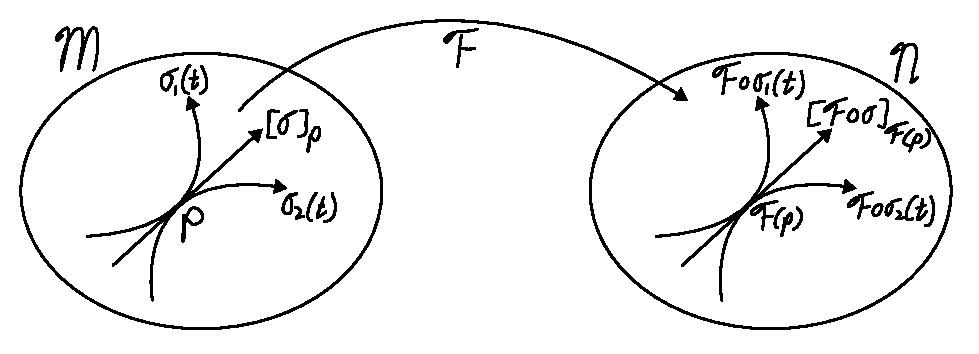
\includegraphics[width=0.7\textwidth, trim={0cm 0cm 0cm 0cm},clip]{push forward map}
      \caption[]{The push forward of an equivalence class of curves
      $[\sigma]_p$ induced by the map $\mathcal{F}$.}
      \label{fig: push forward map}
    \end{figure}
    \subsection{Calculating a push-forward of a tangent vector}
      \label{subsec: calculating a push-forward of a tangent vector}
      From definition~\ref{defn: push-forward defn}, we have
      \[\mathcal{F}_{*}(V_p^\sigma) = [\mathcal{F} \circ
      \sigma]_{\mathcal{F}(p)} = W^{\sigma^\prime}_{\mathcal{F}(p)}\]
      where $W^{\sigma^\prime}_{\mathcal{F}(p)} \in
      T_{\mathcal{F}(p)}(\mathcal{M})$. Now, for all $f \in
      C^k(\mathcal{N})$,
      \begin{align}
        W^{\sigma^\prime}_{\mathcal{F}(p)}(f) &=
        \left[\mathcal{F}_{*}(V_p^\sigma)\right](f) \nonumber \\
        &=\frac{d}{dt}\big[\mspace{-10mu}\underbrace{f \circ
        \mathcal{F}}_{\substack{\equiv f^\prime, \\
          f^\prime\in C^k(\mathcal{M})}} \mspace{-9mu} \circ\,
        \sigma\big](t)\Bigr|_{t = 0} \nonumber \\
        &= \frac{d}{dt}\big[f^\prime \circ \sigma \big](t)\Bigr|_{t = 0}\nonumber \\
        &= V^\sigma_p(f^\prime) \nonumber \\
        &= V^\sigma_p(f \circ \mathcal{F}) \label{eqn: important push forward result}
      \end{align}
    Now, in local charts $(U,\phi)$ and $(V,\psi)$ for $\mathcal{M}$ and
    $\mathcal{N}$ respectively, where for $p \in \mathcal{M}$ we define
    $\phi(p) \equiv x$ and $\psi(\mathcal{F}(p)) \equiv y$,
    equation~\ref{eqn: important push forward result} just reduces to:
    \begin{gather}
      % \label{eqn: push forward local chart}
      \left( W^{\sigma^\prime}_{\mathcal{F}(p)} \right)^i
      \left(\frac{\bar{f}(\mathcal{F}(p))}{\partial y^i}\right) =
      \left(V_p^\sigma\right)^i\left(\frac{\bar{f}(\mathcal{F}(p))}{\partial
      x^i}\right) \label{eqn: push forward local chart part 1} \\
      \implies \left( W^{\sigma^\prime}_{\mathcal{F}(p)} \right)^i
      \left(\frac{\partial \bar{f}(y^1,...,y^m)}{\partial y^i}\right) =
      \left(V_p^\sigma\right)^i\left(\frac{\partial \bar{f}(y^1(x^1,...,x^m),...,y^m(x^1,...,x^m))}{\partial
      x^i}\right)
    \end{gather}
    where $\bar{f} = f \circ \psi^{-1}$. This finally gives us:
    \begin{equation}
      \label{eqn: push forward local chart part 3}
      \left( W^{\sigma^\prime}_{\mathcal{F}(p)} \right)^i
      \left(\frac{\partial \bar{f}(y^1,...,y^m)}{\partial y^i}\right) =
      \left(V_p^\sigma\right)^i \frac{\partial y^j}{\partial x^i}
      \left(\frac{\partial \bar{f}(y^1,...,y^m)}{\partial y^j}\right)
    \end{equation}
    The detailed working to fully derive equation~\ref{eqn: push forward
    local chart part 3} is done in the context of fields in
    corollary~\ref{corollary: f-related field calculation}, but the working
    in corollary~\ref{corollary: f-related field calculation} can be easily
    adapted to quickly properly derive equation~\ref{eqn: push forward
    local chart part 3}.

    The hope is that the reader can see equation~\ref{eqn: push forward
    local chart part 1} as intuitive from equation~\ref{eqn: important push
    forward result} (if not, stare at it until it becomes intuitive).
    
    We will use the calculation here when we talk about
    $\mathcal{F}$-related vector fields in section~\ref{sec: mapping
    of vector fields} to derive some cool results for vector fields.
  \subsection{Push forward map induced by a curve}
    \label{subsec: push forward induced by a curve}
    Recall that a curve $\sigma$ on a manifold is an injective map from $I
    \subset \mathbb{R} \rightarrow \mathcal{M}$. Now, we can treat $I
    \subset \mathbb{R}$ as an open set of the one-dimensional manifold
    $\mathbb{R}$. This manifold, which admits a global chart, has a one
    dimensional tangent space $T_s(\mathbb{R})$ for all $s \in \mathbb{R}$.
    We can characterise the basis vector of the tangent space as
    $\frac{d}{dt}\Bigr|_{t=s}$ (here the coordinates of the manifold are
    labelled by $t$).

    Then, a tangent vector on $\mathcal{M}$ at the point $p = \sigma(s)$
    can be defined as the push forward of the tangent vector $\frac{d}{dt}\Bigr|_{t=s}$ induced by $\sigma$. I.e,
    \begin{equation}
      \sigma_{*}\left(\frac{d}{dt}\right)_{t = s} = V_{\sigma(s)} \in
      T_{\sigma(s)}(\mathcal{M})
    \end{equation}
    We will see this again when we talk about integral curves in
    section~\ref{sec: integral curves}.
  \subsection{Push forward map induced by a homeomorphism to
  $\mathbb{R}^m$}
    \label{subsec: push forward map induced by a homeomorphism}
    At a point $p \in \mathcal{M}$, under a local chart $(U,\phi)$, we
    recall that $T_p(\mathcal{M})$ has a coordinate basis
    $\left\{\frac{\partial}{\partial x^i}\right\}_{i = 1,...,m}$. Then, the
    map $\phi^{-1}$ induces a push-forward map between the coordinate basis
    in the local chart, and the actual basis vectors of $T_p(\mathcal{M})$,
    which we denote as: $\left\{e_i\right\}_{i = 1,...,m}$.
    \chapter{Vector Fields and Integral Curves}
  \subsection*{A rough explanation of vector fields and integral curves}
    So far we have only dealt with $T_p(\mathcal{M})$, the vector space of
    all tangent vectors at a point $p \in \mathcal{M}$. In this section, we
    introduce another mathematical object known as a vector field $X$, which
    roughly speaking, assigns \textbf{one} tangent vector to each point $p$
    on a $C^\infty$ (i.e smooth) manifold $\mathcal{M}$ in a \textbf{smooth}
    manner\footnote{The meaning of smooth assignment will be explained more
    precisely later}. Different vector fields $X_1$, $X_2$ \dots etc are
    different assignments of tangent vectors to each point $p \in
    \mathcal{M}$.

    A familiar example would be the electric field in $\mathbb{R}^3$; to
    each point $p \in \mathbb{R}^3$, we have an electric field vector, which
    is an element of $T_p(\mathbb{R}^3)$ (which is a 3 dimensional real
    vector space). Different electric fields lead to different assignments of
    electric field vectors to all points in $\mathbb{R}^3$.

    Another way of thinking about vector fields would be to imagine a
    family of \textbf{non-intersecting} smooth curves that fill
    $\mathcal{M}$. Then, for each point on the manifold, we assign to it a
    vector that is tangent to the curve that is passing through that point.
    Such curves are known as integral curves.

    An example would be consider a magnetic field pointing straight up and
    changing with time. We know from undergraduate EM that the
    equipotential curves are just concentric circles, and the electric
    field at a point is tangent to the concentric circle passing through
    that point. The concentric circles are the integral curves, and the
    electric field is the vector field for those integral curves. 

    Now, let's see the precise meaning of all of the above.
  \subsection*{The precise definition of a vector field}
    \begin{definition}[Vector field]
      \label{defn: vector field}
      A vector field $X$ on a $C^\infty$ manifold is a smooth assignment of a
      tangent vector $X_p \in T_p(\mathcal{M})$ at each point
      $p\in\mathcal{M}$ where "smooth" is defined to mean that, for all $f\in
      C^\infty(\mathcal{M})$, the function \[Xf: \mathcal{M} \rightarrow \mathbb{R}\]
      defined by:
      \[p \rightarrow (Xf)(p) = X_p(f)\]
      is infinitely differentiable.
    \end{definition}
    \begin{remark}
      There is a lot to unpack in definition~\ref{defn: vector field}.
      Points~\ref{item: local chart vector field part 1}, \ref{item: local
      chart vector field part 2} are especially important, because
      definition~\ref{defn: vector field} will make a lot more sense once we
      go into a local chart.
      \begin{enumerate}
        \item{Notice how we wrote $X_p$ instead of $X^\sigma_p$. We don't
        write $\sigma$ here because in the past, $\sigma$ referenced an
        entire equivalence class of curves, where different $\sigma$ would
        give different tangent vectors at the point $p$, but now there is
        just \textbf{one} tangent vector at the point $p$, which is assigned
        by the vector field. If you really want to think about curves, then
        $X_p$ is the vector tangent to the integral curve at the point $p$.}
        \item{$X$ is a map from $C^\infty(\mathcal{M})$ to
          $C^\infty(\mathcal{M})$. Notice how $f \in C^\infty(\mathcal{M})$
          and $Xf \in C^\infty(\mathcal{M})$. To easily see why $Xf \in
          C^\infty(\mathcal{M})$,
          we can write $Xf = X_{(\,\,)}(f)$ such that:
          \begin{align*}
            Xf: \mathcal{M} \rightarrow& \mathbb{R}\\
            p \mapsto& X_{(p)}(f)
          \end{align*}}
        \item{\label{item: local chart vector field part 1}Consider a local chart
        $(U,\phi)$. Then, in this local chart, with $x = \phi(p) = (x^1,...,x^m)$, we have:
        \begin{equation}
          \label{eqn: local chart vector field}
          \begin{split}
          (Xf)(p) &= X_p(f) \\
          &= X^i(x) \frac{\partial}{\partial x^i}\Big(\bar{f}(x)\Big)\Bigr|_{x}
          \end{split}
        \end{equation}
        where $\bar{f} = f \circ \phi^{-1}$, and where we write $X^i(x)$ to
        remind ourselves that the components of $X_p$ in the local chart
        depend on $\phi(p) = x$, and we also write $\frac{\partial}{\partial
        x^i}\big(\bar{f}(x)\big)\Bigr|_{x}$ to show that this partial
        derivative is evaluated at the point $\phi(p) = x$.
        
        Thus, "smooth assignment of of a tangent vector $X_p \in
        T_p(\mathcal{M})$ at each point $p\in\mathcal{M}$" just means that
        the last line in equation~\ref{eqn: local chart vector field} is a
        smooth function of $x$ when we vary $x$. Varying $x$ simply means
        moving to another point $p$ on the manifold, because $x = \phi(p)$.
        In other words, we want \[X^i(x) \frac{\partial}{\partial
        x^i}\Big(\bar{f}(x)\Big)\Bigr|_{x}: \mathbb{R}^m \rightarrow
        \mathbb{R}\] to be an infinitely differentiable function of $x$.}
        \item{\label{item: local chart vector field part 2}Again, consider a
        local chart $(U, \phi)$, where $x = \phi(p)$. If we write
        \begin{equation*}
          (Xf)(p) = (Xf) \circ \phi^{-1} \circ \phi(p) \equiv \overline{Xf}(x)
        \end{equation*}
        we have, comparing with our work from point~\ref{item: local chart
        vector field part 1},
        \begin{equation*}
          \overline{Xf}(x) = X^i(x) \frac{\partial}{\partial
          x^i}\Big(\bar{f}(x)\Big)\Bigr|_{x}
        \end{equation*}
        Thus, we can write: 
        \begin{align*}
        \overline{X}: C^\infty(\mathbb{R}^m) &\rightarrow C^\infty(\mathbb{R}^m)\\
        \bar{f} &\mapsto \overline{Xf}  = X^i(\,\,) \frac{\partial}{\partial
        x^i}\Big(\bar{f}(\,\,)\Big)\Bigr|_{(\,\,)}
        \end{align*}
        where
        \begin{align*}
          \overline{Xf}:
          \mathbb{R}^m
          &\rightarrow \mathbb{R}\\
          x &\mapsto X^i(x) \frac{\partial}{\partial
          x^i}\Big(\bar{f}(x)\Big)\bigr|_{x}
        \end{align*}
        Thus, we see that the local representation of $X$ in a coordinate
        chart is \[\overline{X} = X^i(\,\,) \frac{\partial}{\partial x^i}\]
        I.e, just like how $X$ takes in a point $p \in \mathcal{M}$ and returns a tangent vector $X_p$ at the point $p \in \mathcal{M}$, 
        $\overline{X}$ takes in $x =\phi(p) \in \mathbb{R}^m$ and returns a
        tangent vector $X^i(x) \frac{\partial}{\partial x^i}$ at the point $x
        \in \mathbb{R}^m$, where $X^i(x) \frac{\partial}{\partial x^i}$ is a smooth function of $x$.}
      \end{enumerate}
    \end{remark}
  \subsection*{The vector space of all vector fields
    $\mathcal{X}(\mathcal{M})$}
    Let $\mathcal{X}(\mathcal{M})$ be the set of all vector fields on the
    manifold $\mathcal{M}$. For $X,Y \in \mathcal{X}(\mathcal{M})$ and
    $\alpha \in \mathbb{R}$, we define the addition operator between two vector fields and the scalar multiplication operation as:
    \begin{subequations}
      \label{eqn: vector space of all vector fields operations}
      \begin{gather}
        (X + Y)f = X(f) + Y(f) \\
        (\alpha X)(f) = \alpha (X(f))
      \end{gather}
    \end{subequations}
    $\forall f\in C^\infty(\mathcal{M})$. From definition~\ref{defn:
    vector field}, since the addition of two tangent vectors at a point
    give a third tangent vector at a point, it is clear that
    $\mathcal{X}(\mathcal{M})$ together with the operations defined in
    equations~\ref{eqn: vector space of all vector fields operations} has a
    vector space structure.

    Thus, we shall denote $\mathcal{X}(\mathcal{M})$ as the vector space of all vector fields on the manifold $\mathcal{M}$.

    It is also meaningful to define the multiplication of a function $f \in
    C^\infty(\mathcal{M})$ with a vector field $X \in
    \mathcal{X}(\mathcal{M})$. I.e:
    \begin{align*}
    f\cdot X: C^\infty(\mathcal{M}) \rightarrow& C^\infty(\mathcal{M}) \\
    g\mapsto&
    (f\cdot X)(g)\\
    &\equiv f\cdot X(g)
    \end{align*}
    where $f\cdot X(g) \in C^\infty(\mathcal{M})$ is a map from
    $\mathcal{M}$ to $\mathbb{R}$, i.e \[ \left(f\cdot X(g)\right)(p) =
    f(p)\cdot(Xg)(p)\]
  \subsection*{Vector fields as derivations}
    From definition~\ref{defn: vector field}, we see that the map $X: C^\infty(\mathcal{M}) \rightarrow C^\infty(\mathcal{M})$ has all the properties of a derivation, since each $X_p$ is a derivation. These properties are:
    \begin{subequations}
      \begin{gather}
      X(f+g) = X(f) + X(g) \\
      X(rf) = r X(f) \\
      X(f\cdot g) = f\cdot X(g) + g\cdot X(f) \label{eqn:vector field leibniz rule}
      \end{gather}
    \end{subequations}
    where $f,g \in C^\infty(\mathcal{M})$, $r \in \mathbb{R}$.
  \section{Lie algebra structure}
    Now, we ask ourselves: can two vector fields be multiplied together to
    give a third field? Since each $X \in \mathcal{X}(M)$ is a map from
    $C^\infty(\mathcal{M})$ to $C^\infty(\mathcal{M})$, it seems reasonable
    to define the multiplication of two fields $X,Y$ as $X \cdot Y \equiv X \circ Y$, where $\forall f \in C^\infty(\mathcal{M})$, we have:
    \begin{equation}
      \label{eqn: bad vector field multiplication part 1}
      X \circ Y(f) = X(Y(f))
    \end{equation}
    However, equation~\ref{eqn: bad vector field multiplication part 1} is
    a bad definition, because $X\circ Y$ is not a vector field; $X\circ Y$
    fails to satisfy one of the properties of derivations, namely
    equation~\ref{eqn:vector field leibniz rule}.
    I.e, if $X\circ Y$ were a vector field, we should expect:
    \begin{equation*}
      [X\circ Y] (f\cdot g) = f\cdot [X\circ Y](g) + g \cdot [X\circ Y](f)
    \end{equation*}
    But instead, we have:
    \begin{align}
      [X\circ Y] (f\cdot g) &= X(Y(f\cdot g)) \nonumber \\
      &= X(f\cdot Y(g) + g\cdot Y(f)) \nonumber \\
      &= X(f\cdot Y(g)) + X(g\cdot Y(f)) \nonumber \\
      &= f\cdot X(Y(g)) + Y(g)\cdot X(f) + g\cdot X(Y(f)) + X(g) \cdot Y(f)\nonumber  \\
      &= f\cdot [X\circ Y](g) + g \cdot [X\circ Y](f) + \Big\{Y(g)\cdot X(f) +
      X(g) \cdot Y(f) \Big\} \label{eqn: bad vector field multiplication part 2}
    \end{align}
    We see the two extra terms at the end $Y(g)\cdot X(f)$ and
    $X(g) \cdot Y(f)$ prevent $[X\circ Y]$ from being a vector field.

    However, we can easily get rid of the last two terms; if we repeat the
    same calculations we did to arrive at equation~\ref{eqn: bad vector
    field multiplication part 2}, but for $[Y\circ X]$, we would arrive at:
    \begin{equation}
      \label{eqn: bad vector field multiplication part 3}
      [Y\circ X] (f\cdot g) = f\cdot [Y\circ X](g) + g \cdot [Y\circ X](f) + \Big\{Y(g)\cdot X(f) +
      X(g) \cdot Y(f) \Big\}
    \end{equation}
    Then, subtracting equation~\ref{eqn: bad vector field multiplication
    part 3} from equation~\ref{eqn: bad vector field multiplication part
    2}, we obtain:
    \begin{equation}
      \label{eqn: good vector field multiplication}
      [X,Y](f.g) = f[X,Y](g) + g[X,Y](f)
    \end{equation}
    where we have defined 
    \begin{equation}
      \label{eqn: commutator defn}
      [X,Y] \equiv X\circ Y - Y \circ X
    \end{equation}
    $[X,Y]$ is known as the commutator of the two vector fields $X,Y$. It
    is also called the Lie Bracket, for reasons that will become more clear
    when we talk about the Lie Derivative.

    Thus, we see from equation~\ref{eqn: good vector field multiplication}
    that while $X \circ Y$ and $Y \circ X$ aren't vector fields because
    they don't satisfy equation~\ref{eqn:vector field leibniz rule}, the
    commutator $[X,Y]$ is a vector field because it does (we can also
    easily show that the commutator satisfies all the other properties of a
    derivation). Now, let's see what the commutator looks like in a local chart $(U,\phi)$.
    \subsection{The commutator $[X,Y]$ in a local chart $(U, \phi)$}
      Consider a local chart $(U, \phi)$. Then, $\forall f \in
      C^\infty(\mathcal{M})$, $\forall p \in M$, we can write
      \begin{align*}
        \Big([X,Y](f)\Big)(p) &= \Big([X,Y](f)\Big) \circ \phi^{-1} \circ
        \phi(p) \\
        &= \overline{[X,Y](f)}(x)
      \end{align*}
      where $x = \phi(p)$ and $\overline{[X,Y](f)} = \big([X,Y](f)\big)
      \circ \phi^{-1}$ Now, we have:
      \begin{align*}
        \overline{[X,Y](f)}(x) =& \overline{[X(Y(f)) - Y(X(f)]}(x) \\
        =& \overline{X(\mspace{-10mu}\underbrace{Y(f)}_{\bar{k}\in
          C^\infty(\mathbb{R}^m)}\mspace{-10mu})}(x) -
          \overline{Y(\mspace{-10mu}\underbrace{X(f)}_{\bar{h}\in
          C^\infty(\mathbb{R}^m)}\mspace{-10mu})}(x) \\
        =& \overline{X(k)}(x) - \overline{Y(h)}(x) \\
        =& X^i(x)\frac{\partial}{\partial x^i}(\bar{k}) -
        Y^i(x)\frac{\partial}{\partial x^i}(\bar{h}) \\
        =& X^i(x)\frac{\partial}{\partial x^i}\left( Y^j(x)
        \frac{\partial\bar{f}(x)}{\partial x^j}\right) -
        Y^i(x)\frac{\partial}{\partial x^i}\left( X^j(x)
        \frac{\partial\bar{f}(x)}{\partial x^j}\right) \\
        =& X^i(x)\left(\frac{\partial \bar{f}(x)}{\partial x^j}\frac{\partial
        Y^j(x)}{\partial x^i} + Y^j(x)\frac{\partial^2 \bar{f}(x)}{\partial x^i \partial
        x^j}\right) - \\
        &Y^i(x)\left(\frac{\partial \bar{f}(x)}{\partial
        x^j}\frac{\partial X^j(x)}{\partial x^i} + X^j(x)\frac{\partial^2
        \bar{f}(x)}{\partial x^i \partial x^j}\right) \\
        =& \left(X^i(x) \frac{\partial Y^j(x)}{\partial x^i}
        \frac{\partial}{\partial x^j} - Y^i(x) \frac{\partial
        X^j(x)}{\partial x^i} \frac{\partial}{\partial x^j}\right)\bar{f}(x)
      \end{align*}
      Thus, we see that $\overline{[X,Y]}$ can be written as:
      \begin{equation}
        \label{eqn: commutator in local chart}
        \left(X^i \frac{\partial}{\partial x^i}Y^j - Y^i
        \frac{\partial}{\partial x^i}X^j\right) \frac{\partial}{\partial x^j}
      \end{equation}
    \subsection{Properties of the commutator $[X,Y]$}
      Clearly, from the definiton of the commutator in equation~\ref{eqn:
      commutator defn}, we have:
      \begin{subequations}
        \begin{gather}
          [X,Y] = -[Y,X] \\
          [X,[Y,Z]] + [Z,[X,Y]] + [Y,[Z,X]] = 0 \label{eqn: Jacobi identity}
        \end{gather}
      \end{subequations}
      where $X,Y,Z \in \mathcal{X}(\mathcal{M})$. By the way,
      equation~\ref{eqn: Jacobi identity} is known as the Jacobi
      identity.\footnote{Equation~\ref{eqn: Jacobi identity} is proved in
      the tutorials.}

      Now, the above two properties are essential elements in the structure
      of a Lie algebra. Formally, a Lie algebra is defined to be a real
      vector space $\mathcal{L}$ with a bilinear map $\mathcal{L} \times
      \mathcal{L} \rightarrow \mathcal{L}$ denoted by $(A,B) \mapsto [A,B]$
      which satisfies the following conditions:
      \begin{enumerate}
        \item{$\forall A,B \in \mathcal{L}$, \[[A,B] = - [B,A]\]}
        \item{$\forall A,B,C \in \mathcal{L}$, \[[A,[B,C]] +[C,[A,B]] +
        [B,[C,A]] = 0\]}
      \end{enumerate}
      We will come back to this when we discuss Lie groups and their associated tangent spaces.
  \section{Mapping of Vector Fields}
    \label{sec: mapping of vector fields}
    In section~\ref{sec: push forward between tangent spaces}, we
    saw how a differentiable map $\mathcal{F}: \mathcal{M} \rightarrow
    \mathcal{N}$ induces a map $\mathcal{F}_{*}:T_p(\mathcal{M})
    \rightarrow T_p(\mathcal{N})$ known as the push-forward map.
    \subsection*{Question: does $\mathcal{F}$ also induce a map from
    $\mathcal{X}(\mathcal{M})$ to $\mathcal{X}(\mathcal{N})$?}
      A natural way to define this induced map would be:
      \begin{equation}
        \label{eqn: attempt at defining induced map}
        \left(\mathcal{F}_{*}X\right)_{\mathcal{F}(p)} =
        \mathcal{F}_{*}(X_p)
      \end{equation}
      I.e, we define a vector field $Y = \mathcal{F}_{*}X$ in $\mathcal{N}$
      such that at the point $\mathcal{F}(p) \in \mathcal{N}$, there is a
      vector $\mathcal{F}_{*}(X_p) \in T_{\mathcal{F}(p)}(\mathcal{N})$.
      Now, equation~\ref{eqn: attempt at defining induced map} if a good attempt at defining this induced map, but it fails for two reasons:
      \begin{enumerate}
        \item{If $\mathcal{F}$ is not injective, then there might be two
        different points, $p_1,p_2 \in \mathcal{M}$ that map to the same
        point in $\mathcal{N}$, i.e $\mathcal{F}(p_1) = \mathcal{F}(p_2)$.
        In this case, should the induced vector at $\mathcal{F}(p_1) =
        \mathcal{F}(p_2)$ be $\mathcal{F}_{*}(X_{p_1})$, or
        $\mathcal{F}_{*}(X_{p_2})$?}
        \item{If $\mathcal{F}$ is not surjective, then $\exists p \in
        \mathcal{N}$ that don't have a pre-image in $\mathcal{M}$. How then
        should we assign a vector to $p\in \mathcal{N}$?}
      \end{enumerate}
      \begin{figure}
        \centering
        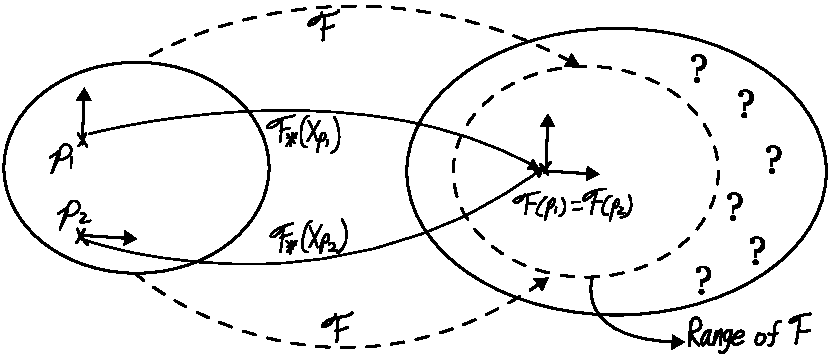
\includegraphics[width=0.7\textwidth, trim={0cm 0cm 0cm 0cm},clip]{push forward fail}
        \caption[]{}
        \label{fig: push forward fail}
      \end{figure}
      These two reasons are summarised in Figure~\ref{fig: push forward
      fail}. In summary, if $\mathcal{F}$ is not bijective (i.e if
      $\mathcal{F}$ is not a diffeomorphism), then $\mathcal{F}$ does not
      induce a map between $\mathcal{X}(\mathcal{M})$ and
      $\mathcal{X}(\mathcal{N})$.

      However, if $\mathcal{F}$ is a diffeomorphism, then the definition in
      equation~\ref{eqn: attempt at defining induced map} would be good,
      and $\mathcal{F}$ does indeed induce a map between
      $\mathcal{X}(\mathcal{M})$ and $\mathcal{X}(\mathcal{N})$. Let's put this in precise terms.
      
    \subsection{$\mathcal{F}$ related fields}
      \begin{definition}[$\mathcal{F}$ related fields\footnote{This
      definition is different from Kuldip's and is orignal...there might
      be some bugs.}]
        Let $\mathcal{F}: \mathcal{M} \rightarrow \mathcal{N}$ be a
        diffeomorphism, and let $X \in \mathcal{X}(\mathcal{M})$. Then,
        the diffeomorphism $\mathcal{F}$ induces a $\mathcal{F}$- related
        field $Y \in \mathcal{X}(\mathcal{N})$ by the following
        prescription:
        \[Y_{\mathcal{F}(p)} = \mathcal{F}_{*}(X_p)\]
        $\forall p \in \mathcal{M}$.

        We can write, $Y = \mathcal{F}_{*}\left(X\right)$ for the two
        $\mathcal{F}$-related vector fields $X,Y$.
      \end{definition}
      \remark{Informally, we shall say that the vector field $Y$ is the
      push-forward of the vector field $X$.}
      % , though strictly speaking this
      % is loose language (the push forward map is defined between tangent
      % spaces, but here we are only pushing forward one vector in the
      % tangent space of $p$ to give us another vector in the tangent space
      % of $\mathcal{F}(p)$).}
    \subsection{Some properties of $\mathcal{F}$ related fields}
      \begin{theorem}
        \label{theorem: f-related field calculation}
        Let $\mathcal{F}: \mathcal{M} \rightarrow \mathcal{N}$ be a
        diffeomorphism. If $X\in \mathcal{X}(\mathcal{M})$ and $Y\in
        \mathcal{X}(\mathcal{N})$ are $\mathcal{F}$-related, then
        $\forall f\in C^\infty(\mathcal{N})$, \[X\left(f \circ
        \mathcal{F}\right) = Y(f) \circ \mathcal{F}\]
      \end{theorem}
      \begin{remark}
        Given $p \in \mathcal{M}$, we can write theorem~\ref{theorem: f-related field calculation} in the following form:
        \[[X\left( f\circ \mathcal{F} \right)](p)= [Y(f)]\left(\mathcal{F}(p)\right)\]
        Remember that $f\circ \mathcal{F} \in C^\infty(\mathcal{M})$,
        and thus $X$ maps $f\circ \mathcal{F}$ to another function in $C^\infty(\mathcal{M})$.
      \end{remark}
      \begin{remark}
        Theorem~\ref{theorem: f-related field calculation} is very
        important. Given $X \in \mathcal{M}$, we can use
        theorem~\ref{theorem: f-related field calculation} to actually
        calculate $Y$. I.e, we can express the components of $Y$ in
        some local chart $(V,\psi)$ of $\mathcal{N}$ in terms of the
        components of $X$ in some local chart $(U,\phi)$ of
        $\mathcal{M}$. We will see how this works in
        corollary~\ref{corollary: f-related field calculation}.
      \end{remark}
      \begin{remark}
        Theorem~\ref{theorem: f-related field calculation} is the most important and the most powerful result of this section. All the other theorems in this section can be very easily proved by using this theorem.
      \end{remark}
      \begin{proof}[Proof of Theorem~\ref{theorem: f-related field
      calculation}]
        We begin by restating equation~\ref{eqn: important push forward
        result} which was derived in subsection~\ref{subsec:
        calculating a push-forward of a tangent vector}. For a
        diffeomorphism $\mathcal{F}:\mathcal{M} \rightarrow
        \mathcal{N}$, we have, $\forall f \in C^\infty(\mathcal{N})$,
        \begin{align*}
          W^{\sigma^\prime}_{\mathcal{F}(p)}(f) &\equiv
          [\mathcal{F}_{*}\left(V^\sigma_p\right)](f) \\
          &= V^\sigma_p(f \circ \mathcal{F})
        \end{align*}
        where $W^{\sigma^\prime}_{\mathcal{F}(p)} \in
        T_{\mathcal{F}(p)}(\mathcal{N})$, $\sigma^\prime = \sigma \circ
        \mathcal{F}$. Applying this result to the the
        $\mathcal{F}$-related fields $Y$ and $X$, we have, $\forall p
        \in \mathcal{M}$ and $\forall f \in C^\infty(\mathcal{N})$,
        \begin{align*}
          Y_{\mathcal{F}(p)}(f) &= \mathcal{F}_{*}(X_p)(f) \\
          \implies Y_{\mathcal{F}(p)}(f) &= X_p(f \circ \mathcal{F}) \\
          \implies [Y(f)](\mathcal{F}(p)) &= [X(f\circ \mathcal{F})](p) \\
          \implies [Y(f) \circ \mathcal{F}](p) &= [X(f\circ \mathcal{F})](p)
        \end{align*}
        which immediately gives us the desired result.
      \end{proof}
      \begin{corollary}[Theorem~\ref{theorem: f-related field calculation}, but in local coordinates.]
        \label{corollary: f-related field calculation}
        \mbox{} \\
        Let $(U,\phi)$ be a local chart in $\mathcal{M}$ and $(V,
        \psi)$ be a local chart in $\mathcal{N}$. Then,
        $\overline{\mathcal{F}} = \psi\circ\mathcal{F}\circ \phi^{-1}$
        is a map from $\phi(U) \subset \mathbb{R}^M$ to $\psi(V)
        \subset \mathbb{R}^M$. The situation is depicted in
        figure~\ref{fig: differentiable map defn}. For $p \in
        \mathcal{M}$, let $\phi(p) = (x^1,...,x^m)\equiv x$, and
        $\psi\left(\mathcal{F}(p)\right) = \overline{\mathcal{F}}(x) =
        (y^1,...,y^m) \equiv y$.
        Then, we have:
        \begin{align}
          [X\big( \mspace{-10mu} \underbrace{f \circ \mathcal{F}}_{\substack{\equiv
          f^\prime,  \\ f^\prime\in C^k(\mathcal{M})}}
          \mspace{-10mu}\big)](p) &=
          [Y(f)]\left(\mathcal{F}(p)\right) \nonumber \\
          \implies [X(f^\prime)]\circ \phi^{-1} \circ \phi(p) &=
          [Y(f)]\circ \psi^{-1} \circ \psi \circ
          \mathcal{F}\circ\phi^{-1}\circ\phi(p) \nonumber \\
          \implies X^i(x)\frac{\partial }{\partial
          x^i}\bar{f^\prime}(x)\biggr|_x &=
          Y^j(y)\frac{\partial}{\partial y^j} \bar{f}(y)\biggr|_y \nonumber
          % \label{eqn: local coord theorem 4.1}
        \end{align}
        where in the last line above, we used the fact that $\psi \circ
        \mathcal{F}\circ\phi^{-1}\circ\phi(p) =
        \overline{\mathcal{F}}(x) = y$. We also defined $\bar{f^\prime}
        \equiv f \circ \mathcal{F} \circ \phi^{-1}$, and $\bar{f}
        \equiv f \circ \psi^{-1}$. Now, we realise that:
        \begin{align*}
          \bar{f^\prime} &\equiv f \circ \mathcal{F} \circ \phi^{-1} \\
          &= f \circ \psi^{-1} \circ \psi \circ \mathcal{F} \circ
          \phi^{-1} \\
          &= \bar{f} \circ \overline{\mathcal{F}}
        \end{align*}
        which means that \[\bar{f^\prime}(x) = \bar{f}(y) =
        \bar{f}(y^1(x^1,...,x^m),..,y^m(x^1,...,x^m))\] where in the
        last equality, we realise that
        $\overline{\mathcal{F}}(x^1,...,x^m) = (y^1,...,y^m)$ defines
        $m$ coordinate transformation equations $\{y^i =
        y^i(x^1,...,x^m)\}_{i = 1,...,m}$

        Putting everything together, we have:
        \begin{align*}
          X^i(x) \left(\frac{\partial}{\partial x^i}
          \bar{f}(y^1(x^1,...,x^m),..,y^m(x^1,...,x^m))\right)\biggr|_x
          &= Y^j(y)\frac{\partial}{\partial y^j} \bar{f}(y)\biggr|_y \\
          \implies X^i(x) \frac{\partial y^j}{\partial x^i}\biggr|_x
          \frac{\partial}{\partial y^j} \bar{f}(y)\biggr|_y &=
          Y^j(y)\frac{\partial}{\partial y^j} \bar{f}(y)\biggr|_y
        \end{align*}
        which gives us:
        \begin{equation}
          \label{eqn: local representation of push forward map}
          Y^j(y) = X^i(x) \frac{\partial y^j}{\partial x^i}\biggr|_x
        \end{equation}
        Equation~\ref{eqn: local representation of push forward map} is
        super powerful. Given $X^i(x)$, which is the components of $X$
        in some local chart $(U,\phi)$ of $\mathcal{M}$, we are able to
        determine $Y^j(y)$, which are the components of the
        $\mathcal{F}$-related field in some local chart $(V,\psi)$ of
        $\mathcal{N}$. Note that here, $x = \phi(p)$, $y = \psi(p)$,
        and $y$ is related to $x$ via: $y = \psi \circ \mathcal{F}
        \circ \phi^{-1}(x) \equiv \overline{\mathcal{F}}(x)$.

        Note that \[\frac{\partial y^j}{\partial x^i}\biggr|_x\] are
        just elements of the Jacobian matrix of the $m$ coordinate
        transformation equations $\{y^i = y^i(x^1,...,x^m)\}_{i =
        1,...,m}$ induced by $y = \overline{\mathcal{F}}(x)$. Thus, if
        $\mathcal{M}$ and $\mathcal{N}$ are related by a diffeomorphism
        $\mathcal{F}$, then tangent vectors at $\mathcal{F}(p)\in
        \mathcal{N}$ are related to tangent vectors at $p\in
        \mathcal{M}$ via a linear transformation, where the linear
        transformation is given by the Jacobian matrix of the
        coordinate transformation equations. Pretty nifty result, eh.
      \end{corollary}
      \begin{theorem}
        \label{theorem: f related field other theorem}
        If $\mathcal{F}_{*}X_1 = Y_1$ and $\mathcal{F}_{*}X_2 = Y_2$,
        then $\forall f\in C^\infty(\mathcal{N})$ we have:
        \[\left([Y_1,Y_2](f)\right) \circ \mathcal{F} = [X_1, X_2](f
        \circ \mathcal{F})\]
      \end{theorem}
      \begin{proof}
        \begin{align*}
          \text{LHS} &= \left([Y_1,Y_2](f)\right) \circ \mathcal{F} \\
          &= \left(Y_1[Y_2(f)] - Y_1[Y_2(f)] \right) \circ \mathcal{F} \\
          &= Y_1[Y_2(f)] \circ \mathcal{F} - Y_2[Y_1(f)] \circ
          \mathcal{F} \\
          &= X_1[Y_2(f) \circ \mathcal{F}] - X_2[Y_1(f) \circ \mathcal{F}] \\
          &= X_1[X_2(f \circ \mathcal{F})] - X_2[X_1(f \circ \mathcal{F})]\\
          &= [X_1, X_2] (f\circ \mathcal{F}) \\
          &= \text{RHS}
        \end{align*}
      \end{proof}
      \begin{theorem}
        \[\mathcal{F}_{*}[X_1,X_2] =[\mathcal{F}_{*}
        X_1,\mathcal{F}_{*} X_2] \]
      \end{theorem}
      \begin{proof}
        Let $\mathcal{F}_{*}[X_1,X_2] = K$, where $K$ is to be determined.
        Then, $K$ and $[X_1,X_2]$ are $\mathcal{F}$-related fields. Thus,
        $\forall f \in C^\infty(\mathcal{N})$,
        \begin{align*}
          K(f) \circ \mathcal{F} 
          &= [X_1,X_2](f\circ \mathcal{F}) \\
          &= \left([\mathcal{F}_{*}X_1,\mathcal{F}_{*}X_1](f)\right) \circ
          \mathcal{F}
        \end{align*}
        Note that to get the last line, we used theorem~\ref{theorem: f
        related field other theorem}. Thus, we have $K =
        [\mathcal{F}_{*}X_1,\mathcal{F}_{*}X_1]$.
      \end{proof}
  \section{Integral Curves}
    \label{sec: integral curves}
    \begin{definition}[Integral Curve]
      \label{defn: integral curve defn}
      Let $V$ be a vector field on a manifold $\mathcal{M}$ and let $p$ be a point on $\mathcal{M}$. Then an integral curve of $V$ passing through the point $p$ is a curve $t \mapsto \gamma_p(t)$ such that
      \begin{subequations}
        \begin{gather}
          \gamma_p(0) = p \\
          {\gamma_{p}}_{*} \left(\frac{d}{dt}\right)\biggr|_{t = s} =
          V_{\gamma_p(s)} \label{eqn: integral curve push forward eqn}
        \end{gather}
      \end{subequations}
      for all $s$ in some open interval $I = (-\epsilon, \epsilon)$ of $\mathbb{R}$.
    \end{definition}
    \begin{remark}
      Recall that a curve is an injective map from $\mathbb{R}$ to
      $\mathcal{M}$. Essentially, what this definition is saying is that for
      $\gamma_p(t)$ to be an integral curve of the vector field $V$, the
      push-forward map induced\footnote{See subsection~\ref{subsec:
      push forward induced by a curve} to see why a curve induces this
      push-forward map.} by $\gamma_p(t)$ must push-forward the basis
      vector of $T_s(\mathbb{R})$ to the vector assigned by the vector
      field at the point $\sigma(s) \in \mathcal{M}$. The other condition,
      $\gamma_p(0) = 0$ is just to make sure that the curve passes through
      $p \in \mathcal{M}$.
    \end{remark}
    \subsection{Local representation of an integral curve}
      Let's see what definition~\ref{sec: integral curves} means in a
      local coordinate chart $(U,\phi)$. For all $f \in
      C^\infty(\mathcal{M})$, we shall evaluate the LHS and the RHS of
      equation~\ref{eqn: integral curve push forward eqn}. The LHS is:
      \begin{align*}
        \text{LHS} &= \left({\gamma_{p}}_{*} \left(\frac{d}{dt}\right)\biggr|_{t =
        s}\right)(f) \\
        &= \frac{d}{dt} \Big(f\circ \gamma_p(t)\Big)\Bigr|_{t = s} \\
        &= \frac{d}{dt} \Big(f\circ \phi^{-1} \circ \phi \circ
        \gamma_p(t)\Big)\Bigr|_{t = s} \\
        &= \frac{d}{dt} \Big(\bar{f}[\phi(\gamma_p(t))]\Big)\Bigr|_{t = s} \\
        &= \frac{d}{dt}
        \Big(\bar{f}(x_p^1(t),x_p^2(t),...,x_p^m(t))\Big)\Bigr|_{t = s} \\
        &= \frac{\partial \bar{f}(x_p^1,...,x_p^m)}{\partial
        x_p^i}\Bigr|_{\phi(\gamma_p(s))} \frac{d x_p^i(t)}{dt}\Bigr|_{t =
        s}
      \end{align*}
      where the subscript $p$ reminds us that
      $(x_p^1(t),x_p^2(t),...,x_p^m(t))$ is a local representation of the
      integral curve passing through $p$. Note that this calculation,
      though it looks long, is nothing more than finding the tangent vector
      to the curve $\gamma(t)$ at point $p$ in a local chart $(U, \phi)$.
      
      Now, the RHS is:
    \begin{align*}
      \text{RHS} &= V_{\gamma_p(s)}(f) \\ 
      &= [V(f)](\gamma_p(s)) \\
      &= [V(f)]\circ \phi^{-1} \circ \phi \circ (\gamma_p(s)) \\
      &= [\overline{V(f)}](\overline{\gamma_p}(s))\\
      &= V^i(x_p^1(s),...,x_p^m(s)) \frac{\partial
      \bar{f}(x_p^1,...,x_p^m)}{\partial
      x_p^i}\biggr|_{\phi(\gamma_p(s))}
    \end{align*}
    where $\overline{\gamma_p}(s) = (x^1(s), x^2(s),...,x^m(s))$. Comparing
    the LHS and the RHS, we have:
    \begin{align}
      &V^i(x_p^1(s),...,x_p^m(s)) = \frac{d x_p^i(t)}{dt}\Bigr|_{t = s}
      \nonumber \\
      \implies & V^i(x_p^1(s),...,x_p^m(s)) = \frac{d x_p^i(s)}{ds}
      \label{eqn: integral curve eqn}
    \end{align}
    for $i = 1,...m$. Equation~\ref{eqn: integral curve eqn} is a first
    order differential equation, with the initial condition at $s = 0$,
    $(x^1(0), x^2(0),...,x^m(0)) = \phi(p)$. This is the equation which we
    will use to calculate, in some coordinate chart, the integral curve to
    the vector field passing through the point $p \in \mathcal{M}$.

    The existence and uniqueness theorem of ordinary differential equations
    guarantees that there is a unique solution to equation~\ref{eqn: integral curve eqn}, at least locally in a coordinate chart. It may be the cases that the integral curves is defined only on a setset of $\mathbb{R}$, in which case we have to pay attention so that the parameter $s$ does not exceed the given interval.

    It is known that\footnote{Not proven in Kuldip's notes, though the
    proof probably exists somewhere.} if $\mathcal{M}$ is a compact
    manifold, the integral curves exist for all $s \in \mathbb{R}$. This
    motivates the important definition of a complete vector field:

    \begin{definition}[Complete vector field]
      \label{complete vector field}
      A vector field $V$ on a manifold $\mathcal{M}$ is complete if, at
      every point $p \in \mathcal{M}$, the integral curve that passes
      through $p$ can be extended to an integral curve for $V$ that is
      defined for all $s \in \mathbb{R}$.
    \end{definition}

    \chapter{Cotangent Spaces and One Forms}
  \section{Linear algebra recap: The dual of a vector space}
    \label{sec: LA recap, dual of vector space}
    This section is merely a recap of linear algebra. For more information,
    one can refer to textbooks on linear algebra...

    Consider two vector spaces $V$ and $W$, and the set of all linear
    transformations from $V$ to $W$, denoted as $\mathcal{L}(V,W)$. On this
    set $\mathcal{L}(V,W)$, we define the binary addition operation as:
    \[(T_1 + T_2)(\vec{v}) = T_1(\vec{v}) + T_2(\vec{v})\]
    where $T_1,T_2 \in \mathcal{L}(V,W)$ and $\vec{v} \in V$.
    We also define the scalar multiplication operation as: 
    \[(cT)(\vec{v}) = cT(\vec{v})\] 
    where $T \in \mathcal{L}(V,W)$, $\vec{v} \in V$ and $c \in \mathbb{F}$
    where $\mathbb{F}$ is any field (e.g $\mathbb{R}$, $\mathbb{C}$).
    \begin{theorem}[$\mathcal{L}(V,W)$ with the binary addition and scalar
    multiplication defined above is a vector space over $\mathbb{F}$]
      \label{thm: lame dual space theorem}
    \end{theorem}
    \begin{proof}
      Left as an exercise, just verify that all the axioms of vector spaces
      are fulfilled. Note that the zero vector in $\mathcal{L}(V,W)$ is the
      zero map from $V$ to $W$, and the additive inverse of $T \in
      \mathcal{L}(V,W)$ is $-T \in \mathcal{L}(V,W)$, defined by $(-T)(\vec{v})
      = - T(\vec{v})$ where $\vec{v} \in V$.
    \end{proof}
    For the rest of this section, we shall assume that the field $\mathbb{F}$
    is $\mathbb{R}$. Now, we define the dual space of $V$ as $V^{*} \equiv
    \mathcal{L}(V, \mathbb{R})$\footnote{$\mathbb{R}$ has a vector space
    structure, so we can do this.}. From theorem~\ref{thm: lame dual space
    theorem}, $V^{*}$ has a vector space structure. We say that $V^{*}$ is
    the set of all linear functionals from $V$ to $\mathbb{R}$, i.e elements
    of $ V^{*} $ map $\vec{v} \in V$ to $\mathbb{R}$. 

    Suppose that $V$ has a basis $B = \{e_1, e_2, ... e_n\}$. Then, $V^*$ has
    a basis $B^* = \{f_1, f_2, ... f_n\}$ defined by: \[f_i(e_j) =
    \delta_{ij}\]
    
    Note that we can also write $V = \mathcal{L}(V^*, \mathbb{R})$, i.e we
    can consider $V$ the elements of $V$ as linear maps from $V^*$ to
    $\mathbb{R}$. In this case, we can write: \[e_i(f_j) = \delta_{ij}\]
    where $B = \{e_1, e_2, ... e_n\}$ is a basis of $V$ and $B^* = \{f_1,
    f_2, ... f_n\}$ is a basis of $V^*$. 

    To put both views on equal footing, we shall sometimes write: \[\langle
    v, k \rangle \equiv v(k) = k(v)\] where $v \in V$ and $k \in V^*$.
  \section{Cotangent Spaces}
    \label{sec: Cotangent Spaces}
    Now, we recall that $T_p(\mathcal{M})$ has a vector space structure.
    Thus, from section~\ref{sec: LA recap, dual of vector space}, we can
    define the another vector space dual to $T_p(\mathcal{M})$, which we
    shall denote as the cotangent space $T^*_p(\mathcal{M})$. Let's formalise this idea.
    \begin{definition}[Cotangent Space]
      The cotangent space at $p \in \mathcal{M}$ is defined as
      $T^*_p(\mathcal{M}) \equiv \mathcal{L}(T_p(\mathcal{M}), \mathbb{R})$.
    \end{definition}
    \begin{remark}
      I.e, $k \in T_p^*(\mathcal{M})$ is a real linear map from
      $T_p(\mathcal{M})$ into $\mathbb{R}$, defined by:
      \begin{align*}
        k: T_p(\mathcal{M}) &\rightarrow \mathbb{R} \\
        v &\mapsto \langle k, v \rangle_p
      \end{align*}
      where $v$ is any vector in $T_p(\mathcal{M})$, and the subscript $p$
      reminds us that all this happens only at a specific point $p \in
      \mathcal{M}$. 
    \end{remark}
    As per discussed in section~\ref{sec: LA recap, dual of vector space}, if
    $T_p(\mathcal{M})$ has a basis $\{e_1,...,e_m\}$, then the dual basis for
    $T^*_p(\mathcal{M})$, which we denote as $\{f^1,...,f^m\}$ can be
    uniquely determined by requiring that:
    \begin{equation}
      \label{eqn: dual basis defn}
      \langle f^i, e_j \rangle_p = \delta^i_j
    \end{equation}
    for all $i,j = 1,...,m$.
    \subsection{Note: positioning of indices}
      As the astute reader might have noticed, components of tangent vectors
      are labelled with upper indices, whereas basis vectors are labelled with
      lower indices. Similarly, components of cotangent vectors will be
      labelled with lower indices, and basis cotangent vectors will be labelled
      with upper indices. The position of the indices remind us of the
      transformation rules under a change of basis (i.e, when we move from one
      local chart to another). Things with upper indices transform
      contravariantly, like: \[v^{\prime i} = \frac{\partial x^{\prime
      i}}{\partial x^j} v^j\] whereas things with lower indices transform
      covariantly, like: \[k^{\prime}_i = \frac{\partial x^{j}}{\partial
      x^{\prime}_i} k_j \] It has been shown in the derivation of
      equation~\ref{eqn: Tangent vector component contravariant transformation}
      that the components of a tangent vector do indeed transform
      contravariantly, and it will be shown in subsection~\ref{subsec:
      transformation property of cotangent vectors under coord change} that
      components of a cotangent vector transform covariantly.
    \subsection{$T^*_p(\mathcal{M})$ in a local chart $(U, \phi)$}
      Recall that geometrically, tangent vectors are constructed from curves
      on a manifold. In a local chart $(U,\phi)$, a tangent vector
      $V^\sigma_p$ can be written as:
      \[V^\sigma_p \xrightarrow[\text{chart}]{\text{Local}} V^i
      \frac{\partial}{\partial x^i}\]
      Two important concepts to recall:
      \begin{enumerate}
        \item{$\{\frac{\partial}{\partial x^1},...,\frac{\partial}{\partial
          x^m}\}$ form a basis for $T_p(\mathcal{M})$ in a local chart. We
          can regard $\frac{\partial}{\partial x^i}$ as a directional
          derivative in the direction of increasing $x^i$.}
        \item{$V^\sigma_p$ in a local chart is just a linear combination of
          $\frac{\partial}{\partial x^i}$, where the components $V^i$ serve to
          produce a new directional derivative in the direction specified by
          $[\sigma]_p$.}
      \end{enumerate}
      Now, in a local chart, we want the dual basis of $T^*_p(\mathcal{M})$
      to be dual to $\{\frac{\partial}{\partial
      x^1},...,\frac{\partial}{\partial x^m}\}$, i.e we want to find a basis
      of $T^*_p(\mathcal{M})$ such that equation~\ref{eqn: dual basis defn}
      holds. Since in a local chart the $i$-th basis vector of
      $T_p(\mathcal{M})$ is a directional derivative in the direction of
      increasing $x^i$, a natural way to define the dual basis of
      $T^*_p(\mathcal{M})$ would be to define it as $\{dx^1,...,dx^m\}$, i.e
      we define the the $j$-th element of the dual basis to be a small change
      in the $x^j$ direction. The result is that we have: \[\left\langle
      \frac{\partial}{\partial x^i}, dx^j \right\rangle_{\phi(p)} =
      \frac{\partial}{\partial x^i}(dx^j) = \delta^j_i\] which automatically
      fulfils equation~\ref{eqn: dual basis defn}.
      
      Thus, for an arbitrary tangent vector $V^i \frac{\partial}{\partial
      x^i}$, we have:
      \[\left\langle V^i \frac{\partial}{\partial x^i}, dx^j
      \right\rangle_{\phi(p)} = V^j \]
      I.e, the basis cotangent vector $dx^j$ acting on an arbitrary tangent
      vector $V^i \frac{\partial}{\partial x^i}$ gives the length of that tangent
      vector in the $x^j$ direction.

      Anyway, since in a local chart $\{dx^1,...,dx^m\}$ is a basis for
      $T^*_p(\mathcal{M})$, we see that for $k \in T^*_p(\mathcal{M})$, $k$
      has local representation $k_i dx^i$.
  \section{The pull-back map between cotangent spaces}
    Recall from section~\ref{sec: push forward between tangent spaces} that
    under a mapping $\mathcal{F}: \mathcal{M} \rightarrow \mathcal{N}$ from a
    manifold $\mathcal{M}$ into a manifold $\mathcal{N}$, we could define the
    notion of a push-forward map between the tangent spaces of the two
    manifolds
    \[\mathcal{F}_* : T_p(\mathcal{M}) \rightarrow
    T_{\mathcal{F}(p)}(\mathcal{N})\]
    In the sense of cotangent spaces the map $\mathcal{F}$ induces a "pull-back" map between the two cotangent spaces:
    \[\mathcal{F}^* : T^*_{\mathcal{F}(p)}(\mathcal{N}) \rightarrow
    T^*_p(\mathcal{M})\]
    defined through
    \[\left\langle \mathcal{F}^*k, v \right\rangle_p = \left\langle
    k, \mathcal{F}_*v \right\rangle_{\mathcal{F}(p)}\] for all $k \in
    T^*_{\mathcal{F}(p)}(N)$ and $v \in T_p(\mathcal{M})$. Now, at this
    juncture we shall introduce a theorem regarding this pull-back map.
    \begin{theorem}[Composition of pull-back maps]
      Suppose that $\mathcal{M}$,$\mathcal{N}$,$\mathcal{P}$ are three differentiable manifolds with differentiable maps:
      \[\mathcal{M} \xrightarrow{\mathcal{F}_1} \mathcal{N}
      \xrightarrow{\mathcal{F}_2} \mathcal{P}\]
      Then, we have:
      \[\left(\mathcal{F}_2 \circ \mathcal{F}_1\right)^* = \mathcal{F}_1^*
      \circ \mathcal{F}_2^*\]
    \end{theorem}
    \begin{proof}[Rough sketch of a proof]
      First, we can easily prove that $\left( \mathcal{F}_2 \circ
      \mathcal{F}_1\right)_*$ = ${\mathcal{F}_2}_* \circ {\mathcal{F}_1}_*$.
      Then, we just use the definition of the pull-back map twice.
    \end{proof}

    The pull-back map defined above is very useful, and allows us to determine many properties of cotangent vectors based on the properties of tangent vectors. We shall see two applications below.

    \subsection{Application one: Constructing the basis for
    $T^*_p(\mathcal{M})$}
      Recall from subsection~\ref{subsec: push forward map induced by a homeomorphism} that if $\{\frac{\partial}{\partial
      x^1},...,\frac{\partial}{\partial x^1}\}$ is a basis of
      $T_p(\mathcal{M})$ in a local chart $(U, \phi)$, then the push forward
      map $\phi^{-1}_*$ allows us to determine the basis $\{e_1,...,e_m\}$ of
      $T_p(\mathcal{M})$.
      We can construct the basis for $T^*_p(\mathcal{M})$ in a similar way. We have: 
      \begin{align*}
        \left\langle \phi^* dx^i, e_j \right\rangle_p 
        &= \left\langle dx^i, \phi_*e_j \right\rangle_{\phi(p)} \\
        &= \left\langle dx^i, \frac{\partial}{\partial x^j} \right\rangle_{\phi(p)} \\
        &= \delta^i_j
      \end{align*}
      which tells if we define $f^i = \phi^* dx^i$, then $\{f^1,...,f^m\}$
      forms the dual basis for $T^{*}_p(\mathcal{M})$.
    \subsection{Application two: Transformation property of cotangent vectors under a change of coords}
      \label{subsec: transformation property of cotangent vectors under coord change}
      Suppose that $(U,\phi)$ and $(V,\psi)$ are two charts of a manifold
      $\mathcal{M}$. Consider a point $p \in U \cap V$. Let $k \in
      T^*_p(\mathcal{M})$ and $v \in T_p(\mathcal{M})$. Also, let $\bar{k},
      \bar{v}$ and $\bar{k}^\prime, \bar{v}^\prime$ be the coordinate
      representations of $k, v$ in the local charts $(U,\phi)$, $(V,\psi)$
      respectively. Aim: determine how the components of $\bar{k}^\prime$ are
      related to the components of $\bar{k}$.\\ Since we have:
      \begin{align*}
        \left\langle \bar{k}, \bar{v}\right\rangle_{\phi(p)}
        &= \left\langle \bar{k}, \phi_{*} v\right\rangle_{\phi(p)} \\
        &= \left\langle \phi^{*}\bar{k},  v\right\rangle_{p} \\
        &= \left\langle k,  v\right\rangle_{p}
      \end{align*}
      and we can similarly show:
        \[\left\langle \bar{k}^\prime, \bar{v}^\prime\right\rangle_{\psi(p)}
        = \left\langle k, v\right\rangle_{p}\]
      we arrive at this result:
        \begin{equation}
          \label{eqn: contraction coordinate independence}
          \left\langle \bar{k}^\prime, \bar{v}^\prime\right\rangle_{\psi(p)}
          = \left\langle \bar{k}, \bar{v}\right\rangle_{\phi(p)}
        \end{equation}
      First, we evaluate the LHS of equation~\ref{eqn: contraction coordinate
      independence} to give us:
      \begin{align}
        \left\langle \bar{k}^\prime, \bar{v}^\prime\right\rangle_{\psi(p)} 
        &= \bar{k}_{i}^{\prime} \bar{v}^{\prime j} \left\langle dx^{\prime i} ,
        \frac{\partial}{\partial x^{\prime j}} \right\rangle \nonumber \\
        &= \bar{k}_{i}^{\prime} \bar{v}^{\prime j} \delta^i_j \nonumber \\
        &= \bar{k}_{i}^{\prime} \bar{v}^{\prime i} \label{eqn:
        covector change of coord part 1}
      \end{align}
      Then, we can simiarly evaluate the RHS of equation~\ref{eqn: contraction coordinate independence} to give us:
      \begin{equation}
        \label{eqn: covector change of coord eqn part 2}
        \left\langle \bar{k}, \bar{v}\right\rangle_{\phi(p)} = \bar{k}_j
        \bar{v}^j
      \end{equation}
      Now, we know that $\overline{\mathcal{F}_*}\bar{v} = \bar{v}^\prime$,
      and we also know that $\bar{v}^{\prime i} = \frac{\partial x^{\prime
      i}}{\partial x^j} \bar{v}^j$. Thus, using this as well as
      equations~\ref{eqn: covector change of coord part 1}, \ref{eqn:
      covector change of coord eqn part 2} we have:
      \begin{gather}
        \left\langle \bar{k}^\prime, \bar{v}^\prime\right\rangle_{\psi(p)} =
        \left\langle \bar{k}, \bar{v}\right\rangle_{\phi(p)} \nonumber\\
        \implies \bar{k}_{i}^{\prime} \bar{v}^{\prime i} = \bar{k}_j
        \bar{v}^j \nonumber\\
        \implies \bar{k}_{i}^{\prime} \left(\frac{\partial x^{\prime
        i}}{\partial x^j} \bar{v}^j \right) = \bar{k}_j \bar{v}^j \nonumber\\
        \implies \bar{k}_{i}^{\prime} \left(\frac{\partial x^{\prime
        i}}{\partial x^j} \right) = \bar{k}_j \label{eqn: covector change of coord eqn part 3}
      \end{gather}
      We can then easily invert\footnote{We do this inversion either by
      swapping the primed and unprimed variables, or we write the equation in
      matrix form and then invert. When we do the latter approach, we realise
      that $\left(\frac{\partial x^j}{\partial x^{\prime i}} \right)$ is
      nothing more than just entries of the Jacobian matrix of the coordinate
      transform.} equation~\ref{eqn: covector change of coord eqn part 3} to
      give us:
      \begin{equation}
        \bar{k}_{i}^{\prime} = \left(\frac{\partial x^j}{\partial x^{\prime
        i}} \right) \bar{k}_j
      \end{equation}
      which tells us how the components of a cotangent vector transform under
      coordinate transformation. As can be seen, the components transform
      covariantly.
  \section{One-forms}
    \begin{definition}[1-form]
      \label{defn: one form defn}
      A one-form $\omega$ on $\mathcal{M}$ is a smooth assignment of a
      cotangent vector $\omega_p \in T_p^*(\mathcal{M})$ to each point $p \in
      \mathcal{M}$. Here, "smooth" means that for any vector field $X \in \mathcal{X}(\mathcal{M})$, the real-valued function
        \[ \left\langle\omega, \mathcal{X}\right\rangle(p) = \left\langle
        \omega_p, X_p \right\rangle\]
      is smooth.
    \end{definition}
    \begin{remark}
      To better understand the notion of smoothness, we first go to a local
      coordinate chart $(U, \phi)$. We note that:
      \begin{align*}
        \left\langle \omega_p, X_p \right\rangle_p
        &= \left\langle \phi^* \bar{\omega}_p, X_p \right\rangle_p \\
        &= \left\langle  \bar{\omega}_p, \phi_* X_p \right\rangle_{\phi(p)}\\
        &= \left\langle  \bar{\omega}_p, \bar{X}_p \right\rangle_{x}
      \end{align*}
      where in the last line, we have defined $x = \phi(p)$. Now, since
      $\bar{X}_p = \bar{X}^i(x) \frac{\partial}{\partial x^i}$ and
      $\bar{\omega}_p = \bar{\omega}_j(x) dx^j$, we have:
      \begin{equation}
        \label{eqn: one form smoothness defn part 1}
        \left\langle \omega_p, X_p \right\rangle_p = \bar{\omega}_i(x)
        \bar{X}^i(x)
      \end{equation}
      Thus, "smooth assignment of a cotangent vector $\omega_p$" in
      definition~\ref{defn: one form defn} just means that for any chart
      $(U,\phi)$ of $\mathcal{M}$, and for any $X \in
      \mathcal{X}(\mathcal{M})$, the expression $\bar{\omega}(x)_i
      \bar{X}^i(x)$ is a smooth function of $x$.

      In fact, since $X^i(x)$ is by definition already a smooth function of $x$, we just require $\omega_i(x)$ to be a smooth function of $x$.

      \paragraph{TL:DR} Let $(U, \phi)$ is an arbitrary chart of the
      manifold, and let $x = \phi(p)$ for arbitrary $p \in \mathcal{M}$. A
      one-form $\omega$ has a local coord representation of $\omega_i(x)
      dx^i$. The function $\omega_i(x)$ is a smooth function of $x$.
      \subsection{The pull-back of a one-form}
        The pull-back of a one-form is very similar to the pull-back of
        cotangent vector. Just note that since a one-form is a smooth
        assignment of cotangent vectors to all points in the manifold, we have to pull-back at every point in the manifold.
        \begin{definition}[Pull-back of a 1-form]
          Let $\mathcal{F}: \mathcal{M} \rightarrow \mathcal{N}$ be a
          differentiable map\footnote{I'm not sure if differentiable map is good enough...do we actually require a diffeomorphism? I'm not sure.} between two manifolds $\mathcal{M}$ and
          $\mathcal{N}$. If $\omega$ is a one-form on $\mathcal{N}$ then the
          pull-back of $\omega$ is the one-form $\mathcal{F}^*\omega$ on
          $\mathcal{M}$ defined by:
            \[\left\langle \mathcal{F}^*\omega, v \right\rangle_p =
            \left\langle \omega, \mathcal{F}_*v
            \right\rangle_{\mathcal{F}(p)} \]
          for all points $p \in \mathcal{M}$ and all tangent vectors $v \in T_p(\mathcal{M})$.
        \end{definition}
    \end{remark}

      
    \chapter{Tensors and Tensor fields}
  \section{Preliminaries: Linear Algebra recap}
    \label{sec: preliminaries linear algebra recap}
    \subsection{Multilinear maps}
      \label{subsec: multilinear maps}
      \begin{definition}[Multilinear maps]
        Let $V_1, V_2, ..., V_n; W$ be vector spaces. Let $V_1 \cross
        V_2,...,\cross V_n$ be set\footnote{This is just the Cartesian product
        btw.} of all ordered $n$-tuples $(v_1,v_2,...,v_n)$, where $v_i \in
        V_i$. A mapping \[\phi: V_1 \cross V_2 \cross ... \cross V_n
        \rightarrow W\] is called multilinear if it satisfies the condition
        \begin{equation*}
          \begin{split}
        \phi(v_1,v_2,...,(\alpha v_i + \beta v_i^\prime), v_{i+1}, ... ,&v_n) =
        \\
        \alpha \phi(v_1,v_2,...,v_i, v_{i+1}, ... ,&v_n) + \beta
        \phi(v_1,v_2,...,v_i^\prime, v_{i+1}, ... ,v_n)
          \end{split}
        \end{equation*}
        where $\alpha,\beta \in \mathbb{R}$, for $i = 1,2,...,n$.
      \end{definition}
      \begin{remark}
        Roughly speaking, a map $\phi$ is said to be multilinear if it is
        linear in each of its "variables" separately. We will denote the set of
        all multilinear maps of $V_1 \cross V_2,...,\cross V_n$ into $W$ as
        $\mathcal{L}(V_1,V_2,...,V_n;W)$. Then, the set $
        \mathcal{L}(V_1,V_2,...,V_n;W)$ becomes a vector space in a natural
        way. First, we define the binary addition operator as:
        \[\left(\phi_1 + \phi_2\right)(v_1,v_2,...,v_n) =\phi_1(v_1,v_2,...,v_n)
        + \phi_2(v_1,v_2,...,v_n)\]
        and the scalar multiplication operator as:
        \[\left(\alpha\phi\right)(v_1,v_2,...,v_n) =
        \alpha\phi(v_1,v_2,...,v_n)\]
        where $\phi_1,\phi_2,\phi \in \mathcal{L}(V_1,V_2,...,V_n;W)$ and
        $\alpha \in \mathbb{R}$.
        Then we can easily show that the set $\mathcal{L}(V_1,V_2,...,V_n;W)$
        with the binary addition and scalar multiplication operators fulfil the axioms of a vector space.

        It is important to note that the vector spaces $V_1,V_2,...,V_n$ can be
        either the tangent spaces $T_p(\mathcal{M})$ or the cotangent spaces
        $T^*_p(\mathcal{M})$, since both of these are vector spaces. The vector
        space $W$ which appears in $\mathcal{L}(V_1,V_2,...,V_n;W)$ can also be $\mathbb{R}$ (which also has a vector space structure).
      \end{remark}

    \subsection{Tensor product of vector spaces}
      Recall from section~\ref{sec: LA recap, dual of vector space} that if
      we have a vector space $V_1$, then $V^*_1 \equiv \mathcal{L}(V_1,
      \mathbb{R})$ is the set of all linear maps from $V_1$ to $\mathbb{R}$.
      We can also similarly write $V_1 = \mathcal{L}(V_1^*;\mathbb{R})$, i.e
      we can also regard $V_1$ as the set of all linear maps from $V_1^*$ to
      $\mathbb{R}$. We shall use this idea to define the concept of a tensor
      product of two vector spaces.

      \subsubsection{Illustration with two vector spaces $V_1$, $V_2$}
      Suppose that $V_1$ has a basis $\{e_1, e_2,...,e_n\}$ and $V_1^*$ has a
      corresponding dual basis $\{f_1,...,f_n\}$. Also, suppose we have
      another vector space $V_2 \equiv \mathcal{L}(V_2,\mathbb{R})$, with its
      corresponding dual $V_2^*$. Let the basis of $V_2$ be $\{e_1^\prime,
      e_2^\prime,...,e_n^\prime\}$, and let the basis of $V_2^*$ be
      $\{f_1^\prime, f_2^\prime,...,f_n^\prime\}$.\\
      Then, we define the tensor product of
      $V_1^*$ and $V_2^*$ as:
        \begin{equation}
          V_1^* \otimes V_2^* \equiv \mathcal{L}(V_1,V_2;\mathbb{R})
        \end{equation}
      From subsection~\ref{subsec: multilinear maps}, we see that $V_1^*
      \otimes V_2^*$ has a vector space structure. We shall define the basis
      of $V_1^* \otimes V_2^*$ as a set of $n^2$ bilinear maps from $V_1
      \cross V_2 \rightarrow \mathbb{R}$
        \[ \{f_i \otimes f_j^\prime \, \, |i,j = 1,2,...n\}\]
      such that 
        \[ [f_i \otimes f_j^\prime] (e_k, e_h^\prime) = \delta_{ik}
        \delta_{jh}\]
      In other words, for $a = a_i e_i \in V_1$ and $b = b_j^\prime
      e^\prime_j \in V_2$, we have:
        \begin{align*}
          [f_i \otimes f_j^\prime](a,b) 
          &= [f_i \otimes f_j^\prime](a_k e_k ,b_h^\prime e^\prime_h) \\
          &= a_k b_h [f_i \otimes f_j^\prime](e_k, e_h^\prime) \\
          &= a_i b_j
        \end{align*}
      But anyway, since $\{f_i \otimes f_j^\prime \, \, |i,j = 1,2,...n\}$
      form a basis for $V_1^* \otimes V_2^* \equiv
      \mathcal{L}(V_1,V_2;\mathbb{R})$, we see that we can write $p = p_{ij}
      f_i \otimes f_j^\prime$ as an arbitrary element of $V_1^* \otimes V_2^*
      \equiv \mathcal{L}(V_1,V_2;\mathbb{R})$, where $p_{ij}$ are $n^2$
      real numbers.

      In fact from all the discussion above, we can similarly define:
        \begin{enumerate}
          \item{$V_1 \otimes V_2 \equiv \mathcal{L}(V_1^*, V_2^*;
          \mathbb{R})$ where $q \in V_1 \otimes V_2$ can be written as
          $q_{ij}e_i \otimes e_j^\prime$ and $[e_i \otimes
          e_j^\prime](f_k,f^\prime_h) = \delta_{ik}\delta_{jh}$.}
          \item{$V_1 \otimes V_2^* \equiv \mathcal{L}(V_1^*, V_2;
          \mathbb{R})$ where $r \in V_1 \otimes V_2^*$ can be written as
          $r_{ij}e_i \otimes f_j^\prime$ and $[e_i \otimes
          f_j^\prime](f_k,e^\prime_h) = \delta_{ik}\delta_{jh}$.}
          \item{$V_1^* \otimes V_2 \equiv \mathcal{L}(V_1, V_2^*;
          \mathbb{R})$ where $s \in V_1^* \otimes V_2$ can be written as
          $s_{ij}f_i \otimes e_j^\prime$ and $[f_i \otimes
          e_j^\prime](e_k,f^\prime_h) = \delta_{ik}\delta_{jh}$.}
        \end{enumerate}
      
      Of course, everything here can be trivially generalised; we can have
      $V_1 \otimes V_2 \otimes V_3 \equiv
      \mathcal{L}(V_1^*,V_2^*,V_3^*;\mathbb{R})$ etc etc. We shall call
      elements of a tensor product space tensors. From our discussion, we
      note that tensors are nothing more than multilinear maps.
      \subsubsection{Tensor product of two vectors}
       We can also define the notion of a tensor product of two vectors.
       Consider two vectors $v_1,v_2 \in V$. Then, $v_1 \otimes v_2$ is an
       element of $V \otimes V \equiv \mathcal{L}(V^*,V^*;\mathbb{R})$.

      \begin{theorem}[Properties of the tensor product of vectors]
        Suppose $v_1,v_2,w_1,w_2$ are all elements of some vector space
        $V$, and suppose $\alpha \in \mathbb{R}$. Then we have:
        \begin{enumerate}
          \item{$(v_1 + v_2)\otimes w = v_1 \otimes w + v_2 \otimes w$ \label{item: property 1 of tensor product}}
          \item{$v \otimes (w_1 + w_2) = v \otimes w_1 + v \otimes w_2$} 
          \item{$(\alpha v) \otimes w = \alpha (v \otimes w)$} 
          \item{$v \otimes (\alpha w) = \alpha(v \otimes w)$}
        \end{enumerate}
      \end{theorem}
      \begin{remark}
        The above theorem is also true when $v_1,v_2,w_1,w_2 \in V^*$ instead too; we just have to change the proof method below slightly.
      \end{remark}
      \begin{proof}[Rough sketch of a proof]
        We shall prove item \ref{item: property 1 of tensor product}, the
        rest can be proven in a similar fashion. Let $(k_1,k_2)$ be an
        arbitrary element in $V^* \cross V^*$, and let $\{e_1,...,e_n\}$ be
        a basis for $V$. For item \ref{item: property 1 of tensor product},
        we have:
        \begin{align*}
          [(v_1 + v_2)\otimes w](k_1,k_2) 
          &= [(v_1 + v_2)_i e_i \otimes w_h e_h](k_1,k_2) \\
          &= [(v_1 + v_2)_i w_h (e_i \otimes  e_h)](k_1,k_2) \\
          &= [({v_1}_i + {v_2}_i) w_h (e_i \otimes  e_h)](k_1,k_2) \\
          &= ({v_1}_i + {v_2}_i) w_h [(e_i \otimes e_h)(k_1,k_2)] \\
          &= ({v_1}_i w_h + {v_2}_i w_h) [(e_i \otimes e_h)(k_1,k_2)] \\
          &= {v_1}_i w_h [(e_i \otimes e_h)(k_1,k_2)]+ {v_2}_i w_h [(e_i
          \otimes e_h)(k_1,k_2)] \\
          &= {v_1}_i w_h [(e_i \otimes e_h)(k_1,k_2)]+ {v_2}_i w_h [(e_i
          \otimes e_h)(k_1,k_2)] \\
          &= v_1 \otimes w + v_2 \otimes w
        \end{align*}
      \end{proof}
    \section{Tensors in Differential Geometry}
      Now, we shall apply everything derived in section~\ref{sec:
      preliminaries linear algebra recap} to differential geometry. Recall
      that elements of $T_p(\mathcal{M})$ can be regarded as linear maps from
      $T_p^*(\mathcal{M}) \rightarrow \mathbb{R}$, and elements of
      $T^*_p(\mathcal{M})$ can be regarded as linear maps from
      $T_p(\mathcal{M}) \rightarrow \mathbb{R}$.
      \begin{definition}[Tensor product of cotangent and tangent spaces]
        \label{defn: diff geom tensor product defn}
        The tensor product \[\bigotimes\limits^r T^*_p(\mathcal{M})
        \bigotimes\limits^s T_p(\mathcal{M})\] of $r$ cotangent spaces and $s$
        tangent spaces at $p \in \mathcal{M}$, called the space of
        $r$-covariant $s$-contravariant tensors $T^{r,s}_p(\mathcal{M})$ is
        the vector space of all multilinear maps on the cartesian product:
        \[\underbrace{T_p(\mathcal{M}) \cross T_p(\mathcal{M}) \cross ...
        \cross T_p(\mathcal{M})}_{r} \cross \underbrace{T^*_p(\mathcal{M})
        \cross T^*_p(\mathcal{M}) \cross ... \cross T^*_p(\mathcal{M})}_{s}\]
        to the real space $\mathbb{R}$.

        \paragraph{Tl;Dr of definition~\ref{defn: diff geom tensor product
        defn}}
        \[\bigotimes\limits^r T^*_p(\mathcal{M}) \bigotimes\limits^s
        T_p(\mathcal{M}) \equiv
        \mathcal{L}(\underbrace{T_p(\mathcal{M}),T_p(\mathcal{M}),...,T_p(\mathcal{M})}_{r},\underbrace{T^*_p(\mathcal{M}),T^*_p(\mathcal{M}),...,T^*_p(\mathcal{M})}_{s}; \mathbb{R})
        \]
      \end{definition}
      \begin{remark}
        Let $\{e_1,...,e_n\}$ be a basis for $T_p(\mathcal{M})$, and let
        $\{f^1,...,f^n\}$ be a basis for $T_p^*(\mathcal{M})$. Then, we can
        write an arbitrary element of $\bigotimes\limits^r T^*_p(\mathcal{M})
        \bigotimes\limits^s T_p(\mathcal{M})$ as:
        \begin{equation}
          \label{eqn: arbitrary element of tensor product space}
          a \in \bigotimes\limits^r T^*_p(\mathcal{M}) \bigotimes\limits^s
          T_p(\mathcal{M}) = a^{i_1,i_2,...,i_s}_{j_1,j_2,...,j_r}
          f^{j_1}\otimes f^{j_2} \otimes ...\otimes f^{j_r} \otimes e_{i_1}
          \otimes e_{i_2} \otimes ... \otimes e_{i_s}
        \end{equation}
        In a local coordinate chart $(U,\phi)$, just make the substitutions:
        \[e_j \rightarrow \frac{\partial}{\partial x^j}, \quad f^i
        \rightarrow dx^i\]
        in equation~\ref{eqn: arbitrary element of tensor product space}.
      \end{remark}
      \subsection{Transformation properties of tensors}
        We first derive the transformation properties of the basis vectors
        $\frac{\partial}{\partial x^i}$ and $dx^i$.

        Consider two charts $(U, \phi)$ and $(V, \psi)$ of a manifold
        $\mathcal{M}$. For $p \in \mathcal{M}$, let $\phi(p) = (x^1,...,x^m)$
        and let $\psi(p) = (x^{\prime 1},...,x^{\prime m})$. Let $v \in
        T_p(\mathcal{M})$. Then, we have:
        \begin{equation*}
          % \label{eqn: transformation property of basis vector part 1}
          v \xrightarrow[(U,\phi)]{\text{Local chart}} v^j
          \frac{\partial}{\partial x^j}
        \end{equation*}
        and 
        \begin{equation*}
          v \xrightarrow[(V, \psi)]{\text{Local chart}} v^{\prime i}
          \frac{\partial}{\partial x^{\prime i}}
        \end{equation*}
        We recall that for a tangent vector $v \in T_p(\mathcal{M})$, under a
        change of coordinates\footnote{I.e, when we go from one local chart
        to another.}, we have:
          \[v^{\prime i} = \frac{\partial x^{\prime i}}{\partial x^j} v^j\]
        Thus, we have:
        \begin{equation*}
          % \label{eqn: transformation property of basis vector part 2}
          v \xrightarrow[(V, \psi)]{\text{Local chart}} v^j \frac{\partial
          x^{\prime i}}{\partial x^j} \frac{\partial}{\partial x^{\prime
          i}}
        \end{equation*}
        Comparing this result with the expressions above,
        % in equation~\ref{eqn: transformation
        % property of basis vector part 1} and equation~\ref{eqn:
        % transformation property of basis vector part 2},
        we see that when we
        go from the $(U,\phi)$ chart to the $(V,\psi)$ chart, we can consider
        the basis vector has having undergone the following transformation:
        \begin{equation}
          \label{eqn: transformation property of basis vector part 3}
            \frac{\partial}{\partial x^j} = \frac{\partial x^{\prime
            i}}{\partial x^j} \frac{\partial}{\partial x^{\prime i}}
        \end{equation}
        which tbh is not that impressive of a result; it is nothing but the
        chain rule.

        Similarly, for $\omega \in T_p^*(\mathcal{M})$, we have:
        \begin{equation*}
          \omega \xrightarrow[(U,\phi)]{\text{Local chart}} \omega_i dx^i
        \end{equation*}
        and 
        \begin{equation*}
          \omega \xrightarrow[(V,\psi)]{\text{Local chart}} \omega^\prime_j {dx^\prime}^j
        \end{equation*}
        Recall again that for a cotangent vector $\omega \in
        T_p^*(\mathcal{M})$, under a change of coordinates, we have:
        \[\omega^\prime_{j} = \omega_{i} \frac{\partial x^i}{\partial x^{\prime j}}\]
        Thus, we have:
        \begin{equation*}
          \omega \xrightarrow[(V,\psi)]{\text{Local chart}} \omega_{i} \frac{\partial x^i}{\partial x^{\prime j}} {dx^\prime}^j
        \end{equation*}
        Comparing this result with the expressions above,
        % in equation~\ref{eqn: transformation
        % property of basis vector part 1} and equation~\ref{eqn:
        % transformation property of basis vector part 2},
        we see that when we
        go from the $(U,\phi)$ chart to the $(V,\psi)$ chart, we can consider
        the basis vector has having undergone the following transformation:
        \begin{equation}
          \label{eqn: transformation property of basis vector part 4}
            dx^i = \frac{\partial x^i}{\partial x^{\prime j}} {dx^\prime}^j
            % \frac{\partial}{\partial x^j} = \frac{\partial x^{\prime
            % i}}{\partial x^j} \frac{\partial}{\partial x^{\prime i}}
        \end{equation}
        which tbh is not that impressive of a result again; it is nothing but
        the chain rule.

        Now, consider $a \in T^{r,s}_p(\mathcal{M})$. We have: 
        \begin{equation}
          \label{eqn: tensor transformation rule part 1}
          a \xrightarrow[(U,\phi)]{\text{Local chart}}
          a^{i_1,i_2,...,i_s}_{j_1,j_2,...,j_r} dx^{j_1}\otimes dx^{j_2}
          \otimes ...\otimes dx^{j_r} \otimes \frac{\partial}{\partial
          x^{i_1}} \otimes \frac{\partial}{\partial x^{i_2}} \otimes ...
          \otimes \frac{\partial}{\partial x^{i_s}}
        \end{equation}
        and 
        \begin{equation}
          \label{eqn: tensor transformation rule part 2}
          a \xrightarrow[(V,\psi)]{\text{Local chart}}
          a^{\prime k_1,k_2,...,k_s}_{h_1,h_2,...,h_r} dx^{\prime h_1}\otimes dx^{\prime h_2}
          \otimes ...\otimes dx^{\prime h_r} \otimes \frac{\partial}{\partial
          x^{\prime k_1}} \otimes \frac{\partial}{\partial x^{\prime k_2}} \otimes ...
          \otimes \frac{\partial}{\partial x^{\prime k_s}}
        \end{equation}
        Now, putting in the results from equation~\ref{eqn: transformation
        property of basis vector part 3} and equation~\ref{eqn:
        transformation property of basis vector part 4} in equation~\ref{eqn:
        tensor transformation rule part 1}, and then comparing with equation~
        \ref{eqn: tensor transformation rule part 2} we have:
        \begin{equation}
          a^{\prime k_1,k_2,...,k_s}_{h_1,h_2,...,h_r} =
          a^{i_1,i_2,...,i_s}_{j_1,j_2,...,j_r} \left(\frac{\partial
          x^{j_1}}{\partial x^{\prime h_1}} \frac{\partial x^{j_2}}{\partial
          x^{\prime h_2}},..., \frac{\partial x^{j_r}}{\partial x^{\prime
          h_r}} \right) \left(\frac{\partial x^{\prime k_1}}{\partial x^{i_1}}
          \frac{\partial x^{\prime k_2}}{\partial x^{i_2}} ,...,
          \frac{\partial x^{\prime k_s}}{\partial x^{i_s}}\right)
        \end{equation}
        which is the transformation rule for the components of the tensor
        $a\in T^{r,s}_p(\mathcal{M})$ under a change of coordinates.
      \subsection{Tensor contraction}
        \textcolor{red}{To do!}
      
    \section{Tensor fields on a manifold}
      \begin{definition}[Tensor field]
        An $(r-s)$ tensor field on a manifold is smooth assignment of a
        $r$-covariant, $s$-contravariant tensor to each point $p \in
        \mathcal{M}$. 
      \end{definition}
      \begin{remark}
        In a chart $(U, \phi)$, with $x = \phi(p)$, the local representation of a tensor field is:
        \[a^{i_1,i_2,...,i_s}_{j_1,j_2,...,j_r}(x)dx^{j_1}\otimes dx^{j_2}
        \otimes ...\otimes dx^{j_r} \otimes \frac{\partial}{\partial x^{i_1}}
        \otimes \frac{\partial}{\partial x^{i_2}} \otimes ... \otimes
        \frac{\partial}{\partial x^{i_s}}\]
        Smooth just means that the function
        $a^{i_1,i_2,...,i_s}_{j_1,j_2,...,j_r}(x)$ is a smooth function of
        $x$.
      \end{remark}
      \subsection{Transformation properties of tensor fields}
        Under a change of coordinates, tensor fields inherit their
        transformation properties directly from how tensors transform. I.e,
        we have:
        \begin{equation}
          a^{\prime k_1,k_2,...,k_s}_{h_1,h_2,...,h_r}(x^\prime) =
          a^{i_1,i_2,...,i_s}_{j_1,j_2,...,j_r}(x) \left(\frac{\partial
          x^{j_1}}{\partial x^{\prime h_1}} \frac{\partial x^{j_2}}{\partial
          x^{\prime h_2}},..., \frac{\partial x^{j_r}}{\partial x^{\prime
          h_r}} \right) \left(\frac{\partial x^{\prime k_1}}{\partial
          x^{i_1}} \frac{\partial x^{\prime k_2}}{\partial x^{i_2}} ,...,
          \frac{\partial x^{\prime k_s}}{\partial x^{i_s}}\right)
        \end{equation}


      
    \chapter{Local flows and the Lie Derivative}
  \section{Local One Parameter Group of Local Diffeomorphisms}
    \begin{definition}[Local One Parameter Group of Local Diffeomorphisms]
      A \textbf{L}ocal \textbf{O}ne \textbf{P}arameter \textbf{G}roup of
      \textbf{L}ocal \textbf{D}iffeomorphisms (henceforth LOPGOLD for short)
      at a point $p \in \mathcal{M}$ consists of:
      \begin{enumerate}
        \item{An open neighbourhood $U$ of $p$}
        \item{An interval $I \subset \mathbb{R}$}
        \item{A family $\{\gamma_t \, |t\in I\}$ of diffeomorphisms of from
        $U$ onto open sets $\gamma_t(U) \subset \mathcal{M}$ with the following
        properties
        \begin{enumerate}
          \item{The map
            \begin{align*}
              I \cross U &\rightarrow \mathcal{M} \\
              (t,p) &\mapsto \gamma(t,p) \equiv \gamma_t(p)
            \end{align*}
            is a smooth function of both $t$ and $p$}
          \item{If $t,s,t+s \in I$ and if $p, \gamma_t(p) \in U$ then 
            \[\gamma_s \circ \gamma_t(p) = \gamma_{s+t}(p)\]}
          \item{For each $p \in U$, 
            \[\gamma_0(p) = p\]}
          \item{Lastly, the inverse map is obtained by setting $t \rightarrow
            -t$, i.e:
            \[(\gamma_t)^{-1} = \gamma_{-t}\]}
        \end{enumerate}}
      \end{enumerate}
    \end{definition}
    \begin{remark}
      A few remarks are necessary here. 
      \begin{enumerate}
        \item{The word "local" in the definition appears twice. The first
          implies that the maps $\gamma_t$ are defined only for $t \in I
          \subset \mathbb{R}$. The second implies that the diffeomorphisms are
          defined only for open subsets $U$ of $\mathcal{M}$. If $I =
          \mathcal{R}$, then we would have a one parameter group of local
          diffeomorphisms.}
        \item{There is a group structure within the family $\{\gamma_t \,
          |t\in I\}$ of diffeomorphisms. $\gamma_s \circ \gamma_t(p) =
          \gamma_{s+t}(p)$ defines the group binary multiplication operation
          which is clearly associative, i.e
            \[\gamma_s \circ (\gamma_t \circ \gamma_r) = \gamma_{s+t+r} =
            (\gamma_s \circ \gamma_t) \circ \gamma_r \]
          Moreover, the identity element $\gamma_0$ is well defined, as
          well as is the inverse element $(\gamma_t)^{-1} = \gamma_{-t}$.
          Note that in this case, the group is an abelian group.}
      \end{enumerate}
    \end{remark}
    \subsection{Obtaining a LOPGOLD from the integral curves of a vector field}
      Recall from definition~\ref{defn: integral curve defn} that an integral
      curve of a vector field $V$, we fix a point $p \in \mathcal{M}$, and
      put in various values of $t \in I$ to get another point $\gamma_t(p)
      \in \mathcal{M}$.

      But what if instead we fix the value of $t$ in the integral curve, and
      put in various values of $p \in U$, where $U$ is an open subset of
      $\mathcal{M}$? I.e, from the definition of an integral curve, we are
      free to define a map $\gamma_t: U \rightarrow \mathcal{M}$
      where $t \in I \subset \mathbb{R}$, and $\gamma_t(p) \in
      \mathcal{M}$. We say that $\gamma_t$ is a family of maps parametrized
      by $t$. Or in fact, we can even define a map $\gamma$ as follows:
      \begin{equation}
        \label{eqn: LOPGOLD from integral curve}
        \begin{split}
          I \cross U &\rightarrow \mathcal{M} \\
          (t,p) &\mapsto \gamma(t,p) \equiv \gamma_t(p) = \gamma_p(t)
        \end{split}
      \end{equation}
      Now, we shall prove that the map $\gamma$ defined above in
      equation~\ref{eqn: LOPGOLD from integral curve} satisfies all the
      requirements of a LOPGOLD.

      \begin{theorem}
         $\gamma$ as defined above in equation~\ref{eqn: LOPGOLD from
         integral curve} satisfies:
         \begin{equation}
          \label{eqn: integral curve satisfy LOPGOLD part 1}
          \gamma_{t+s}(p) = \gamma_t \circ \gamma_s(p)
         \end{equation}
      \end{theorem}
      \begin{proof}
        We shall proceed by showing that in a local chart $(U, \phi)$, both
        the LHS and the RHS of equation~\ref{eqn: integral curve satisfy
        LOPGOLD part 1} are solutions of the following differential equation:
        \begin{equation}
          \label{eqn: integral curve satisfy LOPGOLD part 1 ODE}
          V^i(x_p^1(t),...,x^m_p(t)) = \frac{dx^i_p(t)}{dt}
        \end{equation}
        with the initial condition:
        \begin{equation}
          \label{eqn: integral curve satisfy LOPGOLD part 1 initial condition}
          \left(x_p^1(0),...,x_p^m(0)\right) = (x_p^1,...,x_p^m)
        \end{equation}
        where $(x_p^1(t),...,x^m_p(t)) = \phi \circ \gamma_p(t)$ is the
        representation of the integral curve in the coordinate chart.

        Then, since the solutions of a differential equation are unique, if
        both the LHS and RHS of equation~\ref{eqn: integral curve satisfy
        LOPGOLD part 1} are solutions of equation~\ref{eqn: integral curve
        satisfy LOPGOLD part 1 ODE} with the same initial condition~\ref{eqn:
        integral curve satisfy LOPGOLD part 1 initial condition}, then the
        LHS must equal to the RHS. First, we note that the LHS of equation
        ~\ref{eqn: integral curve satisfy LOPGOLD part 1} satisfies the ODE
        with the initial condition in this way:
        \begin{gather*}
          \frac{d}{dt}x^i_p(t+s) = \frac{d}{d(t+s)}x^i_p(t+s) =
          V^i(x_p^1(s+t),...,x^m_p(s+t)) \\
          \left(x_p^1(0+s),...,x_p^m(0+s)\right) = (x_p^1(s),...,x_p^m(s))
        \end{gather*}
        Note that the first equation above is satisfied because $\gamma$ is
        an integral curve. On the other hand, the RHS of equation ~\ref{eqn:
        integral curve satisfy LOPGOLD part 1} satisfies the ODE with the
        initial condition in this way:
        \begin{gather*}
          \frac{d}{dt}x^i_{\gamma_s(p)}(t) =
          V^i(x_{\gamma_s(p)}^1(t),...,x^m_{\gamma_s(p)}(t)) \\
          \left(x_{\gamma_s(p)}^1(0),...,x_{\gamma_s(p)}^m(0)\right) =
          (x_{\gamma_s(p)}^1,...,x^m_{\gamma_s(p)}) =
          (x_p^1(s),...,x_p^m(s))
        \end{gather*}
        Note also that the first equation above is satisfied because $\gamma$
        is an integral curve.

        Since both the LHS and RHS of equation~\ref{eqn: integral curve
        satisfy LOPGOLD part 1} are solutions of equation~\ref{eqn: integral
        curve satisfy LOPGOLD part 1 ODE} with the same initial
        condition~\ref{eqn: integral curve satisfy LOPGOLD part 1 initial
        condition}, (i.e, the expression for $t=0$ is the same), we can
        conclude that the LHS and RHS of equation~\ref{eqn: integral curve
        satisfy LOPGOLD part 1} are equal.
      \end{proof}
      \begin{theorem}
        $\gamma_t$ is family of diffeomorphisms from an open set $U$ of
        $\mathcal{M}$ to open sets $\gamma_t(U) \subset \mathcal{M}$
      \end{theorem}
      \begin{proof}
        Since $\gamma_t(p) = \gamma_p(t)$ are integral curves of vector
        fields, and vector fields are smooth, this means that $\gamma_t$ is a
        smooth function of both $p$ and $t$. Since we can also
        choose\footnote{Okay this is kinda handwavy, please forgive me lol I
        am just a student..:(} the map $\gamma_t$ to be bijective,
        $\gamma_t$ is a diffeomorphism.
      \end{proof}
      \begin{theorem}
        The family $\{\gamma_t \, |t\in I\}$ of diffeomorphisms of from $U$
        onto open sets $\gamma_t(U) \subset \mathcal{M}$, together with the
        binary multiplication operation
          \[\gamma_s \circ \gamma_t = \gamma_{s+t}\]
        and $\gamma_{0}$ as the identity element and
        \[(\gamma_t)^{-1} = \gamma_{-t}\] as the inverse element of
        $\gamma_t$, has a group structure.
      \end{theorem}
      \begin{proof}
        This should be self evident especially after equation~ \ref{eqn:
        integral curve satisfy LOPGOLD part 1 initial condition} was proven.
      \end{proof}
      Thus, from all that was discussed here, we see that the integral curves
      of a vector field $V$ naturally gives rise to a LOPGOLD on a manifold
      $\mathcal{M}$.
    \subsection{Obtaining a vector field from a LOPGOLD}
      Suppose that at a point $p$ in an open subset $U$, we have a LOPGOLD.
      I.e, we have a map $p \rightarrow \gamma_t(p)$. This allows us to
      define a curve $\gamma_p(t)$ passing through the point $p$. Then, we
      can obtain a vector field on $U$ by taking the tangents to this family
      of curves at each point $p \in U$. The resulting vector field
      $V^\gamma$ is said to be induced by the family of local
      diffeomorphisms, i.e we have
      \[V_p^\gamma(f) = \frac{d}{dt}\left[f \circ \gamma_t(p)\right]\bigr|_{t
      = 0} \]
      Let's provide a proof for the above idea and make it more precise:
      \begin{theorem}[Induced vector fields]
        If $\gamma_t: U \rightarrow \mathcal{M}$ is a LOPGOLD, then
        $\gamma_p: I\subset \mathbb{R} \rightarrow \mathcal{M}$ where
        $\gamma_p(t) = \gamma_t(p)$, is an integral curve associated with the
        vector field $V^\gamma$ induced by $\gamma_t$.
      \end{theorem}
      \begin{proof}
        If $\gamma_p: I \rightarrow \mathcal{M}$ is an integral curve
        associated with $V^\gamma$ then we have to show that:
        \[\gamma_{p*}\left(\frac{d}{dt}\right)_{t=s} =
        V^\gamma_{\gamma_s(p)}\]
        Now, for $f \in C^\infty(\mathcal{M})$, we have:
        \begin{align*}
          \gamma_{p*}\left(\frac{d}{dt}\right)_{t=s}(f) 
          &= \frac{d}{dt}\left[f \circ \gamma_p(t)\right]\bigr|_{t=s} \\
          &= \frac{d}{dt}\left[f \circ \gamma_t(p)\right]\bigr|_{t=s}
        \end{align*}
        Let $t = s+v$ so that the RHS becomes:
        \begin{align*}
          \frac{d}{dt}\left[f \circ \gamma_t(p)\right]\bigr|_{t=s}
          &= \frac{d}{dv}\left[f \circ \gamma_{s+v}(p)\right]\bigr|_{v=0}
        \end{align*}
        since $s$ is just a constant. Then, continuing, we have:
        \begin{align*}
          \frac{d}{d(v)}\left[f \circ \gamma_{s+v}(p)\right]\bigr|_{v=0} 
          &= \frac{d}{dv}\left[f \circ
          \gamma_{v}\circ\gamma_s(p)\right]\bigr|_{v=0} \\
          &= \frac{d}{dv}\left[f \circ
          \gamma_{v}(\gamma_s(p))\right]\bigr|_{v=0} \\
          &= V^\gamma_{\gamma_s(p)}(f)
        \end{align*}
        This shows that $\gamma_p$ is indeed the integral curve associated
        with a vector field $V^\gamma$.
      \end{proof}
    So far, we have seen that if we have a vector field, the integral curves
    of the vector field can be used to define a LOPGOLD on the manifold.
    Next, we have also seen that if we have a LOPGOLD, it automatically
    induces a vector field for us. 
    \subsection{Local flows and summary of concepts thus far}
    \begin{definition}[Local flows]
      Let $W$ be a vector field defined on an open subset $U \in \mathcal{M}$
      and let $p \in U \subset \mathcal{M}$. Then a local flow of $W$ at $p$
      is a LOPGOLD defined on some open subset $V$ of $U$ and sucht that the
      vector field induced by this family is equal to the given field $W$.
    \end{definition}
    \begin{remark}
      In short, this is saying that if we have a vector field $V$, the
      corresponding LOPGOLD produced by its integral curves is called a local
      flow. Because the local flow is produced by the integral curves of $V$,
      the induced vector field of the local flow is $V$.

      We say that a vector field generates a flow, and we say that a flow
      induces a vector field.

      Also, we may imagine a flow as a (steady) stream flow. If a particle is
      observed at a point $p$ at time $t = 0$, it will be found at
      $\gamma_t(p)$ at a later time $t$.
    \end{remark}
    All of the concepts thus far are summarised in Figure~\ref{fig:
    relationship between vector field, integral curve and LOPGOLD}.
    \begin{figure}[h]
      \centering
      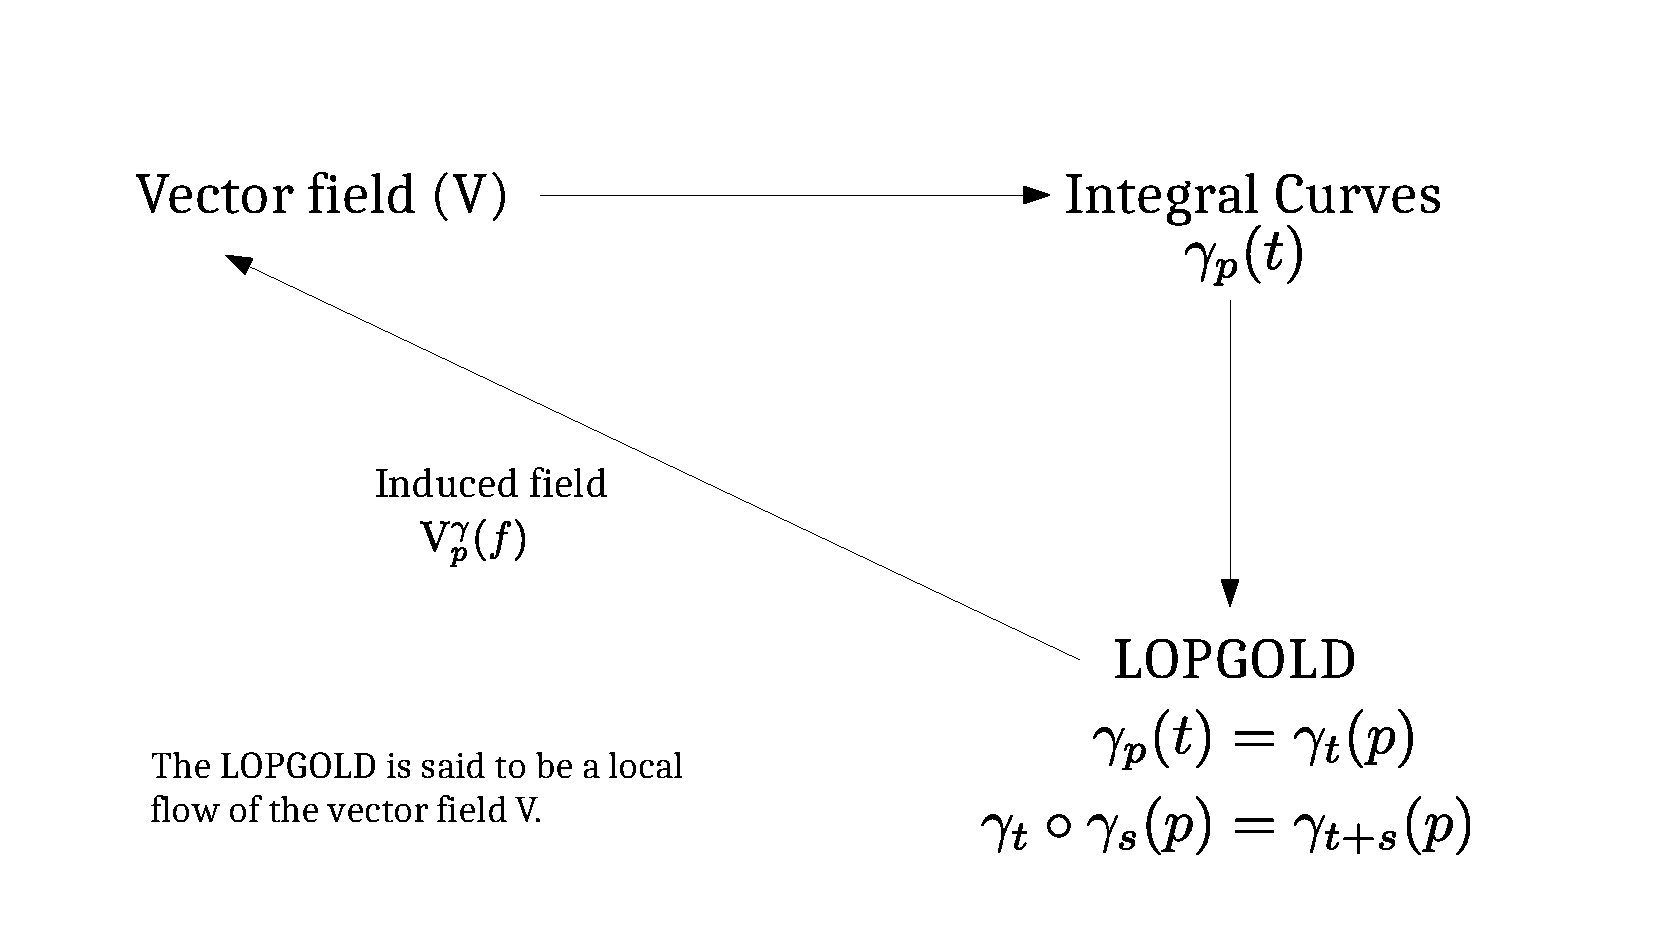
\includegraphics[width=0.8\textwidth, trim={2.3cm 1.2cm 3.1cm
      2.7cm},clip]{vectorFieldLOPGOLDIntegralCurveRelationship}
      \caption[]{}
      \label{fig: relationship between vector field, integral curve and LOPGOLD}
    \end{figure}
  \section{The Lie Derivative}
    Suppose that we have a given vector field $V$, then we know from our
    discussion above that there are local flows associated with this vector
    field. Question: if we are given another vector field $W$, then what is
    the rate of change of $W$ along the flow generated by $V$? To answer this
    question, we need the concept of the Lie derivative of a vector field:
    \begin{definition}[Lie derivative of a vector field]
      Suppose we have two vector fields $V$ and $W$. Then, we define the Lie
      derivative of $W$ with respect to $V$ by:
      \begin{equation}
        \label{eqn: Lie derivative of a vector field}
        \mathcal{L}_{V}W\bigr|_{p} = \lim_{t \rightarrow 0
        }\frac{1}{t}\left[\gamma_{-t*}W_{p'} - W_p\right]
      \end{equation}
      where $\gamma_t$ is a local flow assocaited with $V$ and $p^\prime =
      \gamma_t(p)$.
    \end{definition}
    \begin{remark}
      We can visualise equation~\ref{eqn: Lie derivative of a vector field}
      as shown in Figure~\ref{fig: Lie derivative Definition}. Essentially,
      equation~\ref{eqn: Lie derivative of a vector field} is motivated by
      the fact that we want to compare $W_{p^\prime}$ (the vector field $W$
      at the point $p^\prime$) with $W_p$ (the vector field $W$ at the point
      $p$), where $p^\prime$ is a point along the integral curve of the flow
      $\gamma_p(t)$. However, beacuse we can't compare tangent vectors
      belonging to different tangent spaces, we have to push forward
      $W_{p^\prime}$ to $T_p(\mathcal{M})$, and that is done using the push
      forward map ${\gamma_{-t}}_*$. The Lie derivative is thus the limit
      where $t \to 0$.
      \begin{figure}
        \centering
        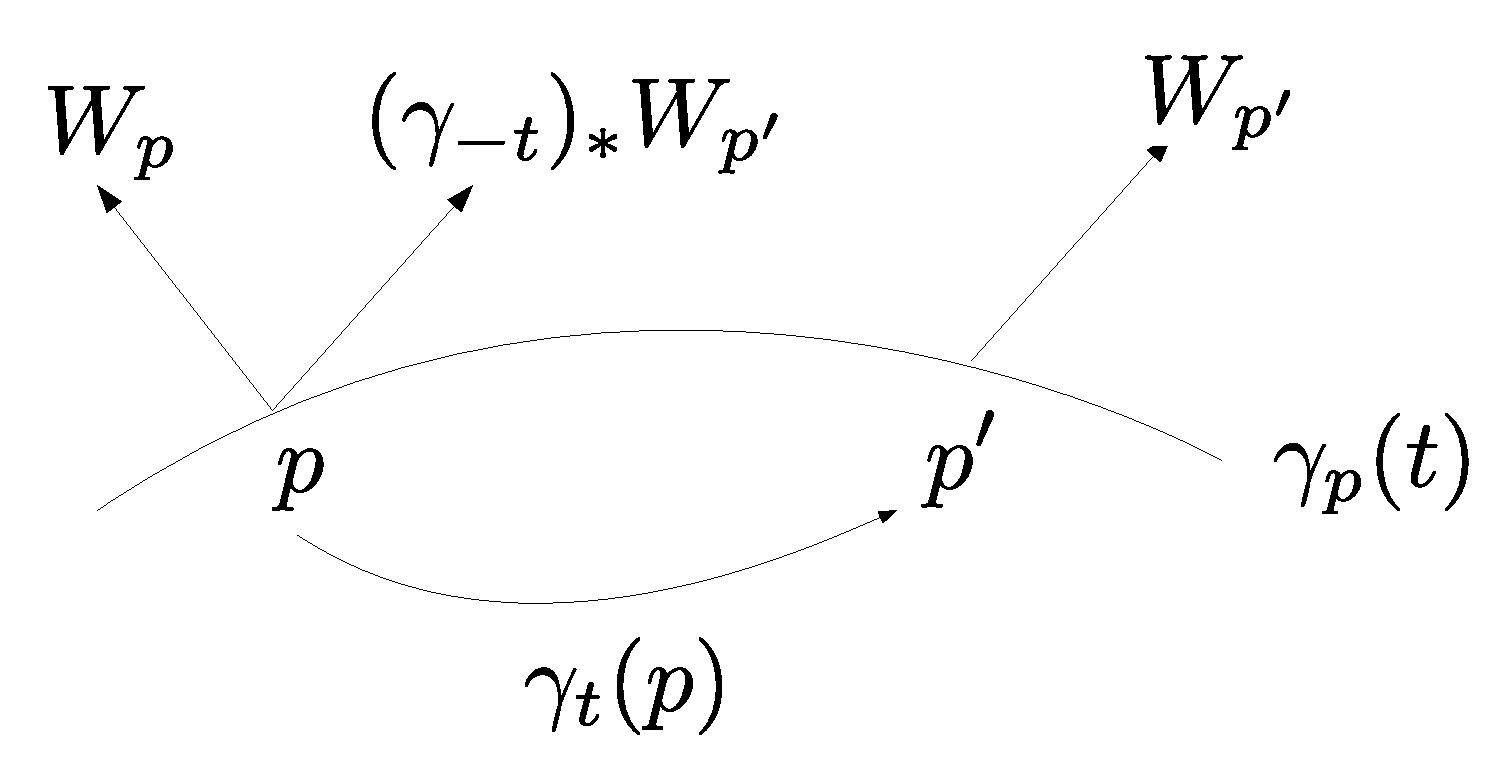
\includegraphics[width=0.6\textwidth, trim={0cm 0cm 0cm
        0cm},clip]{LieDerivativeDefn}
        \caption[]{}
        \label{fig: Lie derivative Definition}
      \end{figure}
    \end{remark}
    We can similarly define the Lie derivative of a one-form, but with the
    pull-back map rather than the push-forward map.
    \begin{definition}[Lie derivative of a one-form]
      \begin{equation}
      \label{eqn: Lie derivative of a one-form}
        \mathcal{L}_{V}\theta\bigr|_{p} = \lim_{t \rightarrow 0
        }\frac{1}{t}\left[\gamma_t^{*} \theta _{p'} - \theta_p\right]
      \end{equation}
    \end{definition}
    \begin{remark}
      Here, we have pulled-back the one-form at $p^\prime$, to the point $p$
      and subtracted $\theta_p$ from it.
    \end{remark}
    The notion of a Lie derivative can be extended to any tensor field in a
    natural way. For instance, if $\mathcal{R} \in T^{(1,1)}$, with
    $\mathcal{R} = W \otimes \theta$, where $W$ is a vector field and
    $\theta$ is a one-form, we define the Lie derivative of $\mathcal{R}$ as:
    \begin{equation}
    \label{eqn: Lie derivative of a 1-1 tensor}
      \mathcal{L}_{V}\mathcal{R}\bigr|_{p} = \lim_{t \rightarrow 0
      }\frac{1}{t}\left[\gamma_{-t*}W_{p'} \otimes \gamma_t^{*}\theta_{p'} -
      W_p \otimes \theta_p \right]
    \end{equation}
    In a similar way, we can extend the notion to any tensor field; just
    pull-back the basis one-forms, and push-forward the basis vectors.

    We note in theorem~\ref{theorem: alternate lie derivative definition}
    that the Lie derivative can be defined in other ways.
    \begin{theorem}[Alternate definitions of the Lie derivative]
      \label{theorem: alternate lie derivative definition}
      Other than equation~\ref{eqn: Lie derivative of a vector field}, the
      Lie derivative can be defined as:
      \begin{align}
        \mathcal{L}_V W\Bigr|_p 
        &= \lim_{t \to 0}[W_p - {\gamma_{t}}_*W_{\gamma_{-t}(p)}] \label{eqn:
        Lie derivative alternate defn 1}\\
        &= \lim_{t \to 0}[W_{\gamma_t(p)} - {\gamma_{t}}_*W_{p}] \label{eqn:
        Lie derivative alternate defn 2}
      \end{align}
    \end{theorem}
    \begin{remark}
      To understand equations~\ref{eqn: Lie derivative alternate defn
      1},\ref{eqn: Lie derivative alternate defn 2}, it is helpful to draw
      figures analogous to Figure~\ref{fig: Lie derivative Definition}.
      \textcolor{red}{Note to self:} These figures will be included in a
      later edition of the notes if I'm free to draw the figures...
    \end{remark}
    \subsection{Properties of Lie derivatives (part 1)}
      Here we use the definition of the Lie derivative to prove some
      properties of the Lie derivative.
        \begin{enumerate}
          \item{Given two tensor fields $R$, $S$ of the same type then:
          \begin{equation}
            \label{eqn: Lie derivative linearity}
            \mathcal{L}_V(R+S) = \mathcal{L}_V(R) + \mathcal{L}_V(S)
          \end{equation}
          \begin{proof}
            This can be shown easily through the linearity of both the
            push-forward and pull-back maps. Using $\gamma_{\pm t*}$ to denote
            both push-forward and pull-back operators respectively, we have:
            \begin{align*}
              \mathcal{L}_V(R+S)\Bigr|_p 
              &= \lim_{t\to 0}\frac{1}{t}\left[\gamma_{\pm
              t*}(R+S)_{p^\prime} - (R+S)_p\right] \\
              &= \lim_{t\to 0}\frac{1}{t}\left[\gamma_{\pm
              t*}R_{p^\prime}+\gamma_{\pm
              t*}S_{p^\prime} - R_p+S_p\right] \\
              &= \lim_{t\to 0}\frac{1}{t}\left[\gamma_{\pm t*}R_{p^\prime}-
              R_p \right]
              +\lim_{t\to 0}\frac{1}{t}\left[\gamma_{\pm
              t*}S_{p^\prime} - S_p\right] \\
              &= \mathcal{L}_V(R) + \mathcal{L}_V(S)
            \end{align*}
          \end{proof}}
          \item{For any two tensor fields $X$ and $Y$, we have:
          \begin{equation}
            \label{eqn: Lie derivative Leibniz rule}
            \mathcal{L}_V(X \otimes Y) = \mathcal{L}_V(X) \otimes Y + X
            \otimes \mathcal{L}_V(Y)
          \end{equation}
          \begin{proof}
            The proof proceeds as follows:
              \[\mathcal{L}_V(X \otimes Y) = \lim_{t \to
              0}\frac{1}{t}\left[\gamma_{\pm t*}X_{p^\prime} \otimes
              \gamma_{\pm t*}Y_{p^\prime} - X_p \otimes Y_p\right]\]
            Subtracting and adding $X_p \otimes \gamma_{\pm t*}Y_{p^\prime}$,
            we have:
            \begin{align*}
              \mathcal{L}_V(X \otimes Y)_p &=\lim_{t \to
              0}\frac{1}{t}\left[\gamma_{\pm t*}X_{p^\prime} \otimes
              \gamma_{\pm t*}Y_{p^\prime} - X_p \otimes \gamma_{\pm
              t*}Y_{p^\prime} + X_p \otimes \gamma_{\pm t*}Y_{p^\prime}- X_p
              \otimes Y_p\right] \\
              &= \lim_{t \to 0}\frac{1}{t}\left[\left(\gamma_{\pm
              t*}X_{p^\prime}- X_p \right) \otimes \gamma_{\pm
              t*}Y_{p^\prime} \right] + \lim_{t \to 0}\frac{1}{t}\left[X_p
              \otimes \left(\gamma_{\pm t*}Y_{p^\prime}-Y_p\right)\right] \\
              &= \mathcal{L}_V(X) \otimes Y\Bigr|_p + X \otimes
              \mathcal{L}_V(Y)\Bigr|_p
            \end{align*}
            which gives the desired result.
          \end{proof}}
        \end{enumerate}
    \subsection{Explicit evaluation of Lie derivatives}
      \subsubsection{Lie derivative of a 0-form (or a function)}
        First, we recall that for a general differentiable map
        $\mathcal{F}:\mathcal{M} \rightarrow \mathcal{N}$ where $\mathcal{M}$
        and $\mathcal{N}$ are two smooth manifolds, the pull-back of
        $f^\prime \in C^\infty(\mathcal{N})$ is: 
        \begin{equation}
          \label{eqn: pull-back of function}
          \mathcal{F}^{*}f^\prime =
          f^\prime \circ \mathcal{F}
        \end{equation}
         The reason for this is that we want
        $\left[\mathcal{F}^{*}f^\prime\right](p) = f^\prime(p^\prime)$, where
        $p^\prime =
        \mathcal{F}(p)$. The situation is shown in Figure~\ref{fig:
        pullBackOfFunction}.
        \begin{figure}
          \centering
          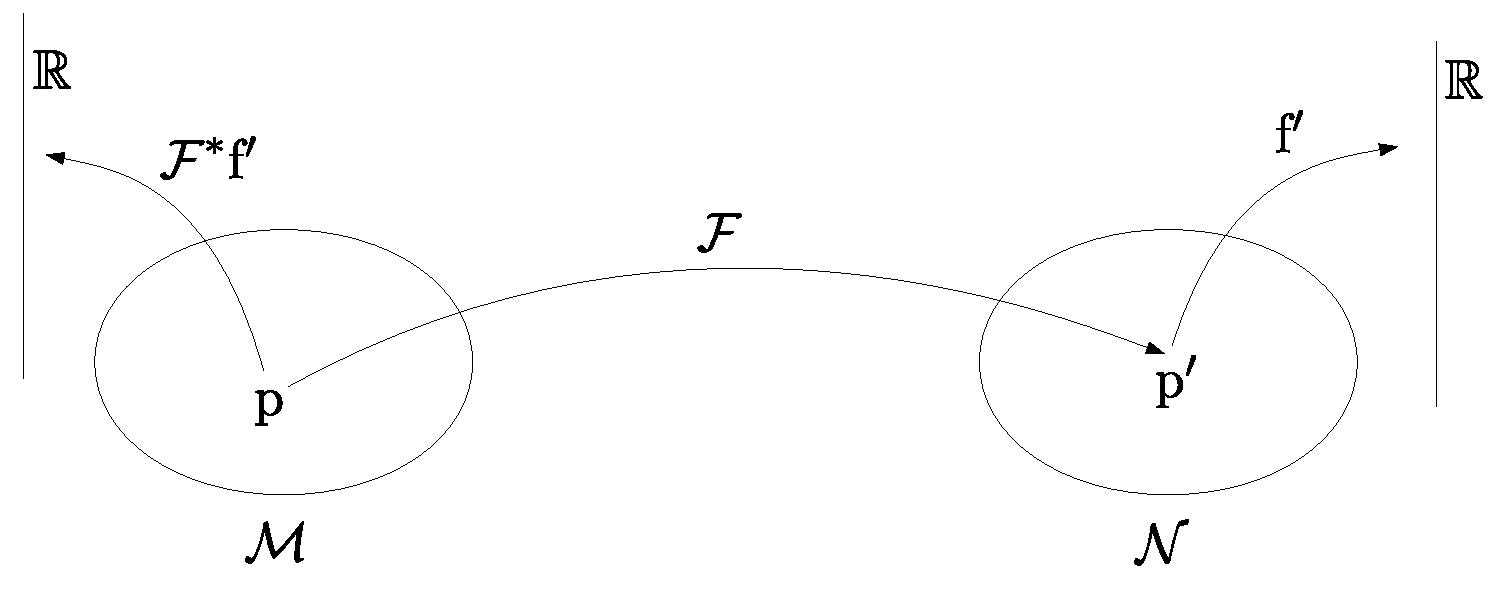
\includegraphics[width=0.75\textwidth, trim={0cm 0cm 0cm
          0cm},clip]{pullBackOfFunction}
          \caption[]{}
          \label{fig: pullBackOfFunction}
        \end{figure}
        Now, we will apply equation~\ref{eqn: pull-back of function} to the
        cases where $\mathcal{F} = \gamma_t(p)$, i.e to the case of a local
        flow. We have:
        \begin{align*}
          \mathcal{L}_V f\Bigr|_p &= \lim_{t\to 0}\frac{1}{t} \left[\gamma^*_t
          f_{p^\prime} - f_p\right] \\
          &= \lim_{t\to 0}\frac{1}{t} \left[f \circ \gamma_t(p) -
          f(p)\right] \\
          &= \lim_{t\to 0}\frac{1}{t} \left[f(\gamma_t(p)) -
          f(p)\right] \\ 
          &= \lim_{t\to 0}\frac{1}{t} \left[f(\gamma_t(p)) -
          f(\gamma_0(p))\right] \\ 
          &=\frac{d}{dt}\left[f \circ \gamma_t(p)\right]\Bigr|_{t=0} \\
          &=\frac{d}{dt}\left[f \circ \gamma_p(t)\right]\Bigr|_{t=0} \\
          &=V^\gamma_p(f) \\
          &=V_p(f)
        \end{align*}
        where to go from the second last line to the last line, we realise
        that $\gamma$ is the integral curve of $V$.

        Thus, we see that the Lie derivative of a function (or a 0-form) is
        just the directional derivative of that function.
      \subsubsection{Lie derivative of a vector field $W$}
        Now, we go back to our original scenario in equation~\ref{eqn: Lie
        derivative of a vector field}, reproduced here for convenience:
        \[\mathcal{L}_{V}W\bigr|_{p} = \lim_{t \rightarrow 0
        }\frac{1}{t}\left[\gamma_{-t*}W_{p'} - W_p\right]\]
        We shall evaluate equation~\ref{eqn: Lie derivative of a vector
        field} in a local chart $(U,\phi)$ with coordinates $\phi(p) =
        (x^1,...,x^m)$. Our strategy will be first consider $W =
        \frac{\partial}{\partial x^i}$, i.e we consider a basis field first.
        Then, we can find the expression for a general vector field.

        In the local chart $(U,\phi)$, we shall make the following
        identifications:
        \begin{gather*}
          \phi(p) = x \equiv (x^1,...,x^m)\\
          \phi(p^\prime) = y \equiv (y^1,...,y^m)\\
          \gamma_t(p) = p^\prime \xRightarrow[(U,\phi)]{\text{Local chart}}
          \overline{\gamma}_t(x) = y \\
          W_{p^\prime} \xrightarrow[(U,\phi)]{\text{Local chart}}
          \overline{W}_y \quad \quad
          W_{p} \xrightarrow[(U,\phi)]{\text{Local chart}}
          \overline{W}_x
        \end{gather*}
        Note also that since $p$ and $p^\prime$ lie on the same integral
        curve $\gamma_p(t)$, we have:
        \begin{gather*}
          \gamma_p(t) = p^\prime \xRightarrow[(U,\phi)]{\text{Local chart}}
          \overline{\gamma}_x(t) = (x^1(t),...,x^m(t)) = (y^1,...,y^m) \\
          \gamma_p(0) = p^\prime \xRightarrow[(U,\phi)]{\text{Local chart}}
          \overline{\gamma}_x(0) = (x^1(0),...,x^m(0)) = (x^1,...,x^m)
        \end{gather*}
        where the second line above is a direct consequence of the first. All
        of this is shown nicely in Figure~\ref{fig: Lie derivative of vector
        field evaluation}.
        \begin{figure}
          \centering
          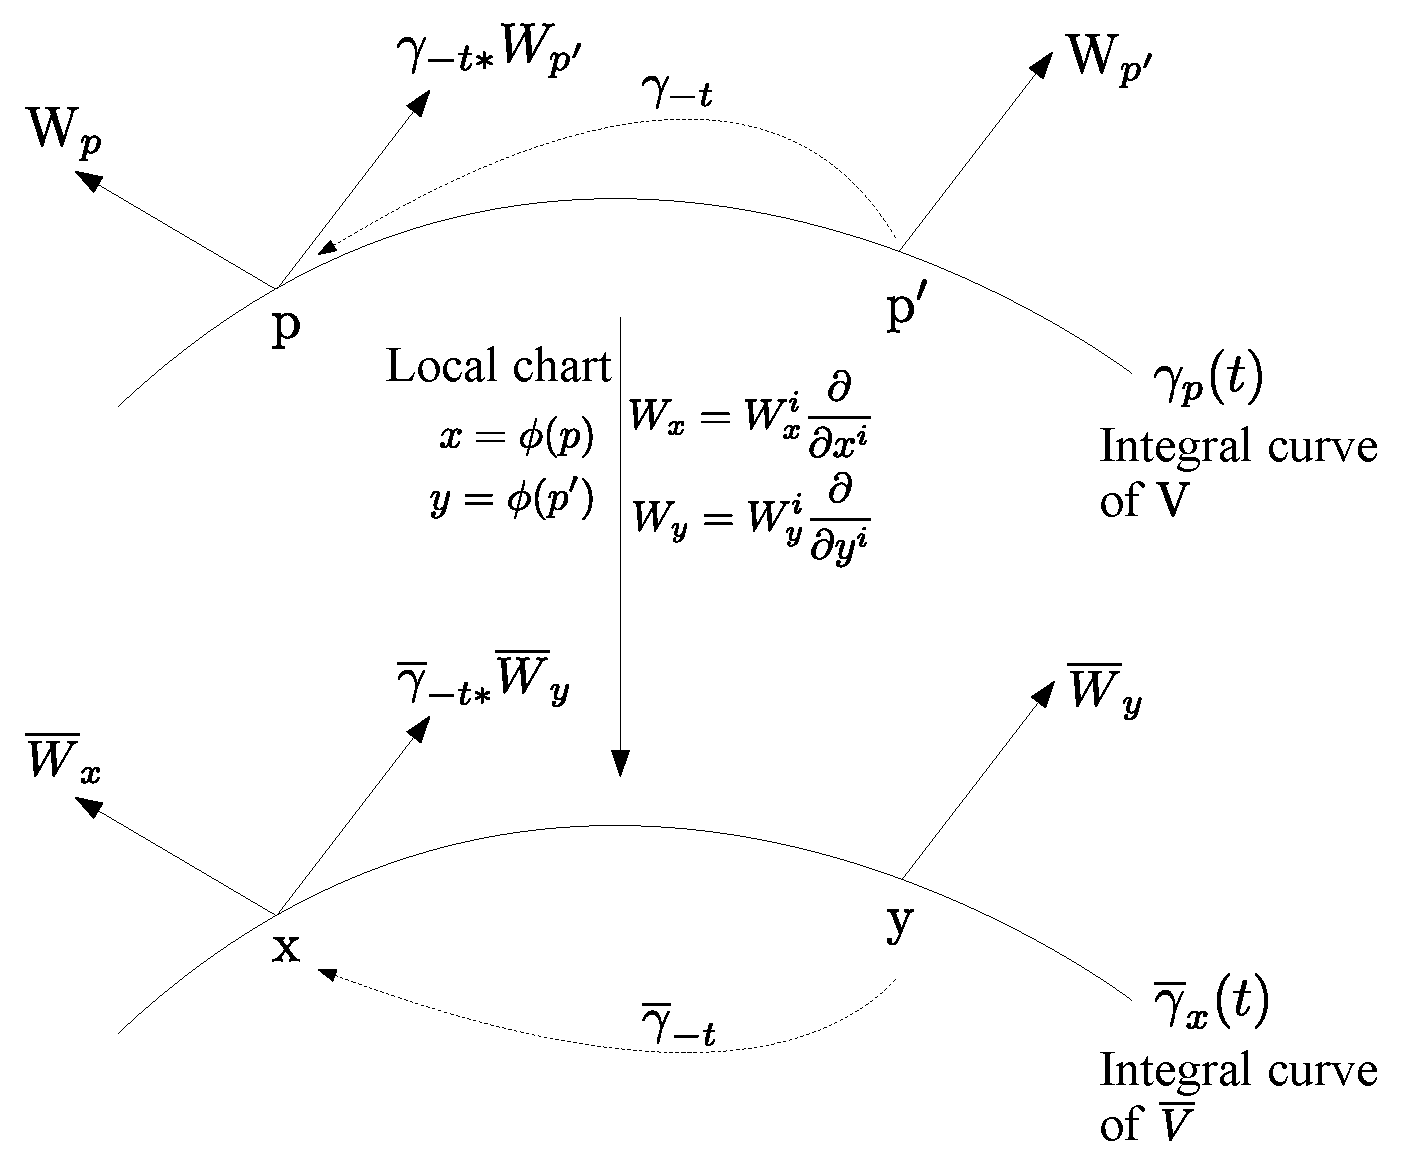
\includegraphics[width=0.8\textwidth, trim={0cm 0cm 0cm
          0cm},clip]{LieDerivativeOfVectorFieldEvaluation}
          \caption[]{}
          \label{fig: Lie derivative of vector field evaluation}
        \end{figure}
        Thus, in a local chart $(U,\phi)$, the Lie derivative definition
        looks like:
        \begin{equation}
          \label{eqn: Lie derivative vector field evaluation local chart}
          \mathcal{L}_{\overline{V}}\overline{W}\Bigr|_x = \lim_{t \to
          0}\frac{1}{t}\left[\overline{\gamma}_{-t*}\overline{W}_y -
          \overline{W}_x \right]
        \end{equation}
        Let's explicitly evaluate equation~\ref{eqn: Lie derivative vector
        field evaluation local chart} by first evaluating
        $\overline{\gamma}_{-t*}\overline{W}_y\left(\bar{f}\right)$, where
        $\bar{f} \in C^\infty(\mathbb{R})$ is a function of $x$. Now,
        \begin{align*}
          \overline{\gamma}_{-t*}\overline{W}_y\left(\bar{f}\right) 
          &= \overline{W}_y\left(\bar{f}\circ \gamma_{-t}(y)\right)
        \end{align*}
        Using the fact that according to Figure~\ref{fig: Lie derivative of
        vector field evaluation}, $\gamma_{-t}(y)$ gives us $m$ equations of
        the form $x^i = x^i(y^1,...,y^m)$, where $i = 1,..,m$, we have:
        \begin{align*}
          \overline{\gamma}_{-t*}\overline{W}_y\left(\bar{f}\right) 
          &=
          \overline{W}_y\left(\bar{f}(x^1(y^1,...,y^m),...,x^m(y^1,...,y^m))\right)
          \\
          &=
          \overline{W}^k_y\frac{\partial}{\partial
          y^k}\left(\bar{f}(x^1(y^1,...,y^m),...,x^m(y^1,...,y^m))\right) \\
          &=\overline{W}^k_y\frac{\partial \bar{f}}{\partial
          x^j}\frac{\partial x^j}{\partial y^k}\\
          &= \overline{W}^k_y\frac{\partial \bar{f}}{\partial
          x^j}\frac{\partial \overline{\gamma}_{-t}^j}{\partial y^k} \\
          &= \overline{W}^k_y\frac{\partial
          \overline{\gamma}_{-t}^j}{\partial y^k}\frac{\partial
          \bar{f}}{\partial x^j}
        \end{align*}
        Substituting the above result into equation~\ref{eqn: Lie
        derivative vector field evaluation local chart}, we have:
        \begin{align*}
          \mathcal{L}_{\overline{V}}\overline{W}\Bigr|_x \bar{f}
          &= \lim_{t \to
          0}\frac{1}{t}\left[\overline{\gamma}_{-t*}\overline{W}_y -
          \overline{W}_x \right]\left(\bar{f}\right) \\
          &= \lim_{t \to
          0}\frac{1}{t}\left[ \overline{W}^k_y\frac{\partial
          \overline{\gamma}_{-t}^j}{\partial y^k}\frac{\partial
          \bar{f}}{\partial x^j} -
          \overline{W}^k_x\frac{\partial \bar{f}}{\partial x^k} \right]
        \end{align*}
        Now, we restrict ourselves to the basis field $\overline{W} =
        \dfrac{\partial}{\partial x^i}$, which gives us:
        \[\overline{W}_x^k =\overline{W}_x^k = \delta^k_i \]
        Then, we have:
        \begin{align*}
          \mathcal{L}_{\overline{V}}\left(\frac{\partial}{\partial
          x^i}\right)\Bigr|_x \bar{f}
          &= \lim_{t \to 0}\frac{1}{t}\left[ \delta^k_i \frac{\partial
          \overline{\gamma}_{-t}^j}{\partial y^k}\frac{\partial
          \bar{f}}{\partial x^j} - \delta^k_i\frac{\partial \bar{f}}{\partial
          x^k} \right] \\
          &= \lim_{t \to 0}\frac{1}{t}\left[\frac{\partial
          \overline{\gamma}_{-t}^j}{\partial y^i}\frac{\partial
          \bar{f}}{\partial x^j} - \delta^k_i\frac{\partial \bar{f}}{\partial
          x^k} \right]
        \end{align*}
        Using some mathematical trickery, i.e $\delta_i^k = \dfrac{\partial
        y^k}{\partial y^i}$, we have:
        \begin{align*}
          \mathcal{L}_{\overline{V}}\left(\frac{\partial}{\partial
          x^i}\right)\Bigr|_x \bar{f}
          &= \lim_{t \to 0}\frac{1}{t}\left[\frac{\partial
          \overline{\gamma}_{-t}^j}{\partial y^i}\frac{\partial
          \bar{f}}{\partial x^j} - \frac{\partial y^k}{\partial
          y^i}\frac{\partial \bar{f}}{\partial x^k} \right]\\
          &= \lim_{t \to 0}\frac{1}{t}\left[\frac{\partial
          \overline{\gamma}_{-t}^j}{\partial y^i}\frac{\partial
          \bar{f}}{\partial x^j} - \frac{\partial
          \overline{\gamma}^j_{0}}{\partial y^i}\frac{\partial
          \bar{f}}{\partial x^j} \right] \\
        \end{align*}
        where we note that $\gamma_0$ is the identity map, i.e $\gamma_0(y) =
        y$. Making the $y$ dependence of $\gamma_{-t}^j$ explicit, we
        have\footnote{The derivation from here onwards departs from Kuldip's
        treatment, not sure how legit it is. The departure is because
        Kuldip's treatment seems sketchy...}:
        \begin{align*}
          \mathcal{L}_{\overline{V}}\left(\frac{\partial}{\partial
          x^i}\right)\Bigr|_x \bar{f}
          &= \lim_{t \to 0}\frac{1}{t}\left[\frac{\partial
          \overline{\gamma}_{-t}^j(y^1,...,y^m)}{\partial
          y^i}\frac{\partial \bar{f}}{\partial x^j} -
          \frac{\partial
          \overline{\gamma}^j_{0}(y^1,...,y^m)}{\partial
          y^i}\frac{\partial \bar{f}}{\partial x^j} \right] \\
          &= \lim_{t \to 0}\frac{1}{t}\left[\frac{\partial
          \overline{\gamma}_{-t}^j(y^1,...,y^m)}{\partial y^i} -
          \frac{\partial \overline{\gamma}^j_{0}(y^1,...,y^m)}{\partial y^i}
          \right]\frac{\partial \bar{f}}{\partial x^j}
        \end{align*}
        Now, making the substitution $s = -t$, we have:
        \begin{align*}
          \mathcal{L}_{\overline{V}}\left(\frac{\partial}{\partial
          x^i}\right)\Bigr|_x \bar{f}
          &= -\lim_{s \to 0}\frac{1}{s}\left[\frac{\partial
          \overline{\gamma}_{s}^j(y^1,...,y^m)}{\partial y^i} -
          \frac{\partial \overline{\gamma}^j_{0}(y^1,...,y^m)}{\partial
          y^i}\right] \frac{\partial \bar{f}}{\partial x^j} \\
          &= -\lim_{s \to 0}\left[\frac{\partial}{\partial
          y^i}\left(\frac{\overline{\gamma}_{s}^j(y^1,...,y^m) -
          \overline{\gamma}_{0}^j(y^1,...,y^m)}{s}\right)
          \right]\frac{\partial \bar{f}}{\partial x^j}
        \end{align*}
        Now, the limit in the last line above is a tricky limit to take. We
        first realise that $s \to 0 \implies t \to 0$, and $t \to 0 \implies
        y \to x$. Thus, this allows us to do:
        \begin{align*}
          \mathcal{L}_{\overline{V}}\left(\frac{\partial}{\partial
          x^i}\right)\Bigr|_x \bar{f}
          &= -\lim_{s \to 0}\left[\frac{\partial}{\partial
          x^i}\left(\frac{\overline{\gamma}_{s}^j(x^1,...,x^m) -
          \overline{\gamma}_{0}^j(x^1,...,x^m)}{s}\right)
          \right]\frac{\partial \bar{f}}{\partial x^j}
        \end{align*}
        which then gives us:
        \begin{align*}
          \mathcal{L}_{\overline{V}}\left(\frac{\partial}{\partial
          x^i}\right)\Bigr|_x \bar{f} 
          &= -\frac{\partial}{\partial x^i}\left(\frac{d
          \overline{\gamma}_s^j(x^1,...,x^m)}{ds}\Bigr|_{s=0}\right)
          \frac{\partial \bar{f}}{\partial x^j} \\
          &= -\frac{\partial}{\partial x^i}\left(\frac{d
          \overline{\gamma}_x^j(s)}{ds}\Bigr|_{s=0}\right)
          \frac{\partial \bar{f}}{\partial x^j}
        \end{align*}
        Realising that $\dfrac{d \overline{\gamma}_x^j(s)}{ds}$ is $j$-th
        component of the tangent vector to the integral curve at the point
        $x$, which is just another way to refer to the $j$-th component of
        the vector field $\overline{V}_x$, we have:
        \begin{equation}
          \label{eqn: Lie derivative of basis field}
          \mathcal{L}_{\overline{V}}\left(\frac{\partial}{\partial
          x^i}\right)\Bigr|_x = -\frac{\partial}{\partial
          x^i}\left(\overline{V}^j_x\right) \frac{\partial \bar{f}}{\partial
          x^j}
        \end{equation}
        Now that we have equation~\ref{eqn: Lie derivative of basis field},
        we can easily extend our results to include any field $\overline{W} =
        \overline{W}^i\dfrac{\partial}{\partial x^i}$ using
        equation~\ref{eqn: Lie derivative linearity} and equation~\ref{eqn:
        Lie derivative Leibniz rule}. I.e, we can write:
        \begin{align*}
          \overline{W} &= \overline{W}^i\dfrac{\partial}{\partial x^i} \\ 
          &= \overline{W}^1\frac{\partial}{\partial x^1} +
          \overline{W}^2\frac{\partial}{\partial x^2} + ... +
          \overline{W}^m\dfrac{\partial}{\partial x^m}
        \end{align*}
        which gives us
        \begin{align*}
          \mathcal{L}_{\overline{V}}\overline{W}
          &=
          \mathcal{L}_{\overline{V}}\left(\overline{W}^i\frac{\partial}{\partial
          x^i}\right) \\
          &=
          \mathcal{L}_{\overline{V}}\left(\overline{W}^1\frac{\partial}{\partial
          x^1}\right) +
          \mathcal{L}_{\overline{V}}\left(\overline{W}^2\frac{\partial}{\partial
          x^2}\right) + ... +
          \mathcal{L}_{\overline{V}}\left(\overline{W}^m\dfrac{\partial}{\partial
          x^m}\right)
        \end{align*}
        and note that for each individual term in the summation, say
        $\mathcal{L}_{\overline{V}}\left(\overline{W}^1\dfrac{\partial}{\partial
        x^1}\right)$, we can treat $\overline{W}^1$ as a 0-form and
        $\dfrac{\partial}{\partial x^1}$ as a vector and then apply
        equation~\ref{eqn: Lie derivative Leibniz rule}. E.g:
        \begin{align*}
          \mathcal{L}_{\overline{V}}\left(\overline{W}^1\frac{\partial}{\partial
          x^1}\right)
          &=
          \mathcal{L}_{\overline{V}}\left(\overline{W}^1\right) +
          \frac{\partial}{\partial
          x^1}
          \overline{W}^1\mathcal{L}_{\overline{V}}\left(\frac{\partial}{\partial
          x^1}\right) \\
          &= V^j \frac{\partial \overline{W}^1}{\partial
          x^j}\frac{\partial}{\partial x^1} + \overline{W}^1
          \left(-\frac{\partial}{\partial x^1}\left(\overline{V}^j\right)
          \frac{\partial}{\partial x^j}\right) \\
          &= V^j\frac{\partial \overline{W}^1}{\partial
          x^j}\frac{\partial}{\partial x^1} - \overline{W}^1 \frac{\partial
          \overline{V}^j}{\partial x^1}\frac{\partial}{\partial x^j}
        \end{align*}
        Thus, summing over all these individual terms, we have:
        \begin{align*}
          \mathcal{L}_{\overline{V}}\left(\overline{W}^i\frac{\partial}{\partial
          x^i}\right) &=
          V^j\frac{\partial \overline{W}^i}{\partial
          x^j}\frac{\partial}{\partial x^i} - \overline{W}^i \frac{\partial
          \overline{V}^j}{\partial x^i}\frac{\partial}{\partial x^j}
        \end{align*}
        Doing a renaming of dummy variables for the first term, i.e the good
        old $ i\leftrightarrow j$, we have:
        \begin{align*}
          \mathcal{L}_{\overline{V}}\left(\overline{W}^i\frac{\partial}{\partial
          x^i}\right) 
          &= V^i\frac{\partial \overline{W}^j}{\partial
          x^i}\frac{\partial}{\partial x^j} - \overline{W}^i \frac{\partial
          \overline{V}^j}{\partial x^i}\frac{\partial}{\partial x^j} \\
          &=\left(V^i\frac{\partial \overline{W}^j}{\partial x^i} -
          \overline{W}^i \frac{\partial \overline{V}^j}{\partial x^i}
          \right)\frac{\partial}{\partial x^j}
        \end{align*}
        With reference to equation~\ref{eqn: commutator in local chart},
        notice that the last line is exactly how the the commutator of
        $\overline{V}$ and $\overline{W}$ looks like. This gives us our very
        interesting result:
        \begin{equation}
          \mathcal{L}_{\overline{V}}\overline{W} =
          \left[\overline{V},\overline{W}\right]
        \end{equation}
        and this is the reason why the commutator is also called the Lie
        bracket.
      \subsubsection{Lie derivative of a one-form}
        Here, we want to evaluate equation~\ref{eqn: Lie derivative of a
        one-form} in a local chart $(U,\phi)$, which we will write as:
        \begin{equation}
          \label{eqn: Lie derivative one-form local chart}
          \mathcal{L}_{\overline{V}} \overline{\theta} = \lim_{t\to
          0}\frac{1}{t}\left[\overline{\gamma}_t^* \overline{\theta}_y -
          \overline{\theta}_x\right]
        \end{equation}
        To get from equation~\ref{eqn: Lie derivative of a one-form} to
        equation~\ref{eqn: Lie derivative one-form local chart}, we have made
        the folllowing substitutions:
        \begin{align*}
          \phi(p) = x, &\quad \quad \quad \quad \phi(p^\prime) = y \\
          p^\prime = \gamma_t(p) &\xRightarrow[(U,\phi)]{\text{Local Chart}}
          y = \gamma_t(x)\\
          \theta_{p^\prime} &\xrightarrow[(U,\phi)]{\text{Local Chart}}
          \overline{\theta}_y \\
          \theta_{p} &\xrightarrow[(U,\phi)]{\text{Local Chart}}
          \overline{\theta}_x
        \end{align*}
        Note that the second equation above gives us $m$ coordinate
        transformation equations of the form: $y^i = y^i(x^1,...,x^m)$ for $i
        = 1,2,...,m$. Now, we first evaluate the $\overline{\gamma}_t^*
        \overline{\theta}_y$ term. We first have:
        \begin{align*}
          \left\langle \overline{\gamma}_t^* \overline{\theta}_y, \,
          \frac{\partial}{\partial x^i} \right\rangle
          &= \left\langle  \overline{\theta}_y, \,
          {\overline{\gamma}_t}_*\frac{\partial}{\partial x^i} \right\rangle
        \end{align*}
        Next, we note that, for $\bar{f}^\prime \in C^\infty(\mathcal{M})$
        where $\bar{f}^\prime$ is a function of $y$, we have, using
        theorem~\ref{theorem: f-related field calculation},
        \begin{align*}
          \left[{\overline{\gamma}_t}_*\frac{\partial}{\partial x^i}
          \bar{f}^\prime\right](y) 
          &= \frac{\partial}{\partial x^i}\left(\bar{f}^\prime \circ
          \overline{\gamma}_t(x^1,...,x^m) \right) \\
          &= \frac{\partial \bar{f}^\prime\left(
          \overline{\gamma}_t(x^1,...,x^m) \right)}{\partial x^i} \\
          &= \frac{\partial \bar{f}^\prime\left(
          y^1(x^1,...,x^m),...,y^m(x^1,...,x^m) \right)}{\partial x^i}\\
          &= \frac{\partial \bar{f}^\prime}{\partial y^j}\frac{\partial
          y^j}{\partial x^i}
        \end{align*}
        Noting that $\dfrac{\partial y^j}{\partial x^i} = \dfrac{\partial
        \overline{\gamma}_t^j(x^1,...,x^m)}{\partial x^i}$, our result above
        becomes:
        \[\left[{\overline{\gamma}_t}_*\frac{\partial}{\partial x^i}
        \bar{f}^\prime\right](y) = \frac{\partial
        \overline{\gamma}_t^j(x^1,...,x^m)}{\partial x^i}\frac{\partial
        \bar{f}^\prime}{\partial y^j}\]
        which gives us:
        \[{\overline{\gamma}_t}_*\frac{\partial}{\partial x^i} =
        \frac{\partial \overline{\gamma}_t^j(x^1,...,x^m)}{\partial
        x^i}\frac{\partial }{\partial y^j}\]
        Continuing with our evaluation of $\overline{\gamma}_t^*
        \overline{\theta}_y$, we have:
        \begin{align*}
          \left\langle \overline{\gamma}_t^* \overline{\theta}_y, \,
          \frac{\partial}{\partial x^i} \right\rangle
          &= \left\langle  \overline{\theta}_y, \,
          {\overline{\gamma}_t}_*\frac{\partial}{\partial x^i} \right\rangle \\
          &=\left\langle\overline{\theta}_y, \,\frac{\partial
          \overline{\gamma}_t^j(x^1,...,x^m)}{\partial x^i}\frac{\partial
          }{\partial y^j} \right\rangle \\
          &= \frac{\partial \overline{\gamma}_t^j(x^1,...,x^m)}{\partial
          x^i}\left\langle\overline{\theta}_y, \,\frac{\partial }{\partial
          y^j} \right\rangle \\
          &= \frac{\partial \overline{\gamma}_t^j(x^1,...,x^m)}{\partial
          x^i} \left(\overline{\theta}_y\right)_j \\
          &=\frac{\partial \overline{\gamma}_x^j(t)}{\partial
          x^i} \left(\overline{\theta}_y\right)_j
        \end{align*}
        where in the last line, we note that for a local flow
        $\overline{\gamma}_t$, we have $\overline{\gamma}_t(x) =
        \overline{\gamma}_x(t)$. Thus, this gives us: \[\overline{\gamma}_t^*
        \overline{\theta}_y = \frac{\partial
        \overline{\gamma}_x^j(t)}{\partial x^i}
        \left(\overline{\theta}_y\right)_j dx^i \]
        Substituting the above result into equation~\ref{eqn: Lie derivative
        one-form local chart}, we have:
        \begin{align*}
          \mathcal{L}_{\overline{V}} \overline{\theta} &= \lim_{t\to
          0}\frac{1}{t}\left[\overline{\gamma}_t^* \overline{\theta}_y -
          \overline{\theta}_x\right] \\ &=\lim_{t\to
          0}\frac{1}{t}\left[\frac{\partial
          \overline{\gamma}_x^j(t)}{\partial x^i}
          \left(\overline{\theta}_y\right)_j dx^i -
          \left(\overline{\theta}_x\right)_i dx^i\right]
        \end{align*}
        Now, we first consider a basis one-form, i.e we consider
        $\overline{\theta} = \delta_i^k dx^i = dx^k$. Then, we have:
        \begin{align*}
          \mathcal{L}_{\overline{V}} dx^k &=\lim_{t\to
          0}\frac{1}{t}\left[\frac{\partial
          \overline{\gamma}_x^j(t)}{\partial x^i} \delta_j^k dx^i -
          \delta_i^k dx^i\right] \\
          &=\lim_{t\to 0}\frac{1}{t}\left[\frac{\partial
          \overline{\gamma}_x^k(t)}{\partial x^i} dx^i - \frac{\partial
          x^k}{\partial x^i} dx^i\right] \\
          &=\lim_{t\to 0}\frac{1}{t}\left[\frac{\partial
          \overline{\gamma}_x^k(t)}{\partial x^i} dx^i - \frac{\partial
          \overline{\gamma}^k_x(0)}{\partial x^i} dx^i\right] \\
          &=\lim_{t\to 0}\frac{1}{t}\left[\frac{\partial
          \overline{\gamma}_x^k(t)}{\partial x^i} - \frac{\partial
          \overline{\gamma}^k_x(0)}{\partial x^i} \right] dx^i \\
          &=\lim_{t\to 0} \frac{\partial}{\partial
          x^i}\left[\frac{\gamma_x^k(t) - \gamma_x^k(0)}{t}\right] dx^i \\
          &=\frac{\partial}{\partial
          x^i}\left(\frac{d\overline{\gamma}_x^k}{dt}\right)\Biggr|_{t=0}
          dx^i
        \end{align*}
        Noting that $\dfrac{\partial}{\partial
        x^i}\left(\frac{d\overline{\gamma}_x^k}{dt}\right)\Biggr|_{t=0}$ is
        nothing more than the $k$-th component of the tangent vector to the
        integral curve $\gamma_x(t)$, which is the $k$-th component of the
        vector field $\overline{V}$ at $x$, we have:
        \begin{align}
        \mathcal{L}_{\overline{V}} dx^k 
        &=\frac{\partial}{\partial x^i}\left(V^k_x\right) dx^i \nonumber\\
        &=\frac{\partial V^k}{\partial x^i}dx^i
        \end{align}
        The equation above can then be used to evaluate the Lie derivative of
        any arbitrary one-form $\theta_i dx^i$, using both equation~\ref{eqn:
        Lie derivative linearity} and equation~\ref{eqn: Lie derivative
        Leibniz rule}. \textcolor{red}{This is left as an exercise
        to...future KH or whoever reads this notes}\footnote{This exercise is
        rather simple, just follow the same steps as when finding the Lie
        derivative of an arbitary vector field given the Lie derivative of
        the basis vector.}.

        Now, we shall state one very important result in the evaluation of
        Lie derivatives:
        \begin{theorem}
          \label{theorem: Lie derivative of one form theorem}
          In a local chart, for a vector field $\overline{V}$ and a one-form
          $\overline{\omega}$ we have:
          \begin{equation}
            \mathcal{L}_{\overline{V}}\overline{\omega} =
            d\left(\overline{\omega}(\overline{V})\right) +
            (d\overline{\omega})(\overline{V})
          \end{equation}
          where $d$ stands for the exterior derivative operator\footnote{To
          be introduced in a later chapter.}.
        \end{theorem}
        \begin{proof}
          \textcolor{red}{To fill in next time}
        \end{proof}
        \begin{remark}
          According to Kuldip's lecture notes, theorem~\ref{theorem: Lie
          derivative of one form theorem} holds for $2$-forms too. I wonder
          if it holds for $n$ forms; \textcolor{red}{we can try to prove this
          next time.}
        \end{remark}
    \subsection{Properties of the Lie derivative (Part 2)}
      Now that we can explicitly evaluate the Lie derivative for a scalar
      field, vector field and one-form, we can show that for a tensor $T$ in
      general, the following two properties are true:
      \begin{subequations}
        \label{eqn: Two other properties of Lie derivatives (for Lie Algebra)}
        \begin{gather}
          \mathcal{L}_{a V + b W}T = a\mathcal{L}_V T + b\mathcal{L}_W T \\
          \mathcal{L}_{[V,W]}T = \mathcal{L}_V\left(\mathcal{L}_W(T)\right)
          -\mathcal{L}_W\left(\mathcal{L}_V(T) \right)
        \end{gather}
    \end{subequations}
      \begin{proof}[Rough sketch of a proof for now]
        Since an arbitrary tensor is just of the form $T =
        T_{abc...}^{def...} \partial_d \otimes \partial_e \otimes \partial_f
        \otimes dx^a \otimes dx^b \otimes dx^c$, we can first prove these two
        equations individually for a scalar field, vector field and for a
        one-form (\textcolor{red}{To be done in the
        future\footnote{Alternatively, see Edward Teo's PC4274 tutorial
        3}.}), then apply equation~\ref{eqn: Lie derivative linearity} and
        equation~\ref{eqn: Lie derivative Leibniz rule}.
      \end{proof}
      Now, the above two properties naturally lead us to the notion of Lie
      algebras. But first, let us define what an invariant tensor field is
      first.
      \begin{definition}[Invariant tensor field]
        A tensor field $T$ is said to be invariant under a vector field $V$ if
        \[\mathcal{L}_V(T) = 0\]
        We sometimes also say that $T$ is Lie-dragged by $V$.
      \end{definition}
      \begin{remark}
        In other words, this means that as we move along the local flow
        generated by the vector field $V$, the tensor $T$ remains unchanged.
      \end{remark}
      Now, equation~\ref{eqn: Two other properties of Lie derivatives (for
      Lie Algebra)} implies that when $T$ is invariant under $V$ and $W$,
      then it is invariant under $aV+bW$ and $[V,W]$. We say that the set of
      all fields which $T$ is invariant under forms a Lie algebra. This shows
      the intimate relationship beween invariances (or symmetries) and Lie
      algebras. This idea will be explored further in a later chapter on Lie
      algebras.
    \subsection{Lie derivative and the coordinate basis}
      See Edward teo's notes chapter 3 for now, \textcolor{red}{Will add
      later when I have time.}
    % \include{chapterEightnForms}
    % \include{chapterNineExteriorDifferentiation}
    % \include{chapterTenMetricTensor}
    % \include{chapterElevenExteriorCalculus}
    \chapter*{Things yet to be written:}
\begin{enumerate}
  \item{Chapter 1, basic topo}
  \item{Chapter 6, contraction of tensors and how that relates to the tensor
  product}
  \item{Chapter 7, all the red stuff}
  \item{All the exterior algebra stuff}
\end{enumerate}
  
\end{document}